% *******************************************************************
% STOP - Bitte zuerst lesen, bevor Sie weitermachen
%
% Einige Dinge müssen Sie an Ihre Bedürfnisse (und die Vorgaben Ihres
% Betreuers anpassen).
%
% 1. Sprache
% Das Template unterstützt Deutsch und Englisch, Standard ist Deutsch.
% Wenn Sie Englisch verwenden wollen, ändern Sie bitte direkt am Anfang
% dieser Datei den Eintrag
%    \newcommand{\hsmasprache}{de}
% auf
%    \newcommand{\hsmasprache}{en}
%
% 2. Zitierstil
% Abhängig von dem gewünschten Zitierstil passen Sie bitte in
% preambel.tex die Einstellungen bei \usepackage[backend=biber...
% an. Wie ist dort genau erklärt.
%
% 3. Doppelseitiger oder einseitiger Druck
% Das Template ist für doppelseitigen Druck eingestellt. Wollen Sie
% einseitig drucken, müssen Sie in preambel.tex die Einstellungen
% für \documentclass ändern. Und zwar von twoside=on auf twoside=off.
%
% 4. Abkürzungen auf richtige Breite einstellen
% In der Datei kapitel/abkuerzungen.tex müssen Sie die _längste_
% Abkürzung in die eckigen Klammern von \begin{acronym} schreiben,
% sonst werden die Abkürzungen nicht richtig ausgerichtet.
% Also z.B. \begin{acronym}[DSGVO].
%
% 5. Unnötige Teile entfernen
% Entfernen Sie die Teile, die Sie nicht brauchen, z.B. Anhänge,
% Quelltextverzeichnis etc. Siehe unten
%
% 6. Silbentrennung
% LaTeX führt eine automatische Silbentrennung durch. Allerdings
% werden Wörter, die bereits einen Bindestrich enthalten nicht
% getrennt, z.B. Datenschutz-Grundverordnung. Wenn Sie Ihren Text auf
% Deutsch schreiben, können Sie dann alternativ "= für den Bindestrich
% im Wort verwenden, z.B. Datenschutz"=Grundverordnung, damit LaTeX
% weiterhin richtig trennt.
% Ist die Silbentrennung aus einem anderen Grund nicht erfolgt, sodass
% das Wort über den rechten Rand hinaussteht oder wenn Sie eine weitere
% Trennstelle wollen, können Sie LaTeX helfen, indem Sie weitere
% Trennstellen angeben. Dies geschieht durch "- als Zeichen, z.B.
% Staats"-vertrag.
%
% 7. Nummerierung der Fußnoten
% LaTeX beginnt die Nummerierung der Fußnoten in jedem Kapitel wieder
% bei 1. Manche Dozenten wollen aber eine durchlaufende Nummerierung
% über die gesamte Arbeit. In diesem Fall gehen Sie in die preambel.tex
% und kommentieren den Befehl \counterwithout{footnote}{chapter} ein.
% *******************************************************************

% Sprache für das Dokument festlegen
\newcommand{\hsmasprache}{de} % de oder en für Deutsch oder Englisch

% Preambel mit Einstellungen importieren
% Dokumententyp und benutzte Pakete
\documentclass[open=right,  % Kapitel darf nur auf rechten Seite beginnen
    paper=a4,               % DIN-A4-Papier
    fontsize=12pt,          % Schriftgöße
    headings=small,         % Kleine Überschriften
    headsepline=true,       % Trennlinie am Kopf der Seite
    footsepline=false,      % Keine Trennlinie am Fuß der Seite
    bibliography=totoc,     % Literaturverzeichnis in das Inhaltsverzeichnis aufnehmen
    twoside=on,             % Doppelseitiger Druck - auf off stellen für einseitig
    DIV=7,                  % Verhältnis der Ränder zum bedruckten Bereich
    chapterprefix=true,     % Kapitel x vor dem Kapitelnamen
    cleardoublepage=plain]{scrbook}

% Pakete einbinden, die benötigt werden
\usepackage{ifthen}               % Logische Bedingungen mit ifthenelse
\usepackage{scrlayer-scrpage}
\usepackage[utf8]{inputenc}       % Dateien in UTF-8 benutzen
\usepackage[T1]{fontenc}          % Zeichenkodierung
\usepackage{graphicx}             % Bilder einbinden

% Setzen von Optionen abhängig von der gewählten Sprache. Die Sprache wird
% in thesis.tex gesetzt.
\ifthenelse{\equal{\hsmasprache}{de}}%
  {%
   \usepackage[main=ngerman, english]{babel}  % Deutsche Sprachunterstützung
   \usepackage[autostyle=true,german=quotes]{csquotes} % Deutsche Anführungszeichen
   \usepackage[pagebackref=false,german]{hyperref} % Hyperlinks
   \newcommand{\hsmasortlocale}{de_DE} % Sortierung der Literatur
  }%
  {%
   \usepackage[main=english, ngerman]{babel} % Englische Sprachunterstützung
   \usepackage[autostyle=true,english=american]{csquotes} % Englische Anführungszeichen
   \usepackage[pagebackref=false,english]{hyperref}  % Hyperlinks
   \newcommand{\hsmasortlocale}{en_US} % Sortierung der Literatur
  }%

\usepackage{xcolor}               % Unterstützung für Farben
\usepackage{amsmath}              % Mathematische Formeln
\usepackage{amsfonts}             % Mathematische Zeichensätze
\usepackage{amssymb}              % Mathematische Symbole
\usepackage{float}                % Fließende Objekte (Tabellen, Grafiken etc.)
\usepackage{booktabs}             % Korrekter Tabellensatz
\usepackage[printonlyused]{acronym}  % Abkürzungsverzeichnis [nur verwendete Abkürzungen]
\usepackage{makeidx}              % Sachregister
\usepackage{listings}             % Quelltexte
\usepackage{listingsutf8}         % Quelltexte in UTF8
\usepackage[hang,font={sf,footnotesize},labelfont={footnotesize,bf}]{caption} % Beschriftungen
\usepackage[scaled]{helvet}       % Schrift Helvetia laden
\usepackage[absolute]{textpos}    % Absolute Textpositionen (für Deckblatt)
\usepackage{calc}                 % Berechnung von Positionen
\usepackage{blindtext}            % Blindtexte
\usepackage[bottom=40mm,left=35mm,right=35mm,top=30mm]{geometry} % Ränder ändern
\usepackage{setspace}             % Abstände korrigieren
\usepackage{scrhack}              % tocbasic Warnung entfernen
\usepackage[all]{hypcap}          % Korrekte Verlinkung von Floats
\usepackage{tabularx}             % Spezielle Tabellen
\usepackage[backend=biber,
  isbn=false,                     % ISBN nicht anzeigen, gleiches geht mit nahezu allen anderen Feldern
  sortlocale=\hsmasortlocale,     % Sortierung der Einträge für Deutsch
                                  %      de_DE: für Deutsch
                                  %      en_US: für Englisch
  autocite=inline,                % regelt Aussehen für \autocite
                                  %      inline: Zitat in Klammern (\parancite)
                                  %      footnote: Zitat in Fußnoten (\footcite)
                                  %      plain: Zitat direkt ohne Klammern (\cite)
  style=ieee,               % Legt den Stil für die Zitate fest
                                  %      ieee: Zitate als Zahlen [1]
                                  %      alphabetic: Zitate als Kürzel und Jahr [Ein05]
                                  %      authoryear: Zitate Author und Jahr [Einstein (1905)]
  hyperref=true,                  % Hyperlinks für Zitate
]{biblatex}                       % Literaturverwaltung mit BibLaTeX
\usepackage{rotating}             % Seiten drehen
\usepackage{harveyballs}          % Harveyballs
\usepackage{chngcntr}

% Kommentieren Sie diese Zeile ein, wenn Sie eine "durchlaufende" Nummerierung bei den
% Fußnoten wünschen, d.h. wenn die Fußnoten nicht bei jedem Kapitel wieder bei 1
% beginnen sollen.
%\counterwithout{footnote}{chapter}

\setlength{\bibitemsep}{1em}      % Abstand zwischen den Literaturangaben
\setlength{\bibhang}{2em}         % Einzug nach jeweils erster Zeile

% Trennung von URLs im Literaturverzeichnis (große Werte [> 10000] verhindern die Trennung)
\defcounter{biburlnumpenalty}{10} % Strafe für Trennung in URL nach Zahl
\defcounter{biburlucpenalty}{500} % Strafe für Trennung in URL nach Großbuchstaben
\defcounter{biburllcpenalty}{500} % Strafe für Trennung in URL nach Kleinbuchstaben

% Farben definieren
\definecolor{linkblue}{RGB}{0, 0, 100}
\definecolor{linkblack}{RGB}{0, 0, 0}
\definecolor{comment}{RGB}{63, 127, 95}
\definecolor{darkgreen}{RGB}{14, 144, 102}
\definecolor{darkblue}{RGB}{0,0,168}
\definecolor{darkred}{RGB}{128,0,0}
\definecolor{javadoccomment}{RGB}{0,0,240}

% Einstellungen für das Hyperlink-Paket
\hypersetup{
    colorlinks=true,      % Farbige links verwenden
%    allcolors=linkblue,
    linktoc=all,          % Links im Inhaltsverzeichnis
    linkcolor=linkblack,  % Querverweise
    citecolor=linkblack,  % Literaturangaben
    filecolor=linkblack,  % Dateilinks
    urlcolor=linkblack    % URLs
}

% Einstellungen für Quelltexte
\lstset{
      xleftmargin=0.2cm,
      basicstyle=\footnotesize\ttfamily,
      keywordstyle=\color{darkgreen},
      identifierstyle=\color{darkblue},
      commentstyle=\color{comment},
      stringstyle=\color{darkred},
      tabsize=2,
      lineskip={2pt},
      columns=flexible,
      inputencoding=utf8,
      captionpos=b,
      breakautoindent=true,
      breakindent=2em,
      breaklines=true,
      breakatwhitespace=false,
      numbers=left,
      numbersep=15pt,
      numberstyle=\tiny\color{black},
      showlines=true,
      numberfirstline=true,
      numbers=none,
      numberstyle=\tiny,
      showspaces=false,      % Keine Leerzeichensymbole
      showtabs=false,        % Keine Tabsymbole
      showstringspaces=false,% Leerzeichen in Strings
      morecomment=[s][\color{javadoccomment}]{/**}{*/},
      literate={Ö}{{\"O}}1 {Ä}{{\"A}}1 {Ü}{{\"U}}1 {ß}{{\ss}}2 {ü}{{\"u}}1 {ä}{{\"a}}1 {ö}{{\"o}}1
}

\urlstyle{same}

% Einstellungen für Überschriften
\renewcommand*{\chapterformat}{%
  \Large\chapapp~\thechapter   % Große Schrift
  \vspace{0.3cm}               % Abstand zum Titel des Kapitels
}

% Abstände für die Überschriften setzen
\renewcommand{\chapterheadstartvskip}{\vspace*{2.6cm}}
\renewcommand{\chapterheadendvskip}{\vspace*{1.5cm}}

\RedeclareSectionCommand[
  beforeskip=-1.8\baselineskip,
  afterskip=0.25\baselineskip]{section}

\RedeclareSectionCommand[
  beforeskip=-1.8\baselineskip,
  afterskip=0.15\baselineskip]{subsection}

\RedeclareSectionCommand[
  beforeskip=-1.8\baselineskip,
  afterskip=0.15\baselineskip]{subsubsection}


% In der Kopfzeile nur die kurze Kapitelbezeichnung (ohne Kapitel davor)
\renewcommand*\chaptermarkformat{\thechapter\autodot\enskip}
\automark[chapter]{chapter}

% Einstellungen für Schriftarten
\setkomafont{pagehead}{\normalfont\sffamily}
\setkomafont{pagenumber}{\normalfont\sffamily}
\setkomafont{paragraph}{\sffamily\bfseries\small}
\setkomafont{subsubsection}{\sffamily\itshape\bfseries\small}
\addtokomafont{footnote}{\footnotesize}
\setkomafont{chapter}{\LARGE\selectfont\bfseries}

% Wichtige Abstände
\setlength{\parskip}{0.2cm}  % 2mm Abstand zwischen zwei Absätzen
\setlength{\parindent}{0mm}  % Absätze nicht einziehen
\clubpenalty = 10000         % Keine "Schusterjungen"
\widowpenalty = 10000        % Keine "Hurenkinder"
\displaywidowpenalty = 10000 % Keine "Hurenkinder"
                             % Siehe: https://de.wikipedia.org/wiki/Hurenkind_und_Schusterjunge

\renewcommand{\footnotesize}{\fontsize{9}{10}\selectfont} % Größe der Fußnoten
\setlength{\footnotesep}{8pt} % Abstand zwischen den Fußnoten

% Index erzeugen
\makeindex

% Einfacher Font-Wechsel über dieses Makro
\newcommand{\changefont}[3]{
\fontfamily{#1} \fontseries{#2} \fontshape{#3} \selectfont}

% Eigenes Makro für Bilder
\newcommand{\bild}[3]{
\begin{figure}[h]
  \centering
  \includegraphics[width=#2]{#1}
  \caption{#3}
  \label{#1}
\end{figure}}

% Wo liegt Sourcecode?
\newcommand{\srcloc}{src/}

% Wo sind die Bilder?
\graphicspath{{bilder/}}

% Makros für typographisch korrekte Abkürzungen
\newcommand{\zb}[0]{z.\,B.}
\newcommand{\dahe}[0]{d.\,h.}
\newcommand{\ua}[0]{u.\,a.}

% Flags für Veröffentlichung und Sperrvermerk
\newboolean{hsmapublizieren}
\newboolean{hsmasperrvermerk}

% Tabellenzellen mit mehreren Zeilen
\newcolumntype{L}{>{\raggedright\arraybackslash}X}
\newcolumntype{b}{l}
\newcolumntype{s}{>{\hsize=.3\hsize}l}

\usepackage{subcaption}
\DeclareCaptionFont{tiny}{\tiny}
\captionsetup{compatibility=false}
\captionsetup{font+=footnotesize}
\captionsetup[sub]{font+=footnotesize}
\captionsetup[table]{belowskip={10pt}}

\DeclareMathOperator*{\argmin}{argmin}

\usepackage{nicefrac}

\usepackage{dirtree}

\lstset{
    aboveskip=1.5em,
    frame=tb, % draw a frame at the top and bottom of the code block
    tabsize=4, % tab space width
    showstringspaces=false, % don't mark spaces in strings
    numbers=left, % display line numbers on the left
    commentstyle=\color{green}, % comment color
    keywordstyle=\color{blue}, % keyword color
    stringstyle=\color{red} % string color
}

% Dokumenteninfos importieren
% -------------------------------------------------------
% Daten für die Arbeit
% Wenn hier alles korrekt eingetragen wurde, wird das Titelblatt
% automatisch generiert. D.h. die Datei titelblatt.tex muss nicht mehr
% angepasst werden.

% Titel der Arbeit auf Deutsch
\newcommand{\hsmatitelde}{Portierung eines Laufplaners für sechsbeinige Laufroboter in das Robot Operating System}

% Titel der Arbeit auf Englisch
\newcommand{\hsmatitelen}{Transferring of a gait planner for a six-legged walking robot into the robot operating system}

% Weitere Informationen zur Arbeit
\newcommand{\hsmaort}{Mannheim}    % Ort
\newcommand{\hsmaautorvname}{Daniel} % Vorname(n)
\newcommand{\hsmaautornname}{Koch} % Nachname(n)
\newcommand{\hsmadatum}{22.07.2020} % Datum der Abgabe
\newcommand{\hsmajahr}{2020} % Jahr der Abgabe
\newcommand{\hsmafirma}{} % Firma bei der die Arbeit durchgeführt wurde
\newcommand{\hsmabetreuer}{Prof. Dr. Thomas Ihme, Hochschule Mannheim} % Betreuer an der Hochschule
\newcommand{\hsmazweitkorrektor}{} % Betreuer im Unternehmen oder Zweitkorrektor
\newcommand{\hsmafakultaet}{I} % I für Informatik oder E, S, B, D, M, N, W, V
\newcommand{\hsmastudiengang}{IB} % IB IMB UIB IM MTB (weitere siehe titleblatt.tex)

% Zustimmung zur Veröffentlichung
\setboolean{hsmapublizieren}{true}   % Einer Veröffentlichung wird zugestimmt
\setboolean{hsmasperrvermerk}{false} % Die Arbeit hat keinen Sperrvermerk

% -------------------------------------------------------
% Abstract

% Kurze (maximal halbseitige) Beschreibung, worum es in der Arbeit geht auf Deutsch
\newcommand{\hsmaabstractde}{Diese Bachelorarbeit stellt eine Lösung für die Portierung eines bestehenden Laufplaners für sechsbeinige Laufroboter in das Robot Operating System (ROS) dar, einem open source Meta-Betriebssystem für die Entwicklung von Robotern. Ferner ist der bestehende Laufplaner für den Laufroboter LAURON III erschaffen worden, während die Neuentwicklung für den Laufroboter Akrobat ausgeführt werden soll. Diese Arbeit stellt das Konzept und die Implementierung dafür bereit.}

% Kurze (maximal halbseitige) Beschreibung, worum es in der Arbeit geht auf Englisch
\newcommand{\hsmaabstracten}{This bachelor thesis provides a solution for the migration of a gait planner of an existing six-legged walking-robot into the Robot Operating System (ROS). The ROS is an open source meta operating system used for the development of robots. The current walk planner is made for the LAURON III while the new planner should be made for the walking robot Akrobat. This bachelor thesis shows the concept and the implementation of this task.}


% Literatur-Datenbank
\addbibresource{literatur.bib}   % BibLaTeX-Datei mit Literaturquellen einbinden

\begin{document}
\frontmatter

% Römische Ziffern für die "Front-Matter"
\setcounter{page}{0}
\changefont{ptm}{m}{n}  % Times New Roman für den Fließtext
\renewcommand{\rmdefault}{ptm}

% Titelblatt
% -------------------------------------------------------
% In dieser Datei sollten eigentlich keine Veränderungen mehr
% notwendig sein. Alle Einstellungen erfolgen in docinfo.tex
% -------------------------------------------------------

\thispagestyle{empty}

% Fakultäten der HS-Mannheim
% -------------------------------------------------------
\ifthenelse{\equal{\hsmafakultaet}{I}}%
  {\newcommand{\hsmafakultaetlangde}{Fakultät für Informatik}%
   \newcommand{\hsmafakultaetlangen}{Department of Computer Science}}{}

\ifthenelse{\equal{\hsmafakultaet}{E}}%
  {\newcommand{\hsmafakultaetlangde}{Fakultät für Elektrotechnik}%
   \newcommand{\hsmafakultaetlangen}{Department of Electrical Engineering}}{}

\ifthenelse{\equal{\hsmafakultaet}{S}}%
  {\newcommand{\hsmafakultaetlangde}{Fakultät für Sozialwesen}%
   \newcommand{\hsmafakultaetlangen}{Department of Social Work}}{}
   
\ifthenelse{\equal{\hsmafakultaet}{B}}%
  {\newcommand{\hsmafakultaetlangde}{Fakultät für Biotechnologie}%
   \newcommand{\hsmafakultaetlangen}{Department of Biotechnology}}{}

\ifthenelse{\equal{\hsmafakultaet}{D}}%
  {\newcommand{\hsmafakultaetlangde}{Fakultät für Gestaltung}%
   \newcommand{\hsmafakultaetlangen}{Department of Design}}{}

\ifthenelse{\equal{\hsmafakultaet}{M}}%
  {\newcommand{\hsmafakultaetlangde}{Fakultät für Maschinenbau}%
   \newcommand{\hsmafakultaetlangen}{Department of Mechanical Engineering}}{}

\ifthenelse{\equal{\hsmafakultaet}{N}}%
  {\newcommand{\hsmafakultaetlangde}{Fakultät für Informationstechnik}%
   \newcommand{\hsmafakultaetlangen}{Department of Information Technology}}{}
   
\ifthenelse{\equal{\hsmafakultaet}{W}}%
  {\newcommand{\hsmafakultaetlangde}{Fakultät für Wirtschaftsingenieurwesen}%
   \newcommand{\hsmafakultaetlangen}{Department of Engineering and Management}}{}
   
\ifthenelse{\equal{\hsmafakultaet}{V}}%
  {\newcommand{\hsmafakultaetlangde}{Fakultät für Verfahrens- und Chemietechnik}%
   \newcommand{\hsmafakultaetlangen}{Department of Chemical Process Engineering}}{}
   
% Studiengänge der HS-Mannheim
% -------------------------------------------------------
\ifthenelse{\equal{\hsmastudiengang}{IB}}%
  {\newcommand{\hsmastudienganglangde}{Informatik}%
  \newcommand{\hsmastudienganglangen}{Computer Science}%
  \newcommand{\hsmatypde}{Bachelor-Thesis}%
  \newcommand{\hsmatypen}{Bachelor Thesis}%
  \newcommand{\hsmagrad}{\hsmabsc}}{}

\ifthenelse{\equal{\hsmastudiengang}{IMB}}%
  {\newcommand{\hsmastudienganglangde}{Medizinische Informatik}%
  \newcommand{\hsmastudienganglangen}{Medical Informatics}%
  \newcommand{\hsmatypde}{Bachelor-Thesis}%
  \newcommand{\hsmatypen}{Bachelor Thesis}%
  \newcommand{\hsmagrad}{\hsmabsc}}{}
  
\ifthenelse{\equal{\hsmastudiengang}{UIB}}%
  {\newcommand{\hsmastudienganglangde}{Unternehmens- und Wirtschaftsinformatik}%
  \newcommand{\hsmastudienganglangen}{Enterprise Computing}%  
  \newcommand{\hsmatypde}{Bachelor-Thesis}%
  \newcommand{\hsmatypen}{Bachelor Thesis}%
  \newcommand{\hsmagrad}{\hsmabsc}}{}

\ifthenelse{\equal{\hsmastudiengang}{IM}}%
  {\newcommand{\hsmastudienganglangde}{Informatik}%
   \newcommand{\hsmastudienganglangen}{Computer Science}%
   \newcommand{\hsmatypde}{Master-Thesis}%
   \newcommand{\hsmatypen}{Master Thesis}%
   \newcommand{\hsmagrad}{\hsmamaster}}{}

\ifthenelse{\equal{\hsmastudiengang}{MEB}}%
  {\newcommand{\hsmastudienganglangde}{Mechatronik}%
   \newcommand{\hsmastudienganglangen}{Mechatronic}%
   \newcommand{\hsmatypde}{Bachelor-Thesis}%
   \newcommand{\hsmatypen}{Bachelor Thesis}%
   \newcommand{\hsmagrad}{\hsmabsc}}{}
   
\ifthenelse{\equal{\hsmastudiengang}{UB}}%
  {\newcommand{\hsmastudienganglangde}{Automatisierungstechnik}%
   \newcommand{\hsmastudienganglangen}{Automation Technology}%
   \newcommand{\hsmatypde}{Bachelor-Thesis}%
   \newcommand{\hsmatypen}{Bachelor Thesis}%
   \newcommand{\hsmagrad}{\hsmabsc}}{}
   
\ifthenelse{\equal{\hsmastudiengang}{ELB}}%
  {\newcommand{\hsmastudienganglangde}{Elektro- und Informationstechnik/Ingenieurpädagogik}%
   \newcommand{\hsmastudienganglangen}{Elektro- und Informationstechnik/Ingenieurpädagogik}%
   \newcommand{\hsmatypde}{Bachelor-Thesis}%
   \newcommand{\hsmatypen}{Bachelor Thesis}%
   \newcommand{\hsmagrad}{\hsmabsc}}{} 
   
\ifthenelse{\equal{\hsmastudiengang}{EBE}}%
  {\newcommand{\hsmastudienganglangde}{Energietechnik und erneuerbare Energien}%
   \newcommand{\hsmastudienganglangen}{Power Engineering ans Renewable Energies}%
   \newcommand{\hsmatypde}{Bachelor-Thesis}%
   \newcommand{\hsmatypen}{Bachelor Thesis}%
   \newcommand{\hsmagrad}{\hsmabsc}}{}

\ifthenelse{\equal{\hsmastudiengang}{TS}}%
  {\newcommand{\hsmastudienganglangde}{Translation Studies}%
   \newcommand{\hsmastudienganglangen}{Translation Studies}%
   \newcommand{\hsmatypde}{Bachelor-Thesis}%
   \newcommand{\hsmatypen}{Bachelor Thesis}%
   \newcommand{\hsmagrad}{\hsmabsc}}{}
  
\ifthenelse{\equal{\hsmastudiengang}{EM}}%
  {\newcommand{\hsmastudienganglangde}{Automatisierungs- und Energiesysteme}%
   \newcommand{\hsmastudienganglangen}{Automation and Energy Systems}%
   \newcommand{\hsmatypde}{Master-Thesis}%
   \newcommand{\hsmatypen}{Master Thesis}%
   \newcommand{\hsmagrad}{\hsmamaster}}{}
   
\ifthenelse{\equal{\hsmastudiengang}{ELM}}%
  {\newcommand{\hsmastudienganglangde}{Lehramt Ingenieurpädagogik}%
   \newcommand{\hsmastudienganglangen}{Lectureship Educational Engineering}%
   \newcommand{\hsmatypde}{Master-Thesis}%
   \newcommand{\hsmatypen}{Master Thesis}%
   \newcommand{\hsmagrad}{\hsmamaster}}{}
   
\ifthenelse{\equal{\hsmastudiengang}{SAB}}%
  {\newcommand{\hsmastudienganglangde}{Soziale Arbeit}%
   \newcommand{\hsmastudienganglangen}{Social Labour}%
   \newcommand{\hsmatypde}{Bachelor-Thesis}%
   \newcommand{\hsmatypen}{Bachelor Thesis}%
   \newcommand{\hsmagrad}{\hsmaba}}{}
   
\ifthenelse{\equal{\hsmastudiengang}{SAM}}%
  {\newcommand{\hsmastudienganglangde}{Soziale Arbeit}%
   \newcommand{\hsmastudienganglangen}{Social Labour}%
   \newcommand{\hsmatypde}{Master-Thesis}%
   \newcommand{\hsmatypen}{Master Thesis}%
   \newcommand{\hsmagrad}{\hsmamastera}}{}
   
\ifthenelse{\equal{\hsmastudiengang}{BB}}%
  {\newcommand{\hsmastudienganglangde}{Biotechnology}%
   \newcommand{\hsmastudienganglangen}{Biotechnology}%
   \newcommand{\hsmatypde}{Bachelor-Thesis}%
   \newcommand{\hsmatypen}{Bachelor Thesis}%
   \newcommand{\hsmagrad}{\hsmabsc}}{}
   
\ifthenelse{\equal{\hsmastudiengang}{BCB}}%
  {\newcommand{\hsmastudienganglangde}{Biologische Chemie}%
   \newcommand{\hsmastudienganglangen}{Biological Chemics}%
   \newcommand{\hsmatypde}{Bachelor-Thesis}%
   \newcommand{\hsmatypen}{Bachelor Thesis}%
   \newcommand{\hsmagrad}{\hsmabsc}}{}
   
\ifthenelse{\equal{\hsmastudiengang}{BMEBST}}%
  {\newcommand{\hsmastudienganglangde}{Biotechnology - Biomedical Science and Technology}%
   \newcommand{\hsmastudienganglangen}{Biotechnology - Biomedical Science and Technology}%
   \newcommand{\hsmatypde}{Master-Thesis}%
   \newcommand{\hsmatypen}{Master Thesis}%
   \newcommand{\hsmagrad}{\hsmamaster}}{}
   
\ifthenelse{\equal{\hsmastudiengang}{BMEBPD}}%
  {\newcommand{\hsmastudienganglangde}{Biotechnology - Bioprocess Development}%
   \newcommand{\hsmastudienganglangen}{Biotechnology - Bioprocess Development}%
   \newcommand{\hsmatypde}{Master-Thesis}%
   \newcommand{\hsmatypen}{Master Thesis}%
   \newcommand{\hsmagrad}{\hsmamaster}}{}
   
\ifthenelse{\equal{\hsmastudiengang}{BLSM}}%
  {\newcommand{\hsmastudienganglangde}{Life Science Management}%
   \newcommand{\hsmastudienganglangen}{Life Science Management}%
   \newcommand{\hsmatypde}{Master-Thesis}%
   \newcommand{\hsmatypen}{Master Thesis}%
   \newcommand{\hsmagrad}{\hsmamaster}}{}
   
\ifthenelse{\equal{\hsmastudiengang}{KDB}}%
  {\newcommand{\hsmastudienganglangde}{Kommunikationsdesign}%
   \newcommand{\hsmastudienganglangen}{Communication Design}%
   \newcommand{\hsmatypde}{Bachelor-Thesis}%
   \newcommand{\hsmatypen}{Bachelor Thesis}%
   \newcommand{\hsmagrad}{\hsmaba}}{}
   
\ifthenelse{\equal{\hsmastudiengang}{KDM}}%
  {\newcommand{\hsmastudienganglangde}{Kommunikationsdesign}%
   \newcommand{\hsmastudienganglangen}{Communication Design}%
   \newcommand{\hsmatypde}{Master-Thesis}%
   \newcommand{\hsmatypen}{Master Thesis}%
   \newcommand{\hsmagrad}{\hsmamastera}}{}
   
\ifthenelse{\equal{\hsmastudiengang}{MB}}%
  {\newcommand{\hsmastudienganglangde}{Maschinenbau}%
   \newcommand{\hsmastudienganglangen}{Mechanical Engineering}%
   \newcommand{\hsmatypde}{Bachelor-Thesis}%
   \newcommand{\hsmatypen}{Bachelor Thesis}%
   \newcommand{\hsmagrad}{\hsmabsc}}{}
   
\ifthenelse{\equal{\hsmastudiengang}{MM}}%
  {\newcommand{\hsmastudienganglangde}{Maschinenbau}%
   \newcommand{\hsmastudienganglangen}{Mechanical Engineering}%
   \newcommand{\hsmatypde}{Master-Thesis}%
   \newcommand{\hsmatypen}{Master Thesis}%
   \newcommand{\hsmagrad}{\hsmamaster}}{}
   
\ifthenelse{\equal{\hsmastudiengang}{NEB}}%
  {\newcommand{\hsmastudienganglangde}{Elektronik}%
   \newcommand{\hsmastudienganglangen}{Electronics}%
   \newcommand{\hsmatypde}{Bachelor-Thesis}%
   \newcommand{\hsmatypen}{Bachelor Thesis}%
   \newcommand{\hsmagrad}{\hsmabsc}}{}
   
\ifthenelse{\equal{\hsmastudiengang}{TIB}}%
  {\newcommand{\hsmastudienganglangde}{Technische Informatik}%
   \newcommand{\hsmastudienganglangen}{Technical Information Technology}%
   \newcommand{\hsmatypde}{Bachelor-Thesis}%
   \newcommand{\hsmatypen}{Bachelor Thesis}%
   \newcommand{\hsmagrad}{\hsmabsc}}{}
   
\ifthenelse{\equal{\hsmastudiengang}{MTB}}%
  {\newcommand{\hsmastudienganglangde}{Medizintechnik}%
   \newcommand{\hsmastudienganglangen}{Medical Technology}%
   \newcommand{\hsmatypde}{Bachelor-Thesis}%
   \newcommand{\hsmatypen}{Bachelor Thesis}%
   \newcommand{\hsmagrad}{\hsmabsc}}{}
   
\ifthenelse{\equal{\hsmastudiengang}{MTM}}%
  {\newcommand{\hsmastudienganglangde}{Medizintechnik}%
   \newcommand{\hsmastudienganglangen}{Medical Technology}%
   \newcommand{\hsmatypde}{Master-Thesis}%
   \newcommand{\hsmatypen}{Master Thesis}%
   \newcommand{\hsmagrad}{\hsmamaster}}{}
   
\ifthenelse{\equal{\hsmastudiengang}{NM}}%
  {\newcommand{\hsmastudienganglangde}{Informationstechnik}%
   \newcommand{\hsmastudienganglangen}{Informationstechnik}%
   \newcommand{\hsmatypde}{Master-Thesis}%
   \newcommand{\hsmatypen}{Master Thesis}%
   \newcommand{\hsmagrad}{\hsmamaster}}{}
   
\ifthenelse{\equal{\hsmastudiengang}{WB}}%
  {\newcommand{\hsmastudienganglangde}{Wirtschaftsingenieurwesen}%
   \newcommand{\hsmastudienganglangen}{Business Administration and Engineering}%
   \newcommand{\hsmatypde}{Bachelor-Thesis}%
   \newcommand{\hsmatypen}{Bachelor Thesis}%
   \newcommand{\hsmagrad}{\hsmabsc}}{}
   
\ifthenelse{\equal{\hsmastudiengang}{WM}}%
  {\newcommand{\hsmastudienganglangde}{Wirtschaftsingenieurwesen}%
   \newcommand{\hsmastudienganglangen}{Business Administration and Engineering}%
   \newcommand{\hsmatypde}{Master-Thesis}%
   \newcommand{\hsmatypen}{Master Thesis}%
   \newcommand{\hsmagrad}{\hsmamaster}}{}
   
\ifthenelse{\equal{\hsmastudiengang}{VB}}%
  {\newcommand{\hsmastudienganglangde}{Verfahrenstechnik}%
   \newcommand{\hsmastudienganglangen}{Process Engineering}%
   \newcommand{\hsmatypde}{Bachelor-Thesis}%
   \newcommand{\hsmatypen}{Bachelor Thesis}%
   \newcommand{\hsmagrad}{\hsmabsc}}{}
   
\ifthenelse{\equal{\hsmastudiengang}{CB}}%
  {\newcommand{\hsmastudienganglangde}{Chemische Technik}%
   \newcommand{\hsmastudienganglangen}{Chemical Engineering}%
   \newcommand{\hsmatypde}{Bachelor-Thesis}%
   \newcommand{\hsmatypen}{Bachelor Thesis}%
   \newcommand{\hsmagrad}{\hsmabsc}}{}
   
\ifthenelse{\equal{\hsmastudiengang}{CM}}%
  {\newcommand{\hsmastudienganglangde}{Chemieingenieurwesen}%
   \newcommand{\hsmastudienganglangen}{Chemical Engineering}%
   \newcommand{\hsmatypde}{Master-Thesis}%
   \newcommand{\hsmatypen}{Master Thesis}%
   \newcommand{\hsmagrad}{\hsmamaster}}{}

% Abschlüsse
% -------------------------------------------------------
\newcommand{\hsmabsc}{Bachelor of Science (B.Sc.)}
\newcommand{\hsmaba}{Bachelor of Arts (B.A.)}
\newcommand{\hsmamaster}{Master of Science (M.Sc.)}
\newcommand{\hsmamastera}{Master of Arts (M.A.)}
\newcommand{\hsmamasterba}{Master of Business Administration (MBA)}

\newcommand{\hsmakoerperschaftde}{Hochschule Mannheim}
\newcommand{\hsmakoerperschaften}{University of Applied Sciences Mannheim}

\newcommand{\hsmaautorbib}{\hsmaautornname, \hsmaautorvname} % Autor Nachname, Vorname
\newcommand{\hsmaautor}{\hsmaautorvname \ \hsmaautornname} % Autor Vorname Nachname

\ifthenelse{\equal{\hsmasprache}{de}}%
  {\newcommand{\hsmatyp}{\hsmatypde}%
   \newcommand{\hsmathesistype}{ }%
   \newcommand{\hsmakoerperschaft}{\hsmakoerperschaftde}%
   \newcommand{\hsmastudiengangname}{Studiengang \hsmastudienganglangde}%
   \newcommand{\hsmastudienganglang}{\hsmastudienganglangde}%
   \newcommand{\hsmatitel}{\hsmatitelde}%
   \newcommand{\hsmatutor}{Betreuer}%
   \newcommand{\hsmafakultaetlang}{\hsmafakultaetlangde}%
   \newcommand{\hsmalistoftables}{Tabellenverzeichnis}%
   \newcommand{\hsmalistoffigures}{Abbildungsverzeichnis}%
   \newcommand{\hsmalistings}{Quellcodeverzeichnis}%
   \newcommand{\hsmaindex}{Index}%
   \newcommand{\hsmaabbreviations}{Abkürzungsverzeichnis}%
   \newcommand{\hsmasnowcardanforderung}{Anforderung}%
   \newcommand{\hsmasnowcardno}{Nr}%
   \newcommand{\hsmasnowcardart}{Art}%
   \newcommand{\hsmasnowcardprio}{Prio}%
   \newcommand{\hsmasnowcardtitel}{Titel}%
   \newcommand{\hsmasnowcardherkunft}{Herkunft}%
   \newcommand{\hsmasnowcardkonflikt}{Konflikte}%
   \newcommand{\hsmasnowcardbeschreibung}{Beschreibung}%
   \newcommand{\hsmasnowcardfitkriterium}{Fit-Kriterium}%
   \newcommand{\hsmasnowcardmaterial}{Weiteres Material}%
   \newcommand{\hsmaqasanforderung}{QAS}%
   \newcommand{\hsmaqasno}{Nr}%
   \newcommand{\hsmaqasart}{Art}%
   \newcommand{\hsmaqasprio}{Prio}%
   \newcommand{\hsmaqastitel}{Titel}%
   \newcommand{\hsmaqasquelle}{Quelle}%
   \newcommand{\hsmaqasstimulus}{Stimulus}%
   \newcommand{\hsmaqasartefakt}{Artefakt}%
   \newcommand{\hsmaqasumgebung}{Umgebung}%
   \newcommand{\hsmaqasantwort}{Antwort}%
   \newcommand{\hsmaqasmass}{Maß für Antwort}%
   \selectlanguage{ngerman}}%
  {\newcommand{\hsmatyp}{\hsmatypen}%
   \newcommand{\hsmathesistype}{for the acquisition of the academic degree \hsmagrad}%
   \newcommand{\hsmakoerperschaft}{\hsmakoerperschaften}%
   \newcommand{\hsmastudiengangname}{Course of Studies: \hsmastudienganglang}%
   \newcommand{\hsmastudienganglang}{\hsmastudienganglangen}%
   \newcommand{\hsmatitel}{\hsmatitelen}%
   \newcommand{\hsmatutor}{Tutors}
   \newcommand{\hsmafakultaetlang}{\hsmafakultaetlangen}%
   \newcommand{\hsmalistoftables}{List of Tables}%
   \newcommand{\hsmalistoffigures}{List of Figures}%
   \newcommand{\hsmalistings}{Listings}%
   \newcommand{\hsmaindex}{Index}%
   \newcommand{\hsmaabbreviations}{List of Abbreviations}%
   \newcommand{\hsmasnowcardanforderung}{Requirement}%
   \newcommand{\hsmasnowcardno}{\#}%
   \newcommand{\hsmasnowcardart}{Type}%
   \newcommand{\hsmasnowcardprio}{Prio}%
   \newcommand{\hsmasnowcardtitel}{Title}%
   \newcommand{\hsmasnowcardherkunft}{Origin}%
   \newcommand{\hsmasnowcardkonflikt}{Conflicts}%
   \newcommand{\hsmasnowcardbeschreibung}{Description}%
   \newcommand{\hsmasnowcardfitkriterium}{Fit Criterion}%
   \newcommand{\hsmasnowcardmaterial}{Supporting Material}%
   \newcommand{\hsmaqasanforderung}{QAS}%
   \newcommand{\hsmaqasno}{\#}%
   \newcommand{\hsmaqasart}{Type}%
   \newcommand{\hsmaqasprio}{Prio}%
   \newcommand{\hsmaqastitel}{Title}%
   \newcommand{\hsmaqasquelle}{Source}%
   \newcommand{\hsmaqasstimulus}{Stimulus}%
   \newcommand{\hsmaqasartefakt}{Artifact}%
   \newcommand{\hsmaqasumgebung}{Environment}%
   \newcommand{\hsmaqasantwort}{Response}%
   \newcommand{\hsmaqasmass}{Response Measure}%
   \selectlanguage{english}}%

% Daten in die Standard-Felder von KOMA-Script eintragen
\titlehead{\hsmatyp\ in\  \hsmastudienganglang}
\subject{}
\title{\hsmatitel}
\author{\hsmaauthor}
\date{\small{\hsmadatum}}

% Daten für das fertige PDF-Dokument
\hypersetup{
  pdftitle={\hsmatitel},  % Titel des Dokuments
  pdfauthor={\hsmaautor},              % Autor
  pdfsubject={Studienarbeit},                % Thema
  pdfkeywords={Kartierung,ROS,Pioneer 3-DX,Gmapping,Cartographer,hector\_mapping}         % Schlüsselworte
}

\newlength{\bindekorrektur}
\newlength{\seitenanfang}
\newlength{\seitenbreite}
  
\setlength{\bindekorrektur}{-46mm}   % Korrektur der horizontalen Position
\setlength{\seitenanfang}{0mm}       % Korrektur der vertikalen Position
\setlength{\seitenbreite}{297mm}

\noindent
\includegraphics[width=7cm]{hsma-logo.pdf}\\

% Titel der Arbeit
\begin{textblock*}{\seitenbreite}(\bindekorrektur,\seitenanfang + 62mm)
\centering\Large\sffamily
\vspace{4mm} % Kleiner zusätzlicher Abstand oben für bessere Optik
\textbf{test First line\\second line title}
\end{textblock*}%

% Name
\begin{textblock*}{\seitenbreite}(\bindekorrektur,\seitenanfang + 103mm)
  \centering\large\sffamily
  \hsmaautor
\end{textblock*}

% Thesis
\begin{textblock*}{\seitenbreite}(\bindekorrektur,\seitenanfang + 130mm)
  \centering\large\sffamily
  \hsmatyp\\
  \vspace{2mm}
  \hsmastudiengangname
\end{textblock*}

% Fakultät
\begin{textblock*}{\seitenbreite}(\bindekorrektur,\seitenanfang + 165mm)
  \centering\large\sffamily
  \hsmafakultaetlang\\
  \vspace{2mm}
  \hsmakoerperschaft
\end{textblock*}

% Datum
\begin{textblock*}{\seitenbreite}(\bindekorrektur,\seitenanfang + 190mm)
  \centering\large 
  \textsf{\hsmadatum}
\end{textblock*}

% Firma
\begin{textblock*}{\seitenbreite}(\bindekorrektur,\seitenanfang + 215mm)
  \centering\large 
  %\textsf{Durchgeführt bei der Firma \hsmafirma}
\end{textblock*}

% Betreuer
\begin{textblock*}{\seitenbreite}(\bindekorrektur,\seitenanfang + 240mm)
  \centering\large\sffamily
  \hsmatutor \\
  \vspace{2mm}
  \hsmabetreuer\\
  \vspace{2mm}
  \hsmazweitkorrektor
\end{textblock*}

% Bibliographische Informationen
\null\newpage
\thispagestyle{empty}
  
\newcommand{\hsmabibde}{\begin{small}\textbf{\hsmaautorbib}: \\ \hsmatitelde \ / \hsmaautor. \ -- \\ \hsmatypde, \hsmaort : \hsmakoerperschaftde, \hsmajahr. \pageref{lastpage} Seiten.\end{small}}

\newcommand{\hsmabiben}{\begin{small}\textbf{\hsmaautorbib}: \\ \hsmatitelen \ / \hsmaautor. \ -- \\ \hsmatypen, \hsmaort : \hsmakoerperschaften, \hsmajahr. \pageref{lastpage} pages. \end{small}}

\ifthenelse{\equal{\hsmasprache}{de}}%
  {\hsmabibde \\ \vspace{0.5cm} \\ \hsmabiben}
  {\hsmabiben \\ \vspace{0.5cm} \\ \hsmabibde}


% Erklärung
\clearpage\setcounter{page}{1}
\thispagestyle{empty}
\textsf{\large\textbf{Erklärung}}

Hiermit erkläre ich, dass ich die vorliegende Arbeit selbstständig verfasst und keine anderen als die angegebenen Quellen und Hilfsmittel benutzt habe.

\ifthenelse{\boolean{hsmapublizieren} \and \not\boolean{hsmasperrvermerk}}%
{
\vspace{0.5cm}
Ich bin damit einverstanden, dass meine Arbeit veröffentlicht wird, d.\,h. dass die Arbeit elektronisch gespeichert, in andere Formate konvertiert, auf den Servern der Hochschule Mannheim öffentlich zugänglich gemacht und über das Internet verbreitet werden darf. 
}{}%


\vspace{1cm}
\hsmaort, \hsmadatum \\

\vspace{1.2cm}						                                      
\hsmaautor

\ifthenelse{\boolean{hsmasperrvermerk}}%
{%
\vspace{11cm}
\color{red}\textsf{\large\textbf{Sperrvermerk}}

Diese Arbeit basiert auf internen und vertraulichen Daten des Unternehmens \hsmafirma.

Diese Arbeit darf Dritten, mit Ausnahme der betreuenden Dozenten und befugten Mitglieder des Prüfungsausschusses, ohne ausdrückliche Zustimmung des Unternehmens und des Verfassers nicht zugänglich gemacht werden.

Eine Vervielfältigung und Veröffentlichung der Arbeit ohne ausdrückliche Genehmigung -- auch in Auszügen -- ist nicht erlaubt.
\color{black}
}{}

\cleardoublepage

% Abstract
\chapter*{Abstract}

\ifthenelse{\equal{\hsmasprache}{de}}%
  {\subsubsection*{\hsmatitelde}\hsmaabstractde\subsubsection*{\hsmatitelen}\hsmaabstracten}
  {\subsubsection*{\hsmatitelen}\hsmaabstracten\subsubsection*{\hsmatitelde}\hsmaabstractde}

% Snowcard
\newcommand{\snowcard}[9]{
  \begin{table}[h!]
\caption{\hsmasnowcardanforderung\ #1 -- #4}\label{#1}
\renewcommand{\arraystretch}{1.2}
\centering
\sffamily
  \begin{footnotesize}

\begin{tabularx}{\linewidth}{sssssb}
\toprule
\textbf{\hsmasnowcardno} & #1 & \textbf{\hsmasnowcardart} & #2 & \textbf{\hsmasnowcardprio} & #3 \\
\midrule
\multicolumn{2}{l}{\textbf{\hsmasnowcardtitel}} & \multicolumn{4}{X}{#4} \\
\ifx&#5&%
\else
\multicolumn{2}{l}{\textbf{\hsmasnowcardherkunft}} & \multicolumn{4}{X}{#5} \\
\fi
\ifx&#6&%
\else
\multicolumn{2}{l}{\textbf{\hsmasnowcardkonflikt}} & \multicolumn{4}{l}{#6} \\
\fi
\addlinespace
\multicolumn{6}{l}{\textbf{\hsmasnowcardbeschreibung}} \\
\multicolumn{6}{X}{#7} \\
\ifx&#8&%
\else
\addlinespace
\multicolumn{6}{l}{\textbf{\hsmasnowcardfitkriterium}} \\
\multicolumn{6}{X}{#8} \\
\fi
\ifx&#9&%
\else
  \addlinespace
  \multicolumn{6}{X}{\textbf{\hsmasnowcardmaterial}} \\
  \multicolumn{6}{X}{#9} \\
\fi
\bottomrule
\end{tabularx}
\end{footnotesize}
\end{table}
}

% Quality Attribute Scenario
\newcommand{\qas}[9]{
  \begin{table}[h!]
\caption{\hsmaqasanforderung\ #1 -- #3}\label{#1}
\renewcommand{\arraystretch}{1.2}
\centering
\sffamily
  \begin{footnotesize}

\begin{tabularx}{\linewidth}{sssssb}
\toprule
\textbf{\hsmaqasno} & #1 & \textbf{\hsmaqasart} & QAS & \textbf{\hsmaqasprio} & #2 \\
\midrule
\multicolumn{2}{l}{\textbf{\hsmaqastitel}} & \multicolumn{4}{X}{#3} \\
\multicolumn{2}{l}{\textbf{\hsmaqasquelle}} & \multicolumn{4}{l}{#4} \\
\multicolumn{2}{l}{\textbf{\hsmaqasstimulus}} & \multicolumn{4}{X}{#5} \\
\multicolumn{2}{l}{\textbf{\hsmaqasartefakt}} & \multicolumn{4}{X}{#6} \\
\addlinespace
\multicolumn{6}{l}{\textbf{\hsmaqasumgebung}} \\
\multicolumn{6}{X}{#7} \\
\addlinespace
\multicolumn{6}{X}{\textbf{\hsmaqasantwort}} \\
\multicolumn{6}{X}{#8} \\
\addlinespace
\multicolumn{6}{X}{\textbf{\hsmaqasmass}} \\
\multicolumn{6}{X}{#9} \\
\bottomrule
\end{tabularx}
\end{footnotesize}
\end{table}
}



% Inhaltsverzeichnis erzeugen
\cleardoublepage
\pdfbookmark{\contentsname}{Contents}
\tableofcontents

% Korrigiert Nummerierung bei mehrseitigem Inhaltsverzeichnis
\cleardoublepage
\newcounter{frontmatterpage}
\setcounter{frontmatterpage}{\value{page}}

% Arabische Zahlen für den Hauptteil
\mainmatter

% Den Hauptteil mit vergrößertem Zeilenabstand setzen
\onehalfspacing

% ------------------------------------------------------------------
% Hauptteil der Arbeit
\chapter{Einleitung}

\section{Motivation}

\section{Ziel der Arbeit}

\section{Aufbau der Arbeit}
\chapter{Grundlagen}
\label{kap2}

Dieses Kapitel stellt die benötigten Grundlagen für die Portierung des Laufplaners in \ac{ROS} und Gazebo dar. Zunächst geht das Kapitel auf die relevanten Laufroboter, dann auf Kinematik und verschiedene Laufmuster sowie auf die benötigten Frameworks ein. Zuletzt wird noch die Verwendung von Robotermodellen in \ac{ROS} und Gazebo dargestellt.

\section{Laufroboter}

Dieser Abschnitt stellt die für diese Arbeit relevanten Laufroboter vor. Dies ist zum einen der \emph{Lauron III}, für den der vorliegende Laufplaner entwickelt wurde; zum anderen ist dies der \emph{Akrobat}, für den der existierende Laufplaner migriert werden soll. Beide sind sich ziemlich ähnlich, jedoch sind die Unterschiede wichtig, um den Laufplaner auf den Akrobat zu migrieren. 

\subsection{Lauron}

Dieser Unterabschnitt stellt den Lauron vor. Dieser wurde in verschiedener Literatur schon ausführlich dargestellt, welcher für diesen Abschnitt genutzt wird. \autocite{gassmann2000, troilo2007, berns1994adaptive, scholl2001modular, ziegenmeyer2009sechsbeinige}

Die erste Version des Lauron (Laufender Roboter Neuronal gesteuert) wurde 1994 am Forschungszentrum für Informatik (FZI) in Karlsruhe \autocite{fzi} entwickelt. Dabei wurden Teile des Roboters mit traditionellen Techniken, andere Teile wie die Steuerung der Gelenke, die Navigation oder die Interpretation von Sensorinformation mit neuronalen Netzwerken entwickelt. Die zweite Version des Lauron verbessert die Sensorausstattung sowie die Mechanik des Laufroboters. Des Weiteren wurde das Steuerungsprinzip, das auf neuronalen Netzen basierte, durch die hierarichische \ac{MCA}-Architektur ausgetauscht. Für die dritte Version \emph{Lauron III}, siehe \autoref{kap2:lauron3}, existiert der vorliegende und zu übertragende Laufplaner in Form der 3D-Bibliothek OpenInventor \autocite{inventor}. Daher wird nun näher auf diese Version des Laufroboters sowie auf das grundlegende Konzept des Lauron als Nachahmung der \emph{Carausius morosus} (indische Stabheuschrecke) nach den Untersuchen von Holk Cruse eingegangen \autocite{cruse1976function}. Eine weitere Version des Laufroboters ist der \emph{Lauron IVb}, siehe \autoref{kap2:lauron4b}. Beide Laufroboter befinden sich aktuell an der Hochschule Mannheim. Des Weiteren gibt es noch den \emph{Lauron IVc}, der im Jahr 2005 fertiggestellt wurde. Die neuste Version des Laufroboters ist der \emph{Lauron V}.

\begin{figure}[t!]
  \centering
  \begin{subfigure}[b]{.4\linewidth}
    \centering
    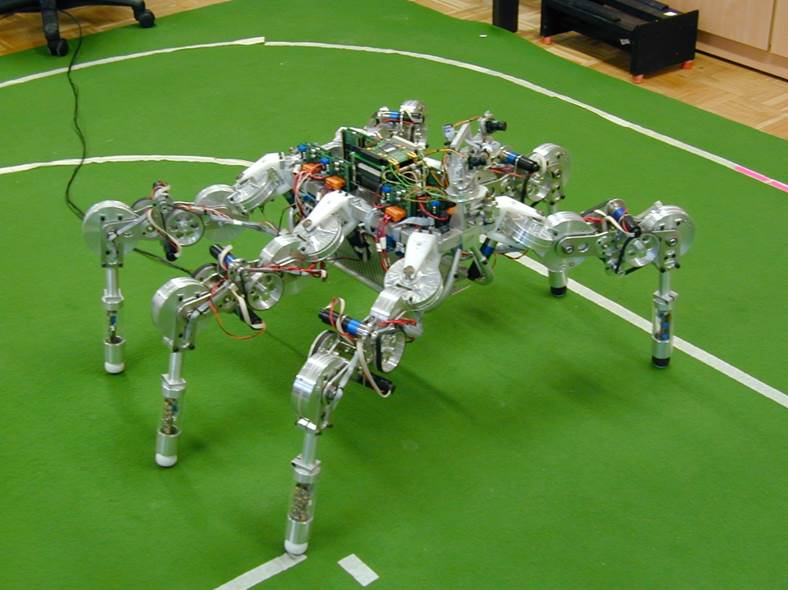
\includegraphics[width=6cm]{kapitel2/lauron3}
    \subcaption{Lauron III}\label{kap2:lauron3}
  \end{subfigure}%
  \qquad
  \begin{subfigure}[b]{.4\linewidth}
    \centering
    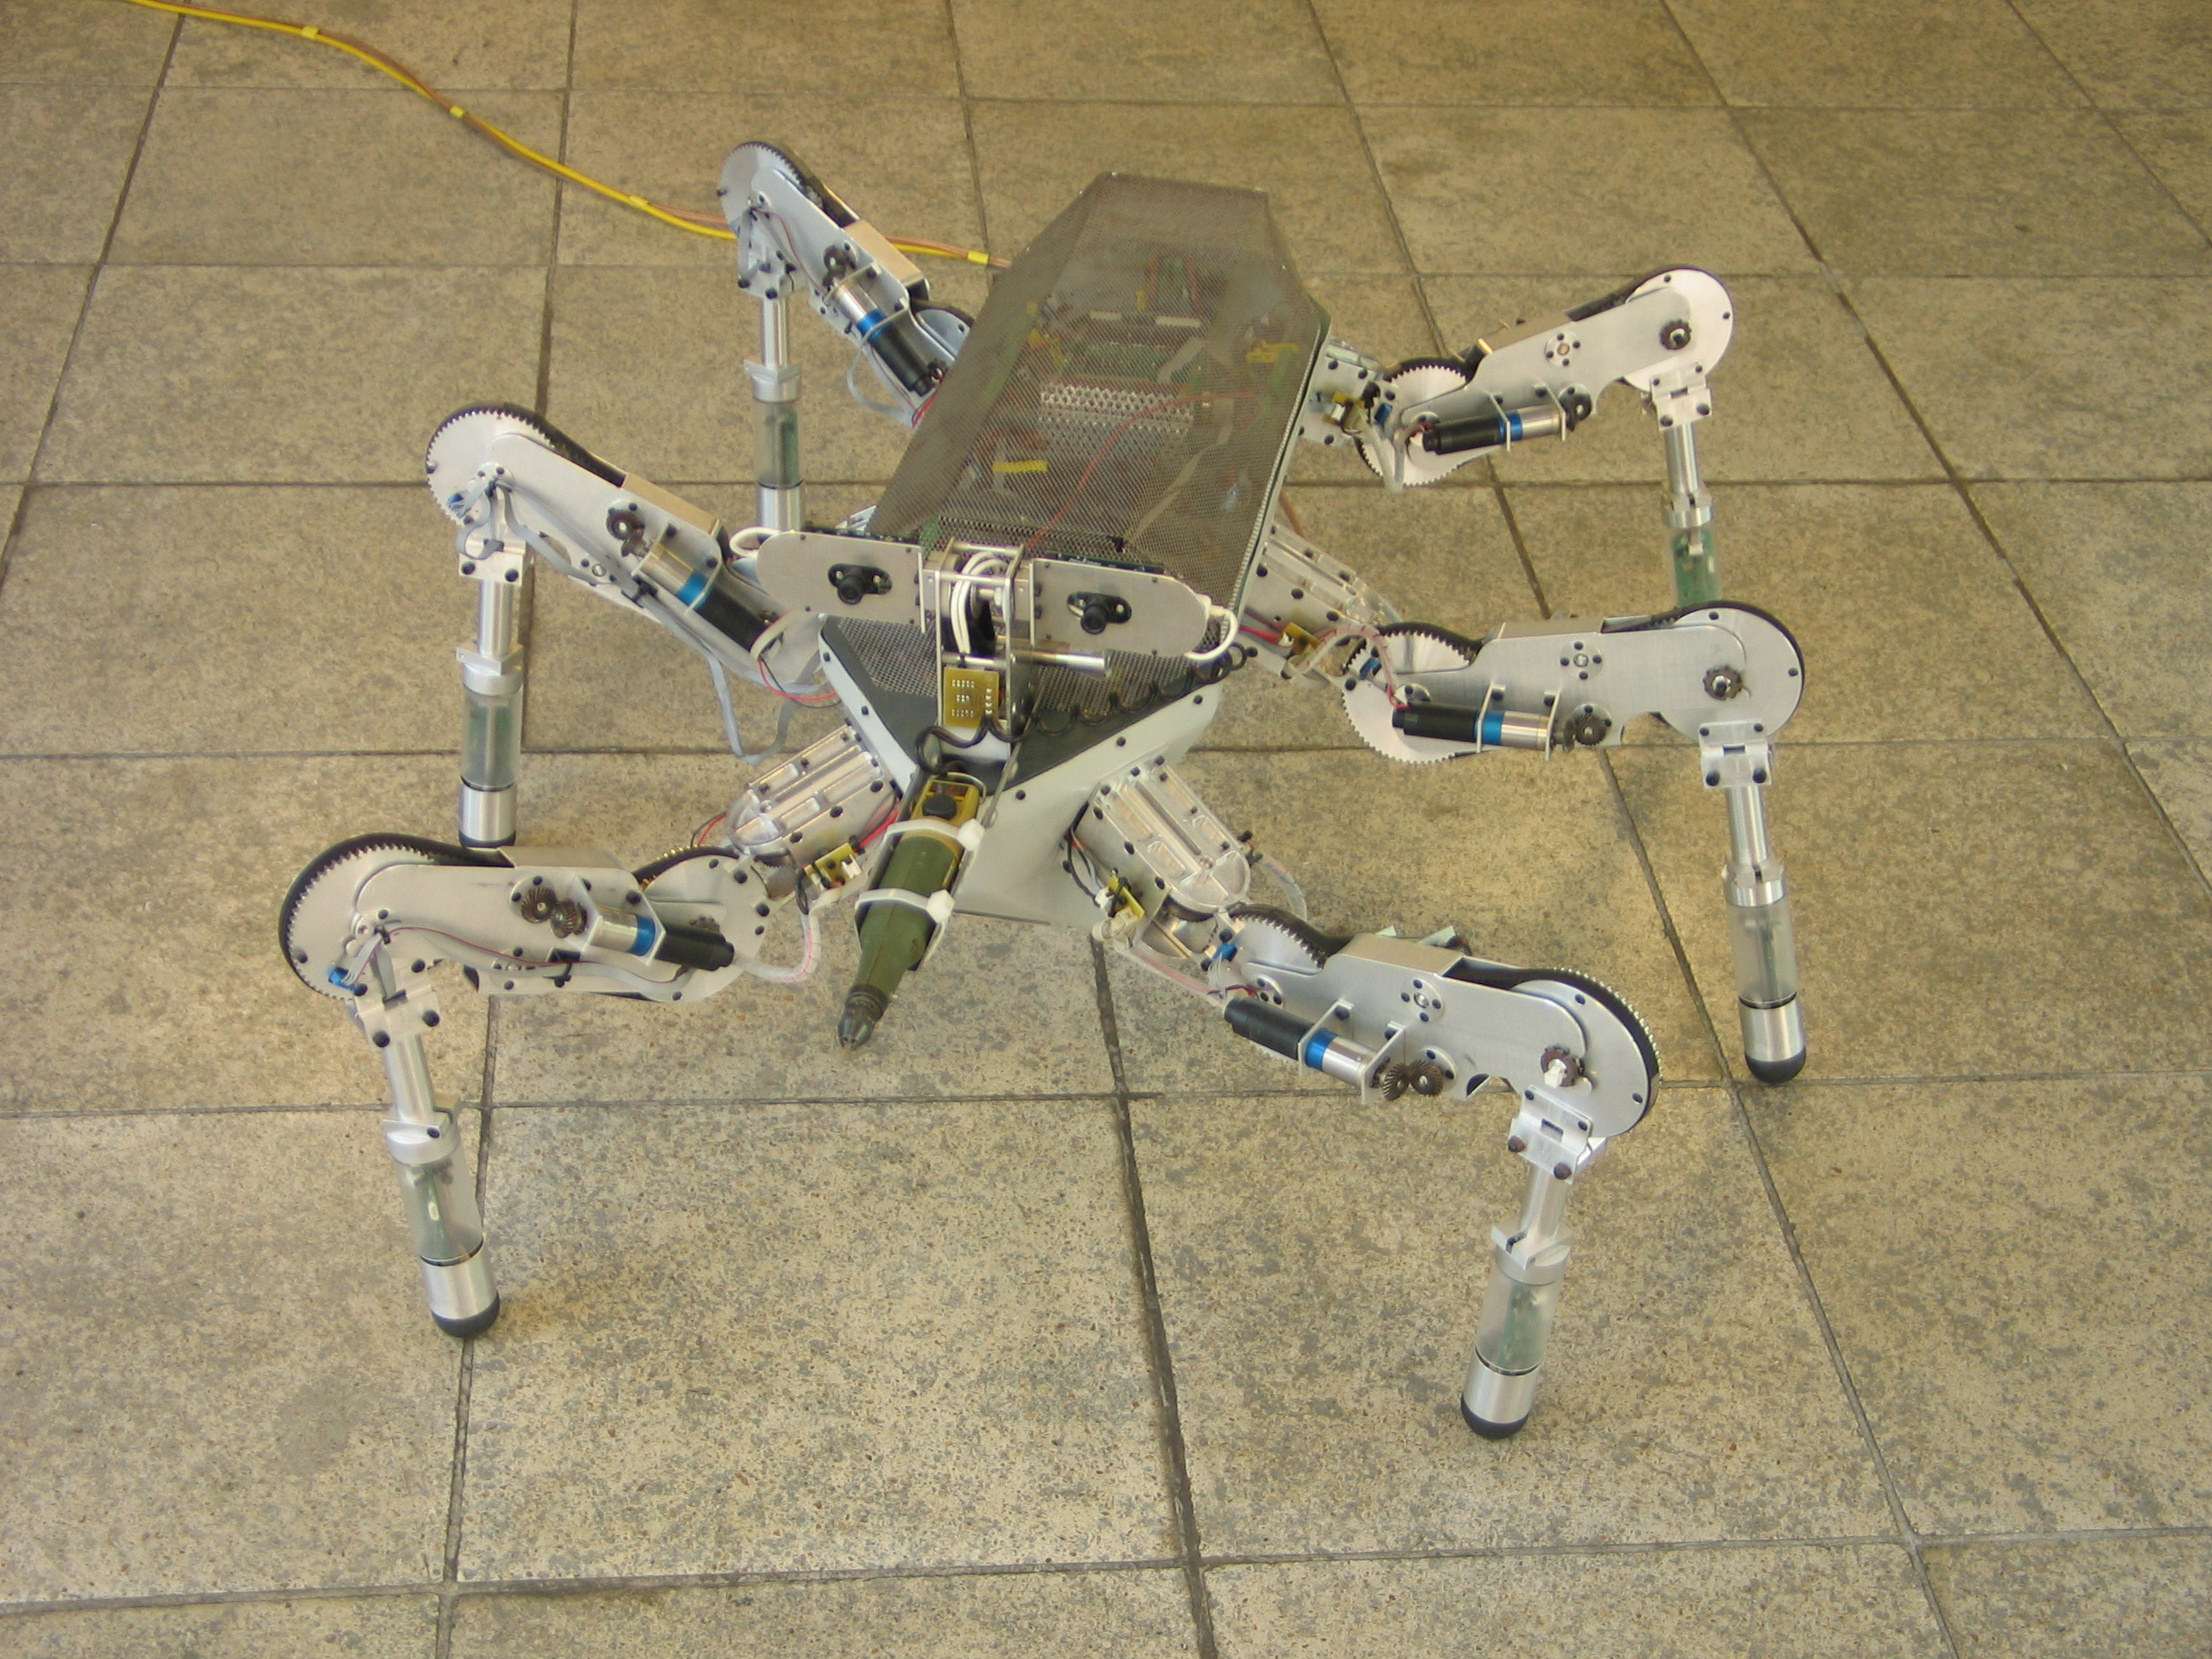
\includegraphics[width=6cm]{kapitel2/lauronivb}
    \subcaption{Lauron IVb}\label{kap2:lauron4b}
  \end{subfigure}\\
  \caption{Verschiedene Versionen des Lauron}
  \label{kap2lauron}
\end{figure}

Der Lauron basiert auf dem Vorbild der indischen Stabheuschrecke (Carausius morosus), die sehr gut erforscht ist. Dies gilt sowohl für den mechanischen Aufbau als auch für die Abläufe der Bewegungen des Roboters. Der Körper ist in drei Teile geteilt.
\begin{itemize}
  \item Kopf (Caput)
  \item Brust (Thorax)
  \item Hinterleib (Abdomen)
\end{itemize}

Die Brust ist wiederum in weitere drei Teile für jeweils ein Beinpaar unterteilt. Damit ergeben sich sechs Beine. Ein Bein besteht aus drei Segmenten:
\begin{itemize}
  \item Hüfte (Coxa)
  \item Oberschenkel (Femur)
  \item Unterschenkel (Tibia)
\end{itemize}

Die Segmente sind durch die Gelenke Subcoxal, Coxa-Trochanter und Femur-Tibia verbunden. Der Fuß jedes Beines wird Tarsus genannt. Das erste Gelenk Subcoxal besitzt zwei Freiheitsgrade, die weiteren Gelenke besitzen einen Freiheitsgrad. Damit ist für die indische Stabheuschrecke die minimale erforderliche Zahl an Freiheitsgraden erreicht, damit der Fuß beliebig im dreidimensionalen Raum gesetzt werden kann.

Unter anderem ist noch wichtig, dass der Kopf der indischen Stabheuschrecke zwei lange Fühler besitzt. Diese könnten in einem Roboter beispielsweise als Laserscanner oder Kamera modelliert werden, welche sich einen Überblick über die Gegend verschaffen können.

Der Körper des \emph{Lauron III} trägt die 7 Mikrocontroller (Infineon C167) und einen Hauptrechner, der auf Pentium basiert, die Akkumulatoren sowie den Kamerakopf. An beiden Seiten des Körpers sind jeweils drei Beine angebracht. Der Roboter wiegt 16 Kilogramm und hat eine maximale Zuladung von etwa \SI{15}{\kilo\gram}. Die Maximalgeschwindigkeit beträgt \SI{0.5}{\metre\per\second}.

\subsection{Akrobat}

Der folgende Unterabschnitt stellt den Laufroboter \emph{Akrobat} vor und nutzt dazu die Arbeit von Wilen Askerow. \autocite{askerow2014}

Auch der \emph{Akrobat} (\autoref{Kap2:akrobat}) ist der Form einer Stabheuschrecke nachempfunden und ähnelt in vielerlei Hinsicht dem Lauron. Der Roboterkörper ist ungefähr 56 Millimeter hoch, 102 Millimeter breit und hat eine Seitenlänge von 62 Millimeter. Ebenfalls besitzt dieser sechs Beine mit je drei Segmenten. Diese haben die Längen 72 Millimeter, 97 Millimeter und 163 Millimeter, welche für kinematische Berechnungen von großer Bedeutung sind. Jedes Bein wiegt ungefähr 0,8 Kilogramm.

Jedes der Gelenke hat exakt einen Freiheitsgrad, sodass das gesamte Bein drei Freiheitsgrade hat. Wie auch beim Lauron ermöglicht dies die beliebige Positionierung im dreidimensionalen Raum. Die Gelenke sind mit dem Servomotor Dynamixel RX64 ausgestattet. Außerdem hat jedes Gelenk einen definierten Arbeitsbereich, welcher nicht unter- oder überschritten werden darf.
\begin{itemize}
  \item $\alpha=\SIrange{-50}{50}{^\circ}$
  \item $\beta=\SIrange{-106}{106}{^\circ}$
  \item $\gamma=\SIrange{-135}{135}{^\circ}$
\end{itemize}  

Außerdem besitzt der Roboter am Kopf eine fest verbaute Kamera. Der Roboterkörper verfügt über genügend Freiraum für Batterien im mittleren Gehäuse. Im hinteren Gehäuse ist der Steuerrechner sowie die restliche Elektronik platziert.

\begin{figure}[b!]
  \centering
  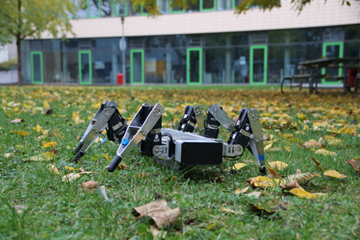
\includegraphics[height=8cm]{kapitel2/akrobat}
  \caption{Der Akrobat vor dem C-Gebäude der Hochschule Mannheim}
  \label{Kap2:akrobat}
\end{figure}

Es handelt sich beim Rechner um den Einplatinencomputer Raspberry Pi (Modell B+) mit \SI{512}{MB} Arbeitsspeicher und einem \SI{700}{MHz} ARM 11 Prozessor. Der Raspberry Pi bietet vielfältige Anschlussmöglichkeiten:
\begin{itemize}
\item Wireless Local Area Network (WLAN)
\item 4 Universal Serial Bus (USB)-Anschlüsse
\item 1 Ethernet-Anschluss
\item 1 High Definition Multimedia Interface (HDMI)-Anschluss, über den die Visualisierung mittels eines externen Bildschirms stattfindet
\item Camera Serial Interface (CSI)-Schnittstelle für die Kamera
\item Low Voltage Differential Signaling (LVDS)-Anschluss für die Ansteuerung von LCD-Displays
\item GPIO (General Purpose Input Output)-Anschlüsse
\end{itemize}

Es besteht die Möglichkeit, das Gamepad F710 von Logitech per WLAN anzuschließen. Theoretisch sind auch andere Gamepads möglich, sofern diese im Quellcode konfiguriert wurden.

\section{Kinematik}

Um dem Roboter die richtigen Befehle zu senden, müssen als nächstes die Grundlagen für die Kinematik gesetzt werden. Ein Roboterbein entspricht jeweils einer kinematischen Kette, die aus mehreren starren Körpern besteht und die über Gelenke verbunden sind. Es handelt sich sowohl beim Lauron als auch beim Akrobat um Rotationsgelenke. Dieser Abschnitt beschreibt Methoden der Kinematik.

Mit Hilfe der direkten Kinematik lässt sich auf Grund der Gelenkausrichtungen berechnen, an welcher Position sich der sogenannte Endeffektor befindet. Der Endeffektor entspricht dem Fuß des Roboters. Über die inverse Kinematik kann bei einer gegebenen Fußposition berechnet werden, wie die Fußgelenke gestellt werden sollen. Die beschriebenen Methoden wurden bereits in weiterer Literatur erläutert. \autocite{den55, wloka92, ihme02, fellmann2007}

\subsection{Denavit-Hartenberg-Verfahren}

Denavit und Hartenberg entwickelten ein Verfahren zur Beschreibung von kinematischen Ketten. Durch dieses Verfahren können mit Hilfe von nur vier Parametern, den DH-Parametern, die gegenseitige Lage zweier Elemente beschrieben werden. Dies macht die Berechnung von kinematischen Ketten wesentlich einfacher.

\begin{figure}[b!]
  \centering
  \begin{subfigure}[b]{.4\linewidth}
    \centering
    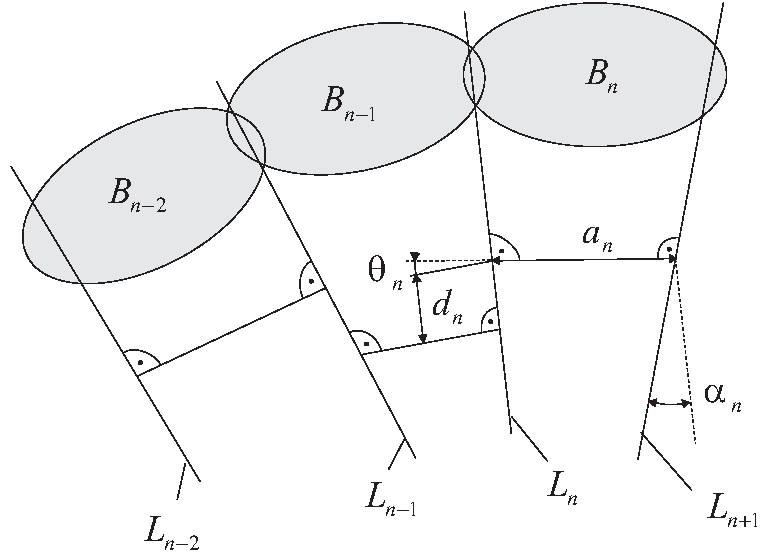
\includegraphics[width=6cm]{kapitel2/dh-parameter}
    \subcaption{Parameter}\label{kap2:dhparams}
  \end{subfigure}%
  \qquad
  \begin{subfigure}[b]{.4\linewidth}
    \centering
    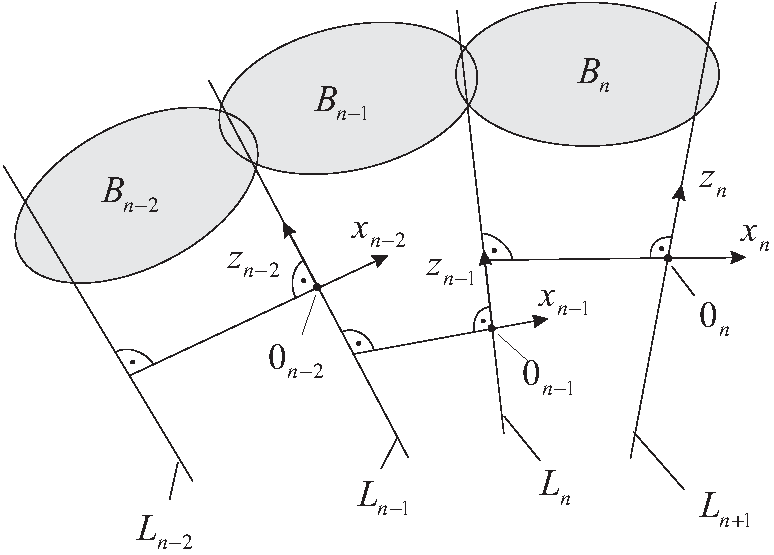
\includegraphics[width=6cm]{kapitel2/dh-koordinaten}
    \subcaption{Koordinatensysteme}\label{kap2:dhcoords}
  \end{subfigure}\\
  \caption{Denavit-Hartenberg Verfahren}
  \label{kap2lauron}
\end{figure}

Die vier Parameter (\autoref{kap2:dhparams}) können wie folgt berechnet werden:
\begin{enumerate}
  \item Entspricht der Länge der gemeinsamen Normale zwischen den Achsen $L_n$ und $L_{n+1}$. Dies ist im Schaubild die Variable $a_n$.
  \item Entspricht dem Versatz zwischen dieser und der vorherigen Normalen. Im Schaubild ist das die Variable $d_n$.
  \item Entspricht dem Drehwinkel zwischen $L_n$ und $L_{n+1}$. Im Schaubild ist das die Variable $\alpha_n$.
  \item Entspricht der Drehung um die Achse $L_n$. Im Schaubild ist dies die Variable $\theta_n$.
\end{enumerate} 

Des Weiteren ist es eine Voraussetzung für das Verfahren, dass für jedes Gelenk ein eigenes Koordinatensystem definiert ist (\autoref{kap2:dhcoords}), damit die Transformationsgleichungen aufgestellt werden können. Dabei ist es wichtig, dass eine Achse des Koordinatensystems auf der Gelenkachse und eine zweite auf der Normalen liegt. Damit sind nun alle Anforderungen erfüllt, um die direkte und die inverse Kinematik effizient zu berechnen.

\subsection{Direkte Kinematik}

\begin{figure}[b!]
  \centering
  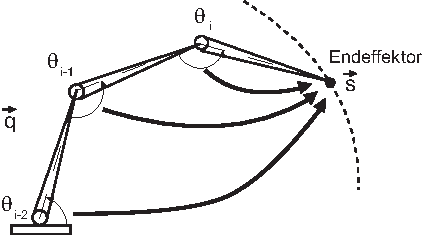
\includegraphics[height=5cm]{kapitel2/DirekteKinematik}
  \caption{Direkte Kinematik}
  \label{Kap2:direktekinematik}
\end{figure}

Mit Hilfe der direkten Kinematik lässt sich nun berechnen, an welcher Position sich der sogenannte Endeffektor befindet (\autoref{Kap2:direktekinematik}). Gegeben sind hierbei die Winkel der Gelenke. Der Vektor $ \vec{s} = (x,y,z,\alpha,\beta,\gamma)^T $  entspricht der Position und der Orientierung des Endeffektors. Der Vektor $ \vec{q} = (q_1, ...,q_n)^T $, bei dem $n$ die Anzahl der Gelenke ist, entspricht den Gelenkvariablen. Dann lässt sich die direkte Kinematik wie in \autoref{dk1} ausdrücken.
\begin{equation}
  \vec{s} = f(\vec{q})
\label{dk1}
\end{equation}

Mittels der DH-Parameter aus dem vorherigen Kapitel lässt sich nun eine homogene Transformationsmatrix vom Ausgangskoordinatensystem in das Koordinatensystem des Endeffektors abhängig der Gelenkvariablen, siehe \autoref{dk2}, erstellen.
\begin{equation}
  ^{n-1}_{n}T = \textrm{rot}(z_{n-1},\theta_n) \cdot \textrm{trans}(0,0,d_{n}) \cdot \textrm{trans}(a_{n},0,0) \cdot \textrm{rot}(x_{n},\alpha_{n})
\label{dk2}
\end{equation}

Der erste Parameter der Rotationsfunktion \textsc{rot} bestimmt die Rotationsachse. Der zweite Parameter bestimmt den Winkel. Die Funktion \textsc{trans} entspricht einer Verschiebung im Raum. Die Gleichung setzt voraus, dass die Wahl der Koordinatensysteme wie im vorherigen Kapitel beschrieben, eingehalten wird.

Als nächstes ersetzt man die Transformationen und Rotationen in \autoref{dk2} durch ihre homogenen Transformationenmatrizen und berechnet die gesamte Transformationsmatrix. Es ergibt sich das Ergebnis in \autoref{dk3} und \ref{dk3-2}, welche den Übergang vom Gelenk $n - 1$ in das Gelenk $n$ mit Hilfe der DH-Paramter beschreibt.
\begin{equation}
  ^{n-1}_{n}T = \begin{pmatrix}
    \textrm{cos}\: \theta_n & -\textrm{sin}\: \theta_n  & 0 & 0\\ 
    \textrm{sin}\: \theta_n & \textrm{cos}\: \theta_n   & 0 & 0\\ 
    0             & 0               & 1 & 0\\ 
    0             & 0               & 0 & 1\\
\end{pmatrix} \cdot
\begin{pmatrix}
  1 & 0 & 0 & a_n\\ 
  0 & 1 & 0 & 0\\ 
  0 & 0 & 1 & d_n\\ 
  0 & 0 & 0 & 1\\
\end{pmatrix} \cdot \begin{pmatrix}
  1 & 0 & 0 & 0\\ 
  0 & \textrm{cos}\: \alpha_n & -\textrm{sin}\: \alpha_n & 0\\ 
  0 & \textrm{sin}\: \alpha_n & \textrm{cos}\: \alpha_n & 0\\ 
  0 & 0 & 0 & 1\\
\end{pmatrix}
\label{dk3}
\end{equation}

\begin{equation}
^{n-1}_{n}T = \begin{pmatrix}
  \textrm{cos}\: \theta_n  & -\textrm{sin}\: \theta_n\; \textrm{cos}\: \alpha_n    & \textrm{sin}\: \theta_n\; \textrm{sin}\: \alpha_n & a_n\: \textrm{cos}\: \theta_n\\ 
  \textrm{sin}\: \theta_n  & \textrm{cos}\: \theta_n\; \textrm{cos}\: \alpha_n     & -\textrm{cos}\: \theta_n\; \textrm{sin}\: \alpha_n & a_n\: \textrm{sin}\: \theta_n\\ 
  0               & \textrm{sin}\: \alpha_n                & \textrm{cos}\: \alpha_n & d_n\\ 
  0               & 0                             & 0 & 1\\
\end{pmatrix}
\label{dk3-2}
\end{equation}

Da dies nur die Transformation zwischen einem und dem vorherigen Gelenk berechnet, muss nun die gesamte kinematische Kette in \autoref{dk4} hergestellt werden. Dies erfolgt durch die Multiplikation aller Einzeltransformationen.
\begin{equation}
  ^{0}_{m}T =\: ^{0}_{1}T \cdot \: ^{1}_{2}T \cdot \: ...\: ^{m-1}_{m}T
\label{dk4}
\end{equation}

Mit dieser Matrix kann ein Punkt im Koordinatensystem des Endeffektors in das Anfangskoordinatensystem transformiert werden. Ebenfalls lässt sich durch eine Aufteilung in Teilmatrizen die Orientierung und Position des Endeffektors relativ zum Anfangskoordinatensystem berechnen. Dazu dient \autoref{dk5}.
\begin{equation}
  _{m}^{0}T = \begin{pmatrix}
    _{m}^{0}R & ^{0}\vec{r}\\
    0 & 1\\
  \end{pmatrix}
\label{dk5}
\end{equation}

Dabei ist der Vektor $^{0}\vec{r}$ der gesuchte Vektor vom Koordinatensystem zum Endeffektor. Mit Hilfe der 3x3 Rotationsmatrix $\,_{m}^{0}R$, welche die Orientierung dieser Transformationen angibt, können die Winkel des Endeffektors berechnet werden. Dazu wird die Matrix noch aufgelöst. Durch das Auflösen des Gleichungssystems ergeben sich schlussendlich die folgenden Winkel in \autoref{dk6}:

\begin{equation}
  \begin{aligned}
    \alpha & = \arctan{(\frac{\alpha_{21}}{\alpha_{11}})} \\[1em]
    \beta & = \arctan{(\frac{-\alpha_{31}}{\alpha_{11} \cos{\gamma} + \alpha_{21} \sin{\gamma}})} \\[1em]
    \gamma & = \arctan{(\frac{\alpha_{32}}{\alpha_{33}})}
  \end{aligned}
  \label{dk6}
\end{equation}

\subsection{Inverse Kinematik}

\begin{figure}[b!]
  \centering
  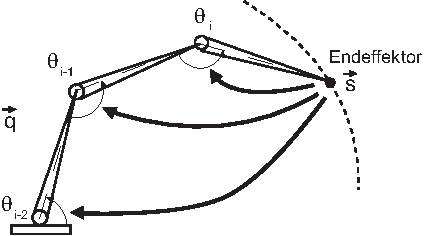
\includegraphics[height=5cm]{kapitel2/InverseKinematik}
  \caption{Inverse Kinematik}
  \label{Kap2:inversekinematik}
\end{figure}

Mit Hilfe der inversen Kinematik lässt sich nun berechnen, wie die Gelenkswinkel ausgerichtet werden müssen, damit der Endeffektor an eine bestimmte Position kommt (\autoref{Kap2:inversekinematik}). Dies ist gleichbedeutend mit der inversen Funktion der direkten Kinematik (\autoref{ik1}).
\begin{equation}
  \vec{q} = f^{-1}(\vec{s})
\label{ik1}
\end{equation}

Dabei ist zu beachten, dass es in den meisten Fällen für eine Eingabe mehrere Lösungen geben kann. Eine berechnete Lösung kann aber auch ungültig sein, wenn beispielsweise der Arbeitsbereich eingeschränkt ist oder Hindernisse auf dem Weg zur gewünschten Position liegen. Ebenfalls gibt es für viele Positionen auch gar keine Lösung. Des Weiteren kann die kinematische Kette durch Singularitäten Freiheitsgrade verlieren. Dies geschieht, wenn die Drehung an unterschiedlichen Achsen dieselbe Bewegung ergibt, dadurch, dass diese aufeinander liegen oder parallel verlaufen.

Da bereits die Funktion der direkten Kinematik eine nichtlineare Funktion ist, ist auch die inverse Funktion eine nichtlineare Funktion. Das Problem gehört damit in die Kategorie der Lösung eines nichtlinearen Gleichungssystems. Dies lässt sich über eine analytisches Verfahren oder annähernd über ein numerisches Verfahren lösen.

Bei der analytischen Methode wird versucht, auf Basis der geometrischen Eigenschaften eine Formel herzuleiten. Dies wird umso schwerer, je mehr Freiheitsgrade die kinematische Kette hat. Der Vorteil liegt darin, dass die analytische Lösung ersten alle möglichen Gelenkstellungen für eine Position liefert und zweitens, dass sie wesentlich performanter ist. Die Lösungen sind exakt und Singularitäten können bereits beim Aufstellen der Gleichung festgestellt werden.

Die Software \emph{ikfast} \autocite{diankov2010ikfast} findet Lösungen und erstellt Gleichungen für die inverse Kinematik einer kinematischen Kette. Dabei nutzt die Software im Gegensatz zu anderer Software statt der numerischen die analytische Methode.

Bei der numerischen Lösung wird mittels einer linearen Annäherung versucht die Lösung für $f^{-1}$ zu finden. Dies lässt sich mit der Jacobi-Matrix berechnen. Dazu werden Teilfunktionen für $x$, $y$, $z$, $\alpha$, $\beta$ und $\gamma$ benötigt, welche sich aus der Transformationsmatrix der direkten Kinematik ergeben. Die Teilfunktionen werden dann nach jeder Variablen partiell abgeleitet. Dies ergibt die $6\,x\,n$ Jacobi-Matrix. Sie beschreibt die Änderung der Position des Endeffektors bei Änderung der Gelenkstellungen.

Durch weitere Umstellung der Funktion ergibt sich eine Gleichung für die lineare Annäherung an die gewünschte Funktion. Diese Lösung wird dann mittels direkter Kinematik überprüft. Ist die Abweichung zu groß, wird die Jacobi-Matrix mit den zuvor berechneten Gelenkstellungen erneut berechnet. Dies ergibt die lineare Annäherung an die Lösung. Wichtig ist dabei, dass eine maximale Zahl an Iterationen für den Algorithmus angegeben ist, da es manchmal auch gar keine Lösung geben kann.

Im Gegensatz zur analytischen Methode liefert die numerische Lösung immer nur einen Wert. Ein weiteres Problem der numerischen Lösung sind Singularitäten, welche auftreten können, wenn die Jacobi-Matrix an Rang verliert und somit singulär wird. Die Folge ist, dass die Matrix nicht mehr invertierbar ist und damit keine Lösung mehr berechnet werden kann.

TODO START:
Hier bitte überlegen, ob die Formeln für die analytische Lösung gezeigt werden können. Für Akrobat und meine Diss ist das grundsätzlich gleich. Ich empfehle die Formeln von Wilen. 
TODO END

\section{Laufplanung}

Nun werden die Grundlagen für die Laufplanung dargestellt. Dazu werden verschiedene reguläre Laufmuster und das freie Laufmuster Random Sampling dargestellt. Die regulären Laufmuster wurden in zahlreicher Literatur bei vielen Insekten beobachtet und auf das Thema Robotik übertragen. \autocite{ferrell1995comparison, wilson1966insect}

In der Robotik eignen sich diese, um auf ebenem Grund voranzuschreiten. Allerdings gibt es auch Untergründe, die stark uneben sind oder unüberwindbare Hindernisse aufweisen. Dann können freie Laufmuster wie Random Sampling zum Einsatz kommen.

\subsection{Reguläre Laufmuster}

Bei den regulären Laufmustern unterscheidet man zwischen drei häufig bei Insekten beobachteten Laufmustern, die aber alle der Gruppe \emph{wave gait} angehören:
\begin{itemize}
\item slow wave gait
\item ripple gait
\item tripod gait
\end{itemize}

Zunächst einmal müssen zwei Begriffe definiert werden, welche für die Betrachtung der Laufmuster wichtig sind. Diese entsprechen den beiden Phasen, welche die freien Laufmuster benötigen, um nach vorne zu laufen.
\begin{itemize}
\item \emph{power stroke}: In dieser Phase steht das Bein auf dem Boden und unterstützt die Körpermitte, sich nach vorne zu bewegen. Damit die Körpermitte sich nach vorne bewegen kann, wird das Bein in die entgegengesetzte Richtung gezogen, während es auf dem Boden bleibt.
\item \emph{return stroke}: Das Bein wird angehoben und nach vorne auf die nächste Position für die Ausführung der \emph{power stroke} gesetzt.
\end{itemize}

\begin{figure}[b!]
  \centering
  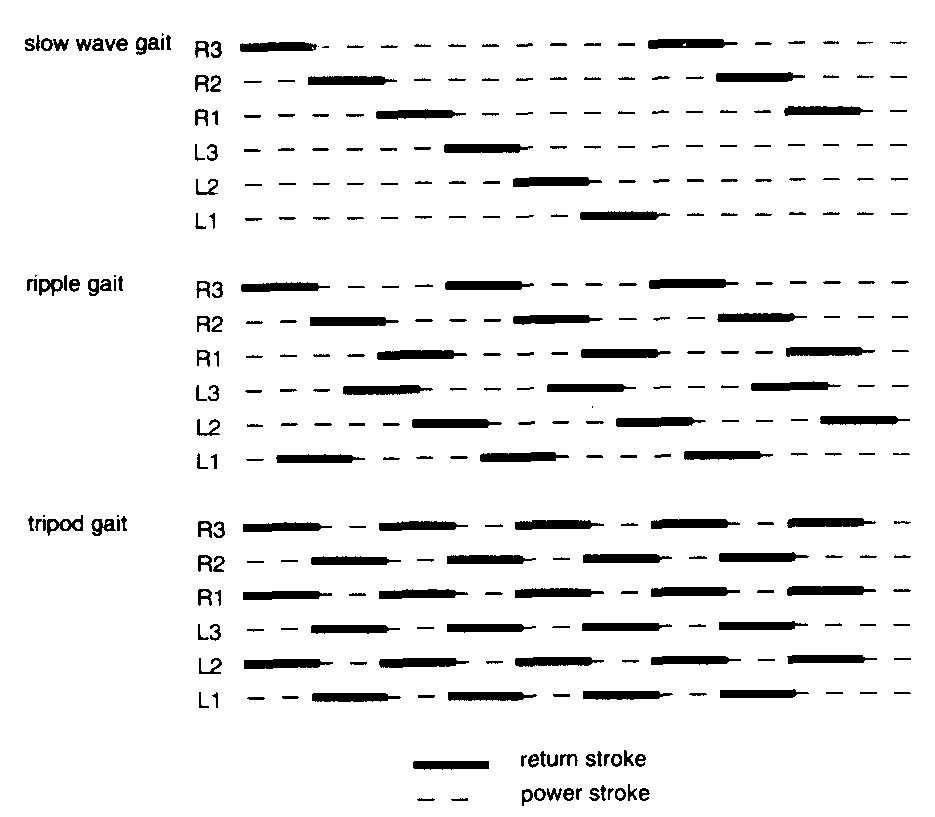
\includegraphics[height=8cm]{kapitel2/freie-gangarten}
  \caption[Reguläre Laufmuster von Insekten]{Reguläre Laufmuster von Insekten \autocite{ferrell1995comparison} \autocite{wilson1966insect}}
  \label{Kap2:laufmuster}
\end{figure}

\autoref{Kap2:laufmuster} zeigt nun für die drei Laufmuster zeitlich dargestellt, wann die \emph{power stroke} und wann die \emph{return stroke} ausgeführt wird.

Beim \emph{slow wave gait} befindet sich immer ein Bein in der \emph{return stroke}, während alle anderen sich in der \emph{power stroke} befinden und den Roboterkörper stützen und nach vorne bewegen. Auch die Reihenfolge spielt eine Rolle. Zuerst werden alle Beine einer Seite umgesetzt, dann erst alle der anderen Seite.

Beim \emph{ripple gait} werden um eine drittel Phase verschoben die Beine nacheinander umgesetzt. Daraus ergibt sich eine schnellere Bewegung als beim \emph{slow wave gait}. Auch hier spielt die Reihenfolge eine Rolle. Es wird immer abwechselnd ein Bein von links und dann ein Bein von rechts umgesetzt, während die anderen Beine in der \emph{power stroke} den Roboterkörper stützen und nach vorne bewegen.

Beim \emph{tripod gait} sind gleichzeitig drei Beine in der Phase \emph{power stroke}, während drei Beine in der Phase \emph{return stroke} sind. Bei der Auswahl müssen zwei Beine der einen Seite und ein Bein der anderen Seite ausgewählt werden, damit der Roboter nicht umfällt.

Da der \emph{tripod gait} die Phasen am schnellsten durchläuft, weil er immer die maximale Anzahl an möglichen Beinen gleichzeitig umsetzt oder stützen lässt, ist er in diesem Umfeld auch das schnellste der drei Laufmuster. Etwas langsamer ist der \emph{ripple gait}, während der \emph{slow wave gait} am langsamsten ist, da die Beine immer nur nacheinander umgesetzt werden.

\subsection{Freie Laufmuster}

Nun wird das freie Laufmuster \emph{Random Sampling} sowie einige weitere relevante Algorithmen vorgestellt. \autocite{herms2004}


\subsubsection{Random Sampling}

Beim Random Sampling werden zufällige gültige Lösungen generiert.  Wichtig ist, dass alle möglichen Lösungen generiert werden können und nur Lösungen ausgeschlossen werden, die außerhalb des gültigen Bereichs der Fußwinkel und Fußgeschwindigkeiten liegen, die auf instabilem Untergrund wie einem zu starkem Gefälle liegen oder die den Roboter zum Umkippen bringen würden.

Das Generieren von Lösungen erfolgt nun in mehreren Schritten. Zu Beginn müssen einige Berechnungen für die Festlegung des Pfades zum Ziel ablaufen, bevor der Hauptteil des Algorithmus abläuft, welcher sich schrittweise an das Ziel nähert, bis der Abstand zum Ziel annähernd null beträgt.

\paragraph{Festlegung des Pfades zum Ziel}

Eine erste Methode ist es, den Weg vom Start zum Ziel auf direktem Weg zu erreichen. Da allerdings nicht immer Lösungen auf direktem Weg möglich sind, müssen auch andere Pfade generiert werden. Beispielsweise könnte ein unüberwindbarer Graben oder eine hohe Mauer dafür sorgen, dass kein direkter Weg möglich ist. In diesem Fall müsste der Laufroboter den Weg um das Hindernis planen, um eine gültige Lösung zu finden. Um nun alle Fälle abzudecken, benötigt man eine zufällige Streckenplanung. Diese erfolgt, indem zuerst die Anzahl der Pfadsegmente festgelegt wird und dann genau so viele Wegpunkte gesetzt werden.

\paragraph{Festlegung der Anzahl der Pfadsegmente}

Die Festlegung der Anzahl der Pfadsegmente erfolgt über eine \emph{geometrische Verteilung}. Diese Verteilung wird genutzt, da eine geringe Anzahl an Pfadsegmenten häufig sein sollen, da davon ausgangen wird, dass der direkte Weg der schnellste Weg ist. Höhere Anzahlen an Pfadsegmenten sollen weniger oft auftreten. Durch die Veränderung des Parameters $p$ lassen sich die Wahrscheinlichkeiten dahingehend variieren, dass entweder eine höhere oder eine niedrigere Anzahl an Pfadsegmenten bevorzugt werden. Standardmäßig geht man von p=\SI{0.5}{} aus, welches die Wahrscheinlichkeitsverteilung in \autoref{Kap3:streckenabschnittWahrscheinlichkeit} ergibt.

\begin{table}[t]
  \caption{Wahrscheinlichkeit der Anzahl der Pfadsegmente für die geplante Strecke}
  \label{Kap3:streckenabschnittWahrscheinlichkeit}
  \centering
  \sffamily
  \begin{footnotesize}
    \begin{tabular}{c S[table-format=1.3,table-comparator=true,table-space-text-post={***}]}
    \toprule
    \textbf{Pfadsegmente} & \textbf{Wahrscheinlichkeit $[\%]$}\\
    \midrule
    1 & 50,0\\
    2 & 25,0\\
    3 & 12,5\\
    4 & 6,25\\
    5 & 3,125\\
    \bottomrule
    \end{tabular}
  \end{footnotesize}
  \rmfamily
\end{table}

\paragraph{Festlegung der Wegpunkte}

Nachdem die Anzahl der Pfadsegmente definiert ist, müssen nun die Koordinaten der Wegpunkte zufällig generiert werden. Für jeden Pfadpunkt $P$ wird einzeln eine Lösung generiert. Zunächst wird der Mittelpunkt $m(x, y)$ sowie die Länge $l$ zwischen Start und Ende berechnet. Auf den Mittelpunkt wird nun ein zufälliger Vektor $r(x, y)$ addiert, dessen generierter Wert vom negativen bis zum positiven Betrag der Länge $l$ reicht. \autoref{RandomSamplingWegpunkteP1} und \autoref{RandomSamplingWegpunkteP2} zeigen mögliche Ergebnisse für drei Pfadsegmente $P_1$, $P_2$ und $P_3$ für den Startpunkt $S(0,0)$ und dem Zielpunkt $Z(10,0)$. Der letzte Pfadpunkt $P_3$ entspricht immer genau der Zielposition, damit der Roboter dieses Ziel in jedem Fall erreicht. \autoref{Kap2:RSWegpunkte} zeigt die generierten Punkte und damit den Pfad des Roboters grafisch dargestellt.

\begin{align}
\label{RandomSamplingWegpunkteP1} P_1&=\left(\begin{array}{c} x_m + x_r \\ y_m + y_r \end{array}\right)=\left(\begin{array}{c} 5 - 2.31 \\ 0 - 4.1 \end{array}\right)=\left(\begin{array}{c} 3.31 \\ -4.1 \end{array}\right) \\[1em]
\label{RandomSamplingWegpunkteP2} P_2&=\left(\begin{array}{c} x_m + x_r \\ y_m + y_r \end{array}\right)=\left(\begin{array}{c} 5 + 3.1 \\ 0 + 0.5 \end{array}\right)=\left(\begin{array}{c} 8.1 \\ 0.5 \end{array}\right)
\end{align}

\begin{figure}[t!]
  \centering
  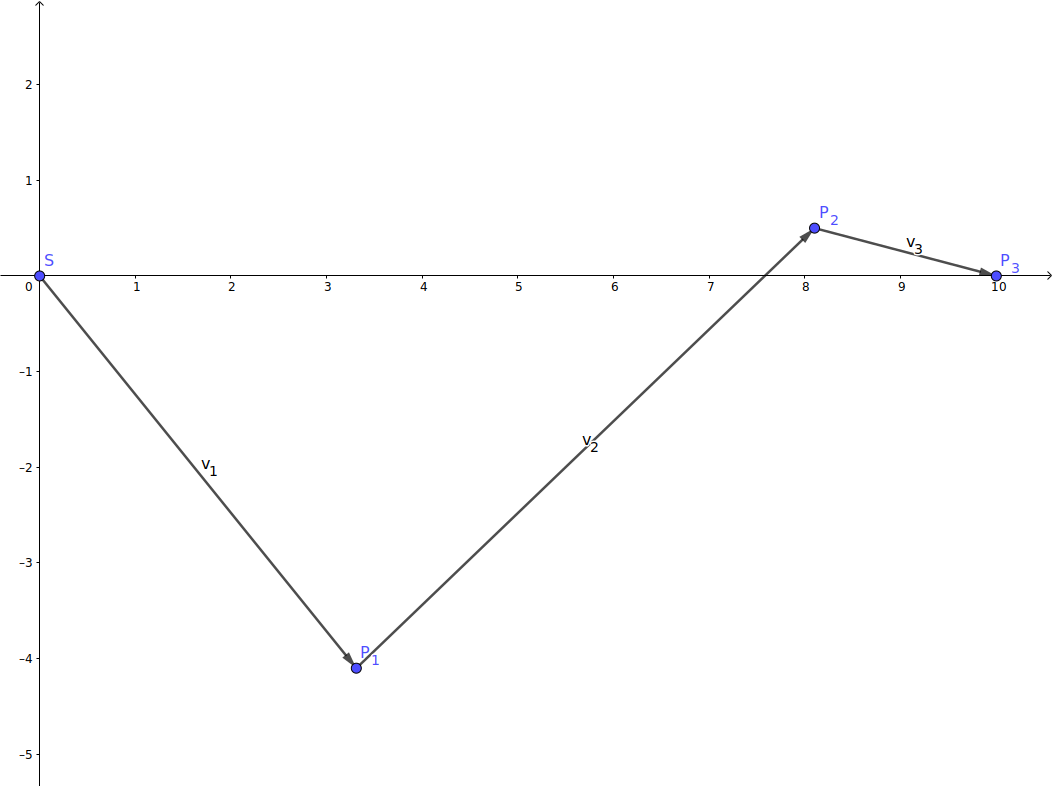
\includegraphics[width=1\textwidth]{kapitel2/rswegpunkte}
  \caption{Zufällig generierte Wegpunkte}
  \label{Kap2:RSWegpunkte}
\end{figure}

Mit dieser Berechnung sind nun für den Mittelpunkt des Körpers des Laufroboters ausschließlich Bewegungen auf diesem Pfad möglich. Bewusst wird hier noch nicht mit der $z$-Koordinate gearbeitet, da diese je nach Fußstellung und Terrain variiert.

\paragraph{Schrittweise Näherung an das Ziel}

Die schrittweise Näherung an das Ziel erfolgt solange, bis der Abstand zum Ziel minimal ist. Ein exakter Vergleich mit dem Abstand null ist nicht effektiv, da der Roboter sonst fortwährend versuchen würde auf seine Zielposition zu gelangen, aber ununterbrochen minimale Abweichungen zum Ziel hätte, was den Prozess erneut anstoßen würde. Der Ablauf, um die Füße anzuheben oder abzusetzen sowie den Körper zu bewegen, läuft folgendermaßen ab:
\begin{enumerate}
  \item Berechnung des zulässigen Bereichs
  \item Auswahl der nächsten Fuß-Konfiguration
\end{enumerate}

\paragraph{Berechnung des zulässigen Bereichs}

Der zulässige Bereich des Mittelpunkts ist auf Grund von zwei Kriterien eingeschränkt. Zum einen durch die maximalen Reichweite der Fußpunkte vom Mittelpunkt aus. Zum anderen dadurch, dass der minimale \emph{Stability Margin} nicht unterschritten werden darf. Der Stability Margin ist der kleinste Abstand zum Mittelpunkt der konvexen Hülle der Fußpunkte vom Mittelpunkt aus. Dieser ist ein Maß dafür, wie stabil der Roboter steht. Ist der Stability Margin kleiner als null, so ist der Mittelpunkt außerhalb der konvexen Hülle, was ein Kippen des Roboters verursacht. Je größer der Stability Margin, desto stabiler steht der Roboter.

Der zulässige Bereich kann nur an zwei Punkten verlassen werden. Damit wird ein Start- und ein Endpunkt der aktuellen Fußstellung gebildet. Diese sind analytisch schwer zu berechnen. Daher muss mit einem numerischen Verfahren, der \emph{binären Suche}, mit einem inneren zulässigen Punkt und einem äußerem unzulässigen Punkt der Schnittpunkt mit dem zulässigen Bereich gesucht werden. Dazu genügt eine Funktion welche angibt, ob der Mittelpunkt zulässig oder unzulässig ist.

\paragraph{Auswahl der nächsten Fuß-Konfiguration}

Der Mittelpunkt des Roboterkörpers kann sich in diesem aktuellen Zustand nur noch vom zuletzt berechneten Start- und Endpunkt des zulässigen Bereichs bewegen. Dies geschieht durch das Verschieben der Körpermitte. Dazu müssen die Füße gehoben und umgesetzt werden. Auch hier müssen die zu Beginn genannten Kriterien beachtet werden. Diese sind unter anderem, dass sich mindestens drei Füße auf dem Boden befinden und dass mindestens ein Fuß auf jeder Seite den Körper stützt, damit der Stability Margin positiv ist. Mit diesen Regeln lassen sich 40 mögliche Fußkonfigurationen, auch Stützzustände genannt, darstellen, welche in \autoref{validconf} abgebildet sind.

\begin{figure}[t!]
\setlength{\unitlength}{1.1cm}
\begin{picture}(1.5,3.5)
\put(0.25,0.25){\dashbox{0.05}(1,2){} }
\put(0.25,1.25){\circle*{0.2}}
\put(1.25,1.25){\circle*{0.2}}
\put(1.25,0.25){\circle*{0.2}}
\put(1.25,0.25){\line(0,1){1}}
\put(0.25,1.25){\line(0,0){0}}
\put(0.25,1.25){\line(1, -1){1}}
\put(0.25,1.25){\line(1, 0){1}}
\put(0.75,2.5){\makebox(0,0)[b]{1}}
\end{picture}
\begin{picture}(1.5,3.5)
\put(0.25,0.25){\dashbox{0.05}(1,2){} }
\put(0.25,1.25){\circle*{0.2}}
\put(1.25,1.25){\circle*{0.2}}
\put(0.25,0.25){\circle*{0.2}}
\put(1.25,1.25){\line(0,0){0}}
\put(0.25,0.25){\line(0,1){1}}
\put(0.25,0.25){\line(1, 1){1}}
\put(0.25,1.25){\line(1, 0){1}}
\put(0.75,2.5){\makebox(0,0)[b]{2}}
\end{picture}
\begin{picture}(1.5,3.5)
\put(0.25,0.25){\dashbox{0.05}(1,2){} }
\put(0.25,2.25){\circle*{0.2}}
\put(0.25,1.25){\circle*{0.2}}
\put(1.25,1.25){\circle*{0.2}}
\put(1.25,1.25){\line(0,0){0}}
\put(0.25,1.25){\line(0,1){1}}
\put(0.25,1.25){\line(1, 0){1}}
\put(0.25,2.25){\line(1, -1){1}}
\put(0.75,2.5){\makebox(0,0)[b]{3}}
\end{picture}
\begin{picture}(1.5,3.5)
\put(0.25,0.25){\dashbox{0.05}(1,2){} }
\put(1.25,2.25){\circle*{0.2}}
\put(0.25,1.25){\circle*{0.2}}
\put(1.25,1.25){\circle*{0.2}}
\put(1.25,1.25){\line(0,1){1}}
\put(0.25,1.25){\line(0,0){0}}
\put(0.25,1.25){\line(1, 0){1}}
\put(0.25,1.25){\line(1, 1){1}}
\put(0.75,2.5){\makebox(0,0)[b]{4}}
\end{picture}
\begin{picture}(1.5,3.5)
\put(0.25,0.25){\dashbox{0.05}(1,2){} }
\put(1.25,1.25){\circle*{0.2}}
\put(0.25,0.25){\circle*{0.2}}
\put(1.25,0.25){\circle*{0.2}}
\put(1.25,0.25){\line(0,1){1}}
\put(0.25,0.25){\line(0,0){0}}
\put(0.25,0.25){\line(1, 0){1}}
\put(0.25,0.25){\line(1, 1){1}}
\put(0.75,2.5){\makebox(0,0)[b]{5}}
\end{picture}
\begin{picture}(1.5,3.5)
\put(0.25,0.25){\dashbox{0.05}(1,2){} }
\put(0.25,1.25){\circle*{0.2}}
\put(0.25,0.25){\circle*{0.2}}
\put(1.25,0.25){\circle*{0.2}}
\put(1.25,0.25){\line(0,0){0}}
\put(0.25,0.25){\line(0,1){1}}
\put(0.25,0.25){\line(1, 0){1}}
\put(0.25,1.25){\line(1, -1){1}}
\put(0.75,2.5){\makebox(0,0)[b]{6}}
\end{picture}
\begin{picture}(1.5,3.5)
\put(0.25,0.25){\dashbox{0.05}(1,2){} }
\put(0.25,2.25){\circle*{0.2}}
\put(1.25,2.25){\circle*{0.2}}
\put(1.25,1.25){\circle*{0.2}}
\put(1.25,1.25){\line(0,1){1}}
\put(0.25,2.25){\line(0,0){0}}
\put(0.25,2.25){\line(1, -1){1}}
\put(0.25,2.25){\line(1, 0){1}}
\put(0.75,2.5){\makebox(0,0)[b]{7}}
\end{picture}
\begin{picture}(1.5,3.5)
\put(0.25,0.25){\dashbox{0.05}(1,2){} }
\put(0.25,2.25){\circle*{0.2}}
\put(1.25,2.25){\circle*{0.2}}
\put(0.25,1.25){\circle*{0.2}}
\put(1.25,2.25){\line(0,0){0}}
\put(0.25,1.25){\line(0,1){1}}
\put(0.25,1.25){\line(1, 1){1}}
\put(0.25,2.25){\line(1, 0){1}}
\put(0.75,2.5){\makebox(0,0)[b]{8}}
\end{picture}
\begin{picture}(1.5,3.5)
\put(0.25,0.25){\dashbox{0.05}(1,2){} }
\put(1.25,2.25){\circle*{0.2}}
\put(1.25,1.25){\circle*{0.2}}
\put(0.25,0.25){\circle*{0.2}}
\put(1.25,1.25){\line(0,1){1}}
\put(0.25,0.25){\line(0,0){0}}
\put(0.25,0.25){\line(1, 1){1}}
\put(0.25,0.25){\line(1, 2){1}}
\put(0.75,2.5){\makebox(0,0)[b]{9}}
\end{picture}
\begin{picture}(1.5,3.5)
\put(0.25,0.25){\dashbox{0.05}(1,2){} }
\put(1.25,2.25){\circle*{0.2}}
\put(0.25,1.25){\circle*{0.2}}
\put(0.25,0.25){\circle*{0.2}}
\put(1.25,2.25){\line(0,0){0}}
\put(0.25,0.25){\line(0,1){1}}
\put(0.25,0.25){\line(1, 2){1}}
\put(0.25,1.25){\line(1, 1){1}}
\put(0.75,2.5){\makebox(0,0)[b]{10}}
\end{picture}
\begin{picture}(1.5,3.5)
\put(0.25,0.25){\dashbox{0.05}(1,2){} }
\put(0.25,2.25){\circle*{0.2}}
\put(1.25,1.25){\circle*{0.2}}
\put(1.25,0.25){\circle*{0.2}}
\put(1.25,0.25){\line(0,1){1}}
\put(0.25,2.25){\line(0,0){0}}
\put(0.25,2.25){\line(1, -2){1}}
\put(0.25,2.25){\line(1, -1){1}}
\put(0.75,2.5){\makebox(0,0)[b]{11}}
\end{picture}
\begin{picture}(1.5,3.5)
\put(0.25,0.25){\dashbox{0.05}(1,2){} }
\put(0.25,2.25){\circle*{0.2}}
\put(0.25,1.25){\circle*{0.2}}
\put(1.25,0.25){\circle*{0.2}}
\put(1.25,0.25){\line(0,0){0}}
\put(0.25,1.25){\line(0,1){1}}
\put(0.25,1.25){\line(1, -1){1}}
\put(0.25,2.25){\line(1, -2){1}}
\put(0.75,2.5){\makebox(0,0)[b]{12}}
\end{picture}
\begin{picture}(1.5,3.5)
\put(0.25,0.25){\dashbox{0.05}(1,2){} }
\put(0.25,2.25){\circle*{0.2}}
\put(1.25,2.25){\circle*{0.2}}
\put(1.25,0.25){\circle*{0.2}}
\put(1.25,0.25){\line(0,2){2}}
\put(0.25,2.25){\line(0,0){0}}
\put(0.25,2.25){\line(1, -2){1}}
\put(0.25,2.25){\line(1, 0){1}}
\put(0.75,2.5){\makebox(0,0)[b]{13}}
\end{picture}
\begin{picture}(1.5,3.5)
\put(0.25,0.25){\dashbox{0.05}(1,2){} }
\put(1.25,2.25){\circle*{0.2}}
\put(0.25,0.25){\circle*{0.2}}
\put(1.25,0.25){\circle*{0.2}}
\put(1.25,0.25){\line(0,2){2}}
\put(0.25,0.25){\line(0,0){0}}
\put(0.25,0.25){\line(1, 0){1}}
\put(0.25,0.25){\line(1, 2){1}}
\put(0.75,2.5){\makebox(0,0)[b]{14}}
\end{picture}
\begin{picture}(1.5,3.5)
\put(0.25,0.25){\dashbox{0.05}(1,2){} }
\put(0.25,2.25){\circle*{0.2}}
\put(1.25,2.25){\circle*{0.2}}
\put(0.25,0.25){\circle*{0.2}}
\put(1.25,2.25){\line(0,0){0}}
\put(0.25,0.25){\line(0,2){2}}
\put(0.25,0.25){\line(1, 2){1}}
\put(0.25,2.25){\line(1, 0){1}}
\put(0.75,2.5){\makebox(0,0)[b]{15}}
\end{picture}
\begin{picture}(1.5,3.5)
\put(0.25,0.25){\dashbox{0.05}(1,2){} }
\put(0.25,2.25){\circle*{0.2}}
\put(0.25,0.25){\circle*{0.2}}
\put(1.25,0.25){\circle*{0.2}}
\put(1.25,0.25){\line(0,0){0}}
\put(0.25,0.25){\line(0,2){2}}
\put(0.25,0.25){\line(1, 0){1}}
\put(0.25,2.25){\line(1, -2){1}}
\put(0.75,2.5){\makebox(0,0)[b]{16}}
\end{picture}
\begin{picture}(1.5,3.5)
\put(0.25,0.25){\dashbox{0.05}(1,2){} }
\put(1.25,2.25){\circle*{0.2}}
\put(0.25,1.25){\circle*{0.2}}
\put(1.25,0.25){\circle*{0.2}}
\put(1.25,0.25){\line(0,2){2}}
\put(0.25,1.25){\line(0,0){0}}
\put(0.25,1.25){\line(1, -1){1}}
\put(0.25,1.25){\line(1, 1){1}}
\put(0.75,2.5){\makebox(0,0)[b]{17}}
\end{picture}
\begin{picture}(1.5,3.5)
\put(0.25,0.25){\dashbox{0.05}(1,2){} }
\put(0.25,2.25){\circle*{0.2}}
\put(1.25,1.25){\circle*{0.2}}
\put(0.25,0.25){\circle*{0.2}}
\put(1.25,1.25){\line(0,0){0}}
\put(0.25,0.25){\line(0,2){2}}
\put(0.25,0.25){\line(1, 1){1}}
\put(0.25,2.25){\line(1, -1){1}}
\put(0.75,2.5){\makebox(0,0)[b]{18}}
\end{picture}
\begin{picture}(1.5,3.5)
\put(0.25,0.25){\dashbox{0.05}(1,2){} }
\put(0.25,2.25){\circle*{0.2}}
\put(0.25,1.25){\circle*{0.2}}
\put(1.25,1.25){\circle*{0.2}}
\put(0.25,0.25){\circle*{0.2}}
\put(1.25,1.25){\line(0,0){0}}
\put(0.25,0.25){\line(0,2){2}}
\put(0.25,0.25){\line(1, 1){1}}
\put(0.25,2.25){\line(1, -1){1}}
\put(0.75,2.5){\makebox(0,0)[b]{19}}
\end{picture}
\begin{picture}(1.5,3.5)
\put(0.25,0.25){\dashbox{0.05}(1,2){} }
\put(1.25,2.25){\circle*{0.2}}
\put(0.25,1.25){\circle*{0.2}}
\put(1.25,1.25){\circle*{0.2}}
\put(1.25,0.25){\circle*{0.2}}
\put(1.25,0.25){\line(0,2){2}}
\put(0.25,1.25){\line(0,0){0}}
\put(0.25,1.25){\line(1, -1){1}}
\put(0.25,1.25){\line(1, 1){1}}
\put(0.75,2.5){\makebox(0,0)[b]{20}}
\end{picture}
\begin{picture}(1.5,3.5)
\put(0.25,0.25){\dashbox{0.05}(1,2){} }
\put(1.25,2.25){\circle*{0.2}}
\put(1.25,1.25){\circle*{0.2}}
\put(0.25,0.25){\circle*{0.2}}
\put(1.25,0.25){\circle*{0.2}}
\put(1.25,0.25){\line(0,2){2}}
\put(0.25,0.25){\line(0,0){0}}
\put(0.25,0.25){\line(1, 0){1}}
\put(0.25,0.25){\line(1, 2){1}}
\put(0.75,2.5){\makebox(0,0)[b]{21}}
\end{picture}
\begin{picture}(1.5,3.5)
\put(0.25,0.25){\dashbox{0.05}(1,2){} }
\put(0.25,2.25){\circle*{0.2}}
\put(0.25,1.25){\circle*{0.2}}
\put(0.25,0.25){\circle*{0.2}}
\put(1.25,0.25){\circle*{0.2}}
\put(1.25,0.25){\line(0,0){0}}
\put(0.25,0.25){\line(0,2){2}}
\put(0.25,0.25){\line(1, 0){1}}
\put(0.25,2.25){\line(1, -2){1}}
\put(0.75,2.5){\makebox(0,0)[b]{22}}
\end{picture}
\begin{picture}(1.5,3.5)
\put(0.25,0.25){\dashbox{0.05}(1,2){} }
\put(0.25,2.25){\circle*{0.2}}
\put(1.25,2.25){\circle*{0.2}}
\put(1.25,1.25){\circle*{0.2}}
\put(1.25,0.25){\circle*{0.2}}
\put(1.25,0.25){\line(0,2){2}}
\put(0.25,2.25){\line(0,0){0}}
\put(0.25,2.25){\line(1, -2){1}}
\put(0.25,2.25){\line(1, 0){1}}
\put(0.75,2.5){\makebox(0,0)[b]{23}}
\end{picture}
\begin{picture}(1.5,3.5)
\put(0.25,0.25){\dashbox{0.05}(1,2){} }
\put(0.25,2.25){\circle*{0.2}}
\put(1.25,2.25){\circle*{0.2}}
\put(0.25,1.25){\circle*{0.2}}
\put(0.25,0.25){\circle*{0.2}}
\put(1.25,2.25){\line(0,0){0}}
\put(0.25,0.25){\line(0,2){2}}
\put(0.25,0.25){\line(1, 2){1}}
\put(0.25,2.25){\line(1, 0){1}}
\put(0.75,2.5){\makebox(0,0)[b]{24}}
\end{picture}
\begin{picture}(1.5,3.5)
\put(0.25,0.25){\dashbox{0.05}(1,2){} }
\put(0.25,2.25){\circle*{0.2}}
\put(1.25,2.25){\circle*{0.2}}
\put(0.25,1.25){\circle*{0.2}}
\put(1.25,1.25){\circle*{0.2}}
\put(1.25,1.25){\line(0,1){1}}
\put(0.25,1.25){\line(0,1){1}}
\put(0.25,1.25){\line(1, 0){1}}
\put(0.25,2.25){\line(1, 0){1}}
\put(0.75,2.5){\makebox(0,0)[b]{25}}
\end{picture}
\begin{picture}(1.5,3.5)
\put(0.25,0.25){\dashbox{0.05}(1,2){} }
\put(0.25,1.25){\circle*{0.2}}
\put(1.25,1.25){\circle*{0.2}}
\put(0.25,0.25){\circle*{0.2}}
\put(1.25,0.25){\circle*{0.2}}
\put(1.25,0.25){\line(0,1){1}}
\put(0.25,0.25){\line(0,1){1}}
\put(0.25,0.25){\line(1, 0){1}}
\put(0.25,1.25){\line(1, 0){1}}
\put(0.75,2.5){\makebox(0,0)[b]{26}}
\end{picture}
\begin{picture}(1.5,3.5)
\put(0.25,0.25){\dashbox{0.05}(1,2){} }
\put(1.25,2.25){\circle*{0.2}}
\put(0.25,1.25){\circle*{0.2}}
\put(1.25,1.25){\circle*{0.2}}
\put(0.25,0.25){\circle*{0.2}}
\put(1.25,1.25){\line(0,1){1}}
\put(0.25,0.25){\line(0,1){1}}
\put(0.25,0.25){\line(1, 1){1}}
\put(0.25,1.25){\line(1, 1){1}}
\put(0.75,2.5){\makebox(0,0)[b]{27}}
\end{picture}
\begin{picture}(1.5,3.5)
\put(0.25,0.25){\dashbox{0.05}(1,2){} }
\put(0.25,2.25){\circle*{0.2}}
\put(0.25,1.25){\circle*{0.2}}
\put(1.25,1.25){\circle*{0.2}}
\put(1.25,0.25){\circle*{0.2}}
\put(1.25,0.25){\line(0,1){1}}
\put(0.25,1.25){\line(0,1){1}}
\put(0.25,1.25){\line(1, -1){1}}
\put(0.25,2.25){\line(1, -1){1}}
\put(0.75,2.5){\makebox(0,0)[b]{28}}
\end{picture}
\begin{picture}(1.5,3.5)
\put(0.25,0.25){\dashbox{0.05}(1,2){} }
\put(1.25,2.25){\circle*{0.2}}
\put(0.25,1.25){\circle*{0.2}}
\put(0.25,0.25){\circle*{0.2}}
\put(1.25,0.25){\circle*{0.2}}
\put(1.25,0.25){\line(0,2){2}}
\put(0.25,0.25){\line(0,1){1}}
\put(0.25,0.25){\line(1, 0){1}}
\put(0.25,1.25){\line(1, 1){1}}
\put(0.75,2.5){\makebox(0,0)[b]{29}}
\end{picture}
\begin{picture}(1.5,3.5)
\put(0.25,0.25){\dashbox{0.05}(1,2){} }
\put(0.25,2.25){\circle*{0.2}}
\put(1.25,1.25){\circle*{0.2}}
\put(0.25,0.25){\circle*{0.2}}
\put(1.25,0.25){\circle*{0.2}}
\put(1.25,0.25){\line(0,1){1}}
\put(0.25,0.25){\line(0,2){2}}
\put(0.25,0.25){\line(1, 0){1}}
\put(0.25,2.25){\line(1, -1){1}}
\put(0.75,2.5){\makebox(0,0)[b]{30}}
\end{picture}
\begin{picture}(1.5,3.5)
\put(0.25,0.25){\dashbox{0.05}(1,2){} }
\put(0.25,2.25){\circle*{0.2}}
\put(1.25,2.25){\circle*{0.2}}
\put(0.25,1.25){\circle*{0.2}}
\put(1.25,0.25){\circle*{0.2}}
\put(1.25,0.25){\line(0,2){2}}
\put(0.25,1.25){\line(0,1){1}}
\put(0.25,1.25){\line(1, -1){1}}
\put(0.25,2.25){\line(1, 0){1}}
\put(0.75,2.5){\makebox(0,0)[b]{31}}
\end{picture}
\begin{picture}(1.5,3.5)
\put(0.25,0.25){\dashbox{0.05}(1,2){} }
\put(0.25,2.25){\circle*{0.2}}
\put(1.25,2.25){\circle*{0.2}}
\put(1.25,1.25){\circle*{0.2}}
\put(0.25,0.25){\circle*{0.2}}
\put(1.25,1.25){\line(0,1){1}}
\put(0.25,0.25){\line(0,2){2}}
\put(0.25,0.25){\line(1, 1){1}}
\put(0.25,2.25){\line(1, 0){1}}
\put(0.75,2.5){\makebox(0,0)[b]{32}}
\end{picture}
\begin{picture}(1.5,3.5)
\put(0.25,0.25){\dashbox{0.05}(1,2){} }
\put(0.25,2.25){\circle*{0.2}}
\put(1.25,2.25){\circle*{0.2}}
\put(0.25,0.25){\circle*{0.2}}
\put(1.25,0.25){\circle*{0.2}}
\put(1.25,0.25){\line(0,2){2}}
\put(0.25,0.25){\line(0,2){2}}
\put(0.25,0.25){\line(1, 0){1}}
\put(0.25,2.25){\line(1, 0){1}}
\put(0.75,2.5){\makebox(0,0)[b]{33}}
\end{picture}
\begin{picture}(1.5,3.5)
\put(0.25,0.25){\dashbox{0.05}(1,2){} }
\put(1.25,2.25){\circle*{0.2}}
\put(0.25,1.25){\circle*{0.2}}
\put(1.25,1.25){\circle*{0.2}}
\put(0.25,0.25){\circle*{0.2}}
\put(1.25,0.25){\circle*{0.2}}
\put(1.25,0.25){\line(0,2){2}}
\put(0.25,0.25){\line(0,1){1}}
\put(0.25,0.25){\line(1, 0){1}}
\put(0.25,1.25){\line(1, 1){1}}
\put(0.75,2.5){\makebox(0,0)[b]{34}}
\end{picture}
\begin{picture}(1.5,3.5)
\put(0.25,0.25){\dashbox{0.05}(1,2){} }
\put(0.25,2.25){\circle*{0.2}}
\put(0.25,1.25){\circle*{0.2}}
\put(1.25,1.25){\circle*{0.2}}
\put(0.25,0.25){\circle*{0.2}}
\put(1.25,0.25){\circle*{0.2}}
\put(1.25,0.25){\line(0,1){1}}
\put(0.25,0.25){\line(0,2){2}}
\put(0.25,0.25){\line(1, 0){1}}
\put(0.25,2.25){\line(1, -1){1}}
\put(0.75,2.5){\makebox(0,0)[b]{35}}
\end{picture}
\begin{picture}(1.5,3.5)
\put(0.25,0.25){\dashbox{0.05}(1,2){} }
\put(0.25,2.25){\circle*{0.2}}
\put(1.25,2.25){\circle*{0.2}}
\put(0.25,1.25){\circle*{0.2}}
\put(1.25,1.25){\circle*{0.2}}
\put(1.25,0.25){\circle*{0.2}}
\put(1.25,0.25){\line(0,2){2}}
\put(0.25,1.25){\line(0,1){1}}
\put(0.25,1.25){\line(1, -1){1}}
\put(0.25,2.25){\line(1, 0){1}}
\put(0.75,2.5){\makebox(0,0)[b]{36}}
\end{picture}
\begin{picture}(1.5,3.5)
\put(0.25,0.25){\dashbox{0.05}(1,2){} }
\put(0.25,2.25){\circle*{0.2}}
\put(1.25,2.25){\circle*{0.2}}
\put(0.25,1.25){\circle*{0.2}}
\put(1.25,1.25){\circle*{0.2}}
\put(0.25,0.25){\circle*{0.2}}
\put(1.25,1.25){\line(0,1){1}}
\put(0.25,0.25){\line(0,2){2}}
\put(0.25,0.25){\line(1, 1){1}}
\put(0.25,2.25){\line(1, 0){1}}
\put(0.75,2.5){\makebox(0,0)[b]{37}}
\end{picture}
\begin{picture}(1.5,3.5)
\put(0.25,0.25){\dashbox{0.05}(1,2){} }
\put(0.25,2.25){\circle*{0.2}}
\put(1.25,2.25){\circle*{0.2}}
\put(1.25,1.25){\circle*{0.2}}
\put(0.25,0.25){\circle*{0.2}}
\put(1.25,0.25){\circle*{0.2}}
\put(1.25,0.25){\line(0,2){2}}
\put(0.25,0.25){\line(0,2){2}}
\put(0.25,0.25){\line(1, 0){1}}
\put(0.25,2.25){\line(1, 0){1}}
\put(0.75,2.5){\makebox(0,0)[b]{38}}
\end{picture}
\begin{picture}(1.5,3.5)
\put(0.25,0.25){\dashbox{0.05}(1,2){} }
\put(0.25,2.25){\circle*{0.2}}
\put(1.25,2.25){\circle*{0.2}}
\put(0.25,1.25){\circle*{0.2}}
\put(0.25,0.25){\circle*{0.2}}
\put(1.25,0.25){\circle*{0.2}}
\put(1.25,0.25){\line(0,2){2}}
\put(0.25,0.25){\line(0,2){2}}
\put(0.25,0.25){\line(1, 0){1}}
\put(0.25,2.25){\line(1, 0){1}}
\put(0.75,2.5){\makebox(0,0)[b]{39}}
\end{picture}
\begin{picture}(1.5,3.5)
\put(0.25,0.25){\dashbox{0.05}(1,2){} }
\put(0.25,2.25){\circle*{0.2}}
\put(1.25,2.25){\circle*{0.2}}
\put(0.25,1.25){\circle*{0.2}}
\put(1.25,1.25){\circle*{0.2}}
\put(0.25,0.25){\circle*{0.2}}
\put(1.25,0.25){\circle*{0.2}}
\put(1.25,0.25){\line(0,2){2}}
\put(0.25,0.25){\line(0,2){2}}
\put(0.25,0.25){\line(1, 0){1}}
\put(0.25,2.25){\line(1, 0){1}}
\put(0.75,2.5){\makebox(0,0)[b]{40}}
\end{picture}
\caption[40 zulässige Stützzustände]{\label{validconf}40 zulässige Stützzustände \autocite{herms2004}}
\end{figure}

Mit jedem Übergang eines Stützzustands in einen anderen Stützzustands wird exakt ein Fuß entweder angehoben oder abgesetzt. Es können auch mehrere Füße gleichzeitig angehoben oder abgesetzt werden, indem in dem aktuellen Übergang eine Zeitdauer von \SI{0}{s} angenommen wird. Damit wird der nächste Stützzustand mit dem aktuellen Stützzustand ausgeführt. \autoref{trans_support} gibt alle möglichen Stützzustände an.

\begin{table}[t!]
  \caption[Transitionstabelle der Stützzustände]{\label{trans_support} Transitionstabelle der Stützzustände \autocite{herms2004}}
  \centering
  \sffamily
  \begin{footnotesize}
    \begin{tabular}{S[table-format=1.3,table-comparator=true,table-space-text-post={***}] c}
    \toprule
    \textbf{Stützzustand} & \textbf{Nachfolger}\\
    \midrule
    1 & 28 20 26\\
    2 & 19 27 26\\
    3 & 25 19 28\\
    4 & 25 27 20\\
    5 & 30 21 26\\
    6 & 22 29 26\\
    7 & 25 32 23\\
    8 & 25 24 31\\
    9 & 32 27 21\\
    10 & 24 27 29\\
    11 & 23 28 30\\
    12 & 31 28 22\\
    13 & 31 23 33\\
    14 & 33 29 21\\
    15 & 24 32 33\\
    16 & 33 22 30\\
    17 & 31 20 29\\
    18 & 32 19 30\\
    19 & 3 18 2 37 35\\
    20 & 4 17 1 36 34\\
    \bottomrule
    \end{tabular}
    \begin{tabular}{S[table-format=1.3,table-comparator=true,table-space-text-post={***}] c}
    \toprule
    \textbf{Stützzustand} & \textbf{Nachfolger}\\
    \midrule
    21&9 14 5 38 34 \\
    22&12 16 6 39 35 \\
    23&7 13 11 36 38 \\
    24&8 15 10 37 39 \\
    25&8 7 3 4 37 36 \\
    26&2 1 6 5 35 34 \\
    27&4 10 9 2 37 34 \\
    28&3 12 11 1 36 35 \\  
    29&10 17 14 6 39 34 \\
    30&18 11 16 5 38 35 \\
    31&8 13 12 17 36 39 \\ 
    32&7 15 18 9 37 38 \\
    33&15 13 16 14 39 38 \\
    34&27 20 29 21 26 40 \\
    35&19 28 22 30 26 40 \\  
    36&25 31 23 28 20 40 \\
    37&25 24 32 19 27 40 \\
    38&32 23 33 30 21 40 \\
    39&24 31 33 22 29 40 \\
    40&37 36 39 38 35 34 \\
    \bottomrule
    \end{tabular}
  \end{footnotesize}
  \rmfamily
\end{table}

Von dem aktuellen Stützzustand wird per Zufall bestimmt, wie der Nachfolgezustand sein soll. Dazu werden alle möglichen nächsten Zustände bewertet. Wird ein Fuß angehoben und verletzt dabei die Stabilitätskriterien, wird dieser Übergang verworfen. Aus den verbleibenden zulässigen Übergängen wird nun zufällig ein Übergang ausgewählt.

Zustandswechsel können theoretisch sofort wieder aufgehoben werden, was dazu führt, dass der Laufroboter sich nicht nach vorne bewegt. Daher müssen vorher veränderte Füße weniger gewichtet werden und Füße, die länger nicht verändert wurden, höher gewichtet werden. Dies wird über einen Bonus geregelt. Die Berechnng läuft wie folgt ab:

\begin{itemize}
  \item Ist ein Fuß verändert worden, wird sein Bonus auf null gesetzt.
  \item Ist ein Fuß nicht verändert worden, wird sein Bonus um eins erhöht.
\end{itemize}

Die Auswahl des nächsten Übergangs erfolgt über eine \emph{Glücksradauswahl}. Dabei wird über eine Bewertungsfunktion $f(b_i) = (b_i)^2$ für jeden Fuß die Summe aller Boni gebildet. Die Wahrscheinlichkeit, dass ein Übergang, sprich eine Fußänderung, ausgewählt wird, hängt von der eigenen Bewertung des Fußes verglichen mit der Summe aller Bewertungen ab. Nach der zufälligen Auswahl des nächsten Zustands ergibt sich daraus entweder ein Anheben oder ein Absetzen des gewählten Fußes.

Beim Anheben eines Fußes kann die konvexe Hülle der Fußpositionen vom Mittelpunkt aus kleiner werden. Ist sie zu gering, kommt es zum Kippen des Roboters.

Das Absetzen eines Fußes ist in der Regel immer möglich, da die konvexe Hülle nur größer werden kann. Ausnahmen ergeben sich, wenn sich beispielsweise eine tiefe Klippe oder eine Mauer in der Nähe der Fußposition befindet. Beim Absetzen muss ein zufälliger Punkt in der Nähe des Fußes bestimmt werden. Als Erwartungswert wird hier ein in Richtung Ziel verschobener Mittelpunkt addiert. Sollte die Fußposition nicht gültig sein, läuft eine spiralförmige Suche rund um den Punkt ab. Laut André Herms passiert es nur sehr selten, dass dabei keine gültigen Lösungen gefunden wird.

Hat der Algorithmus nun schon die maximale Anzahl an Durchläufen erreicht, ist die Lösung ungültig. Ansonsten beginnt der Algorithmus nun wieder bei der Berechnung des zulässigen Bereichs für die neue Roboterposition, bis der Mittelpunkt des Roboters das Ziel erreicht hat.

\paragraph{Berechnungen des Mittelpunkts und der Bewegungsdauer}

Da nun jeder Übergang, eingeschlossen der Fußposition, der Fußkonfiguration und der zulässigen Bereich des Mittelpunkts definiert ist, können nun konkrete Werte für den zulässigen Bereich des Mittelpunkts definiert werden, damit auch Bewegungen mit konkreten Werten möglich sind. Da die zulässigen Bereiche der Übergänge sich überlappen, kann ein Mittelwert für die Bereiche des vorherigen und des nächsten Übergangs definiert werden. Dies gilt sowohl für Übergänge, bei denen ein Fuß angehoben als auch abgesetzt wird. Da eine Gleichverteilung ungünstige Ergebnisse erzielt, wird hier eine Dreiecksverteilung genutzt, die den vorherigen Mittelpunkt als Erwartungswert annimmt. Dadurch haben kürzere Bewegungen eine höhere Wahrscheinlichkeit.  

Zum Abschluss wird noch die Zeit zwischen den einzelnen Übergängen benötigt. Die minimal mögliche Zeit hängt davon ab, wie lange der Mittelpunkt zur neuen Position benötigt und wie lange ein Fuß zum Absetzen benötigt. Um beide Kriterien einzuhalten ist das Maximum beider Werte die Zeit zwischen dem Übergang.

\paragraph{Bewertung gültiger Lösungen}

Da das Random Sampling nach jedem Durchlauf nur die beste Lösung übernimmt, benötigt der Algorithmus Kriterien für die Bewertung. André Herms erstellt daraus eine Bewertungsfunktion, welche für jede Lösung ausgeführt werden kann. Dabei nutzt er die folgenden Bewertungskriterien:
\begin{itemize}
  \item Dauer der Bewegung
  \item Kippstabilität
  \item Untergrundstabilität
  \item Zulässigkeit der Lösung
\end{itemize}

Es sind noch weitere Kriterien denkbar wie der Energieverbrauch oder die Fehlertoleranz beim Ausfall eines Beins, welche allerdings nicht für die Umsetzung dieses Laufplaners eingesetzt wurden.

\subsubsection{Weitere Laufmuster}

Neben dem Random Sampling existieren noch weitere freie Laufmuster, welche im folgenden dargestellt werden:
\begin{itemize}
  \item \emph{Greedy Verfahren:} Es werden nacheinander Teillösungen durch ein lokales Kriterium generiert. Teillösungen werden nicht mehr verworfen. Daher kommt auch der Begriff "`greedy"', da der Algorithmus gierig ist und somit Lösungen nicht wieder verwirft.
  \item \emph{Branch and Bound:} Das Verfahren liefert durch einen modifzierten Backtracking-Ansatz immer die exakte Lösung. Anders als beim Backtracking werden die Suchbäume gestutzt, so dass die Laufzeit dadurch verkürzt wird.
  \item \emph{Lokale Suche:} Das Verfahren ist eine modifzierte Variante des Random Samplings. Neben der zufälligen Generierung von Lösungen wird auch iterativ in der Nachbarschaft nach einem besseren Punkt geschaut.
  \item \emph{Tabu-Suche:} Das Verfahren ist eine Erweiterung der lokalen Suche. Der Nachbar muss nicht zwingend besser bewertet sein, um als Nachfolgepunkt akzeptiert zu werden. Damit bleibt der Algorithmus nicht in lokalen Maxima hängen.
  \item \emph{Simulated Annealing:} Das Verfahren ist eine erneute Verbesserung der lokalen Suche und der Tabu-Suche, das sich hinsichtlich des Optimierungsproblems an dem physikalischen Prozess des langsamen Abkühlen fester Stoffe orientiert.
  \item \emph{Genetische Algorithmen:} Das Verfahren nutzt die Mechanismen der natürlichen Evolution und wendet diese auf das Problem der Laufplanung an.
\end{itemize}

\section{Frameworks}

Dieser Abschnitt stellt die benötigten Frameworks für diese Arbeit dar. Das ist zum einen das \ac{ROS}, welches die Basis der Entwicklung darstellt. Zum anderen ist das Gazebo, welches als Physik-Engine und 3D-Visualisierung genutzt wird. Des Weiteren wird auch noch das Vorgängersystem des Laufplaners, das OpenInventor-Framework beschrieben.

\subsection{Robot Operating System}

Für diese Arbeit ist der Aufbau und die Funktionsweise von \ac{ROS} von großer Bedeutung, da der Laufplaner auf diese Plattform migriert werden soll. Diese Themen werden in zahlreicher Literatur behandelt. \autocite{rosAnOpenSourceRobotOperatingSystem, learningROSForRoboticsProgramming, gentleIntroductionToROS}

Das \ac{ROS} ist ein Meta-Betriebssystem, welches primär auf der Linux Distribution Ubuntu und Debian verfügbar ist. Ebenfalls läuft \ac{ROS} auch unter Windows Services für Linux. Es existieren auch experimentelle Versionen wie beispielsweise für Mac OS X. Das \ac{ROS} besteht aus vielen wichtigen und nützlichen Komponenten. Diese werden nun Schritt für Schritt erklärt.

\subsubsection{Packages und Nodes}

Sogenannte Packages bilden die Grundlage einer jeden \ac{ROS}-Entwicklung. In einem Paket werden alle nötigen Dateien gespeichert, die für das zu lösende Problem benötigt werden. Dies sind neben einem Manifest (package.xml), verschiedene Nodes, welche für die Berechnungen zuständig sind, Definitionen für Nachrichten und Services, damit die Nodes untereinander kommunizieren können sowie benötigte CMake-Konfigurationen, damit das Projekt erfolgreich kompiliert werden kann. Nodes können in C++ oder Python programmiert werden. Theoretisch sind auch andere Sprachen denkbar, allerdings haben sich bisher nur diese beiden Varianten bewährt.

\subsubsection{Kommunikation zwischen Nodes}

Die Kommunikation zwischen Nodes kann über Topics oder Services erfolgen.

Topics folgen dem Publisher-Subscriber-Prinzip. Das bedeutet, dass ein Node Nachrichten veröffentlicht, während ein anderer diesen Nachrichtenkanal verfolgt. Es können auch mehrere diesen Nachrichtenkanal verfolgen. Das Nachrichtenformat ist das msg-Format. Solche Formate werden nach Konvention im msg-Ordner abgespeichert.

Services folgen dem Client-Server-Prinzip. Hierbei handelt es sich um eine einmalige Abfrage einer Node. Der Client fragt eine Berechnung einmalig beim Server an. Das Nachrichtenformat ist das srv-Format. Auch diese werden nach Konvention im msg-Ordner gespeichert.
    
Jede Nachricht beinhaltet einen sogenannten Header, der aus einer Identifikationsnummer, einem Zeitstempel sowie einer Frame-ID besteht.

\subsubsection{ROS-Master}

Vor jeder Ausführung einer Node in \ac{ROS} muss der sogenannte \ac{ROS}-Master gestartet werden. Dieser ist die zentrale Einheit im System, welche für jegliche Lookups sowie Namensregistrierungen der Nodes zuständig ist. Ohne den \ac{ROS}-Master ist keine Kommunikation zwischen Nodes möglich. Da \ac{ROS} ein verteiltes System ist, erfolgt die Kommunikation netzwerktransparent. Dem entsprechend werden die Nachrichten automatisch auch über das Netzwerk geleitet. Die Konfiguration erfolgt über Umgebungsvariablen im System, welche die IP-Adresse der Systeme beinhalten.

\subsubsection{Launch-Files}

Nodes können manuell über die Kommandozeile gestartet werden. Dies wird bei einer wachsenden Zahl an Nodes und Konfigurationen immer unübersichtlicher, weshalb es sogenannte Launch-Files gibt. Diese bündeln gewisse Funktionalität, die ausführt werden sollen. \autoref{exampleLaunchFile} zeigt ein Beispiel dafür. Mit dem include-Befehl können weitere Launch-Files eingefügt werden. Auch dies trägt dazu bei, eine bessere Modularität zu erreichen. Mit dem node-Befehl wird eine Node aus einem Package gestartet. Launch-Files bieten viele weitere Möglichkeiten wie das Setzen von Parametern, welche innerhalb der Ausführung von Nodes genutzt werden können. Außerdem können Aufrufe von Nodes weiter konfiguriert werden. Beispielsweise kann mittels des output-Befehls gesteuert werden, wo die Konsolenausgaben ausgegeben werden. Der respawn-Befehl lässt eine Node neustarten, wenn sie abgestürzt ist. Der required-Befehl legt fest, dass nach Absturz diese Node die komplette Anwendung ebenfalls gestoppt werden soll.

\begin{lstlisting}[float=b!,label={exampleLaunchFile}, language=Xml, caption={Beispiel eines Launch-Files}]
<launch>
  <include file="$(find hexapod)/launch/model.launch"/>
  
  <node name="akrobat" pkg="hexapod" type="akrobat" output="screen" respawn="false" required="true"></node>
</launch>
\end{lstlisting}
  
\subsubsection{Bag-Files}

Gerade in der Roboterentwicklung ist es oftmals nicht sinnvoll, Abläufe während der Entwicklung wiederholt auf dem Roboter ausführen zu müssen. Während in der Softwareentwicklung dies normalerweise kein Problem darstellt, kann der Roboter durch eine falsche Bewegung kaputt gehen oder auf lange Sicht abgenutzt werden. Daher bietet das \ac{ROS} die Möglichkeit alle Daten, die von Topics gesendet werden mittels eines sogenannten Bags aufzunehmen und erneut abzuspielen. Dies lässt sich auch sinnvoll mit einer Simulation kombinieren. Bag-Aufnahmen oder Wiedergaben können sowohl über die Kommandozeile als auch in Launch-Files ausgeführt werden.

\subsubsection{Kommandozeilen-Tool}

Nahezu alle wichtigen \ac{ROS}-Dienste lassen sich über die Kommandozeile steuern. Jedes vorgestellte Konzept hat ein eigenes Interface, welches für eine unkomplizierte Interaktion sorgt:
\begin{itemize}
\item Nodes: rosrun
\item Topics: rostopic
\item Services: rosservice
\item Launch-Files: roslaunch
\item Bags: rosbag
\end{itemize}

Des Weiteren gibt es für einige Standardbefehle aus Linux Wrapper-Funktionen wie \glq ls\grq und \glq cd\grq, welche speziell für \ac{ROS} entwickelt wurden. Diese sind \glq rosls\grq und \glq roscd\grq, welche den \ac{ROS}-Ordner auflisten oder direkt in ein \ac{ROS}-Package wechseln.

\subsubsection{\textsc{tf}-Framework}

Das \textsc{tf}-Framework hilft bei Koordinatentransformationen. Damit ist es beispielsweise möglich, die Position des Endeffektors relativ zum Roboterkörper berechnen zu lassen. Des Weiteren bietet das Framework geometrische Klassen, um Berechnungen durchzuführen. Die Klasse \emph{Vector3} bietet unter anderem folgende wichtige Methoden und Funktionen für Vektoren:
\begin{itemize}
  \item Grundlegende Rechenarten: Addition, Subtraktion, Multiplikation, Division
  \item Länge der Vektors mittels \emph{length}
  \item Normalisierung von Vektoren mittels \emph{normalise}
  \item Distanz zweier Punkte mittels \emph{distance}
\end{itemize}

\subsection{Gazebo}

Die Entwicklung des Frameworks Gazebo von Dr. Andrew Howard und seinem Studenten Nate Koenig beginnt im Jahr 2002 an der University of Southern California. Seit dem wird das Projekt ständig weiterentwickelt. Gazebo ist eine Robotersimulation mit einer Physik-Engine und hoher Kompatibilität zu \ac{ROS}. Der folgende Abschnitt soll basiernd auf \autoref{Kap2:gazeboarchitektur} einen Überblick über die Architektur des Frameworks geben, das für den Laufplaner eingesetzt wird. \autocite{gazebosim} \autocite{Koenig-2004-394}

\begin{figure}[b!]
  \centering
  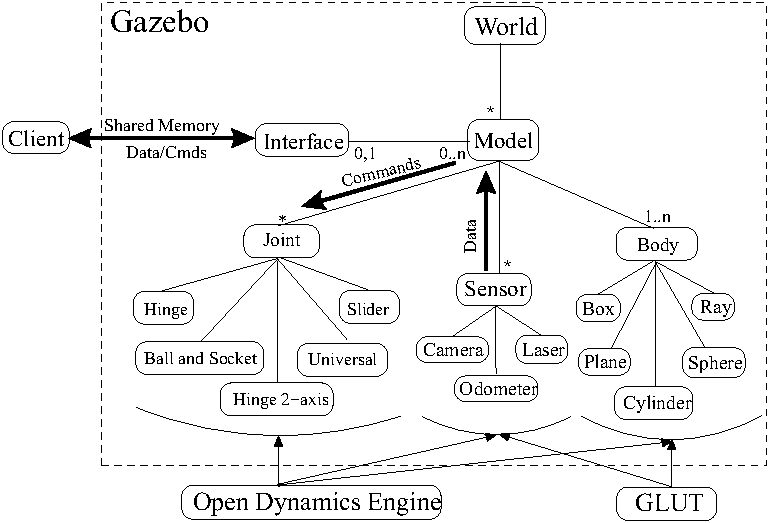
\includegraphics[height=10cm]{kapitel2/gazebo}
  \caption[Architektur des Gazebo-Frameworks]{Architektur des Gazebo-Frameworks \autocite{Koenig-2004-394}}
  \label{Kap2:gazeboarchitektur}
\end{figure}

\subsubsection{Physik-Engine}

Als Physik-Engine wird standardmäßig die \ac{ODE} genutzt. Es sind auch weitere Physik-Engines möglich, da diese austauschbar sind. Dies liegt daran, dass sie nicht fest in der Softwarearchitektur verdrahtet sind. Alternativ zum Standard können demnach Bullet, Simbody oder DART genutzt werden.
    
\subsubsection{Visualisierung}

Für die reine Visualisierung nutzt Gazebo standardmäßig OpenGL sowie GLUT (OpenGL Utility Toolkit). OpenGL ist plattformunabhängig, hochskalierbar, stabil und wird stetig weiterentwickelt. Außerdem sind viele Funktionalitäten in OpenGL auf Hardware-Ebene in der Grafikkarte entwickelt, so dass die CPU entlastet ist und andere Aufgaben schneller leisten kann.}

\subsubsection{Welt}

Die Gazebo-Welt ist eine Sammlung aus verschiedenen Komponenten:
\begin{itemize}
  \item \emph{Modelle}: Modelle sind Objekte mit einer physikalischen Definition.
  \item \emph{Körper}: Körper sind die grundlegenden geometrischen Bauteile beispielsweise des Roboters.
  \item \emph{Gelenke}: Gelenke verbinden die Körper miteinander und formen damit die möglichen kinematischen Bewegungen.
  \item \emph{Sensoren}: Ein Sensor in Gazebo ist ein abstraktes Gerät ohne physikalische Definition. Gazebo bietet aktuell einen Odometriesensor, einen Nähesensor sowie eine Kamera an.
\end{itemize}
  
\subsubsection{Erstellung von Modellen}

Aktuell müssen Modelle per Hand erstellt werden. Dies erfolgt in der Regel über das sdf-Format. Kommt \ac{ROS} zum Einsatz, kann mittels der Node urdf\_spawner auch das urdf-Format verwendet werden.}
  
Abschließend ist noch wichtig, dass Gazebo durch Plugins erweiterbar ist und eine umfangreiche Schnittstelle bietet, die in einem \ac{ROS}-Node mit C++ oder Python aufgerufen werden kann. Des Weiteren lässt Gazebo auch ein Rendering der Simulation auf einem Remote-Server zu, so dass verteilte Anwendungen möglich werden. Dies ist in vielen Fällen aufgrund begrenzter Rechenleistung von Vorteil. 

\subsection{Open Inventor}

TODO START

Ich denke, dass hier auch der Open Inventor hinein sollte. Stammt aus den 90ern von SGI. Dateiendung .iv Das wurde nach VRML weiterentwickelt und daraus ging schließlich X3D hervor. Entstanden sind daraus auch Szenengraphensysteme, etwa Open Scene Graph. 
Den Open Inventor gibt es heute noch. Der wird beispielsweise zur medizinischen Visualisierung benutzt (ggf. Zitat von Bernhard Preim, ich frage dazu auch gern bei Barbara Waldkirch oder Sandy Engelhardt nach. Bernhard kenne ich übrigens auch persönlich ...)
Eine Alternativ-Implementierung ist Coin3D, verwendet beispielsweise bei OpenRave. Dazu gibt es eine Diss von Rosen Diankov, Aus der ecke kommt auch IKfast. Bitte nachschauen, von wem IKfast tatsächlich ist.

TODO END

\section{Robotermodelle}

Der folgende Abschnitt gibt einen Überblick über die Verwendung von Robotermodellen in \ac{ROS} und Gazebo.

Robotermodelle können in \ac{ROS} in einem \ac{URDF} angegeben werden. Dieses Format beinhaltet jedes Segment und jedes Gelenk sowie deren Zusammenspiel. Dabei wird für jedes Segment die Visualisierung, der Massenschwerpunkt und die Trägheitsmomente sowie ein Kollissionsmodell angegeben. Die Gelenke beinhalten den Verweis auf das Eltern- und auf das Kindelement sowie einen Arbeitsbereich.

\begin{figure}[b!]
  \centering
  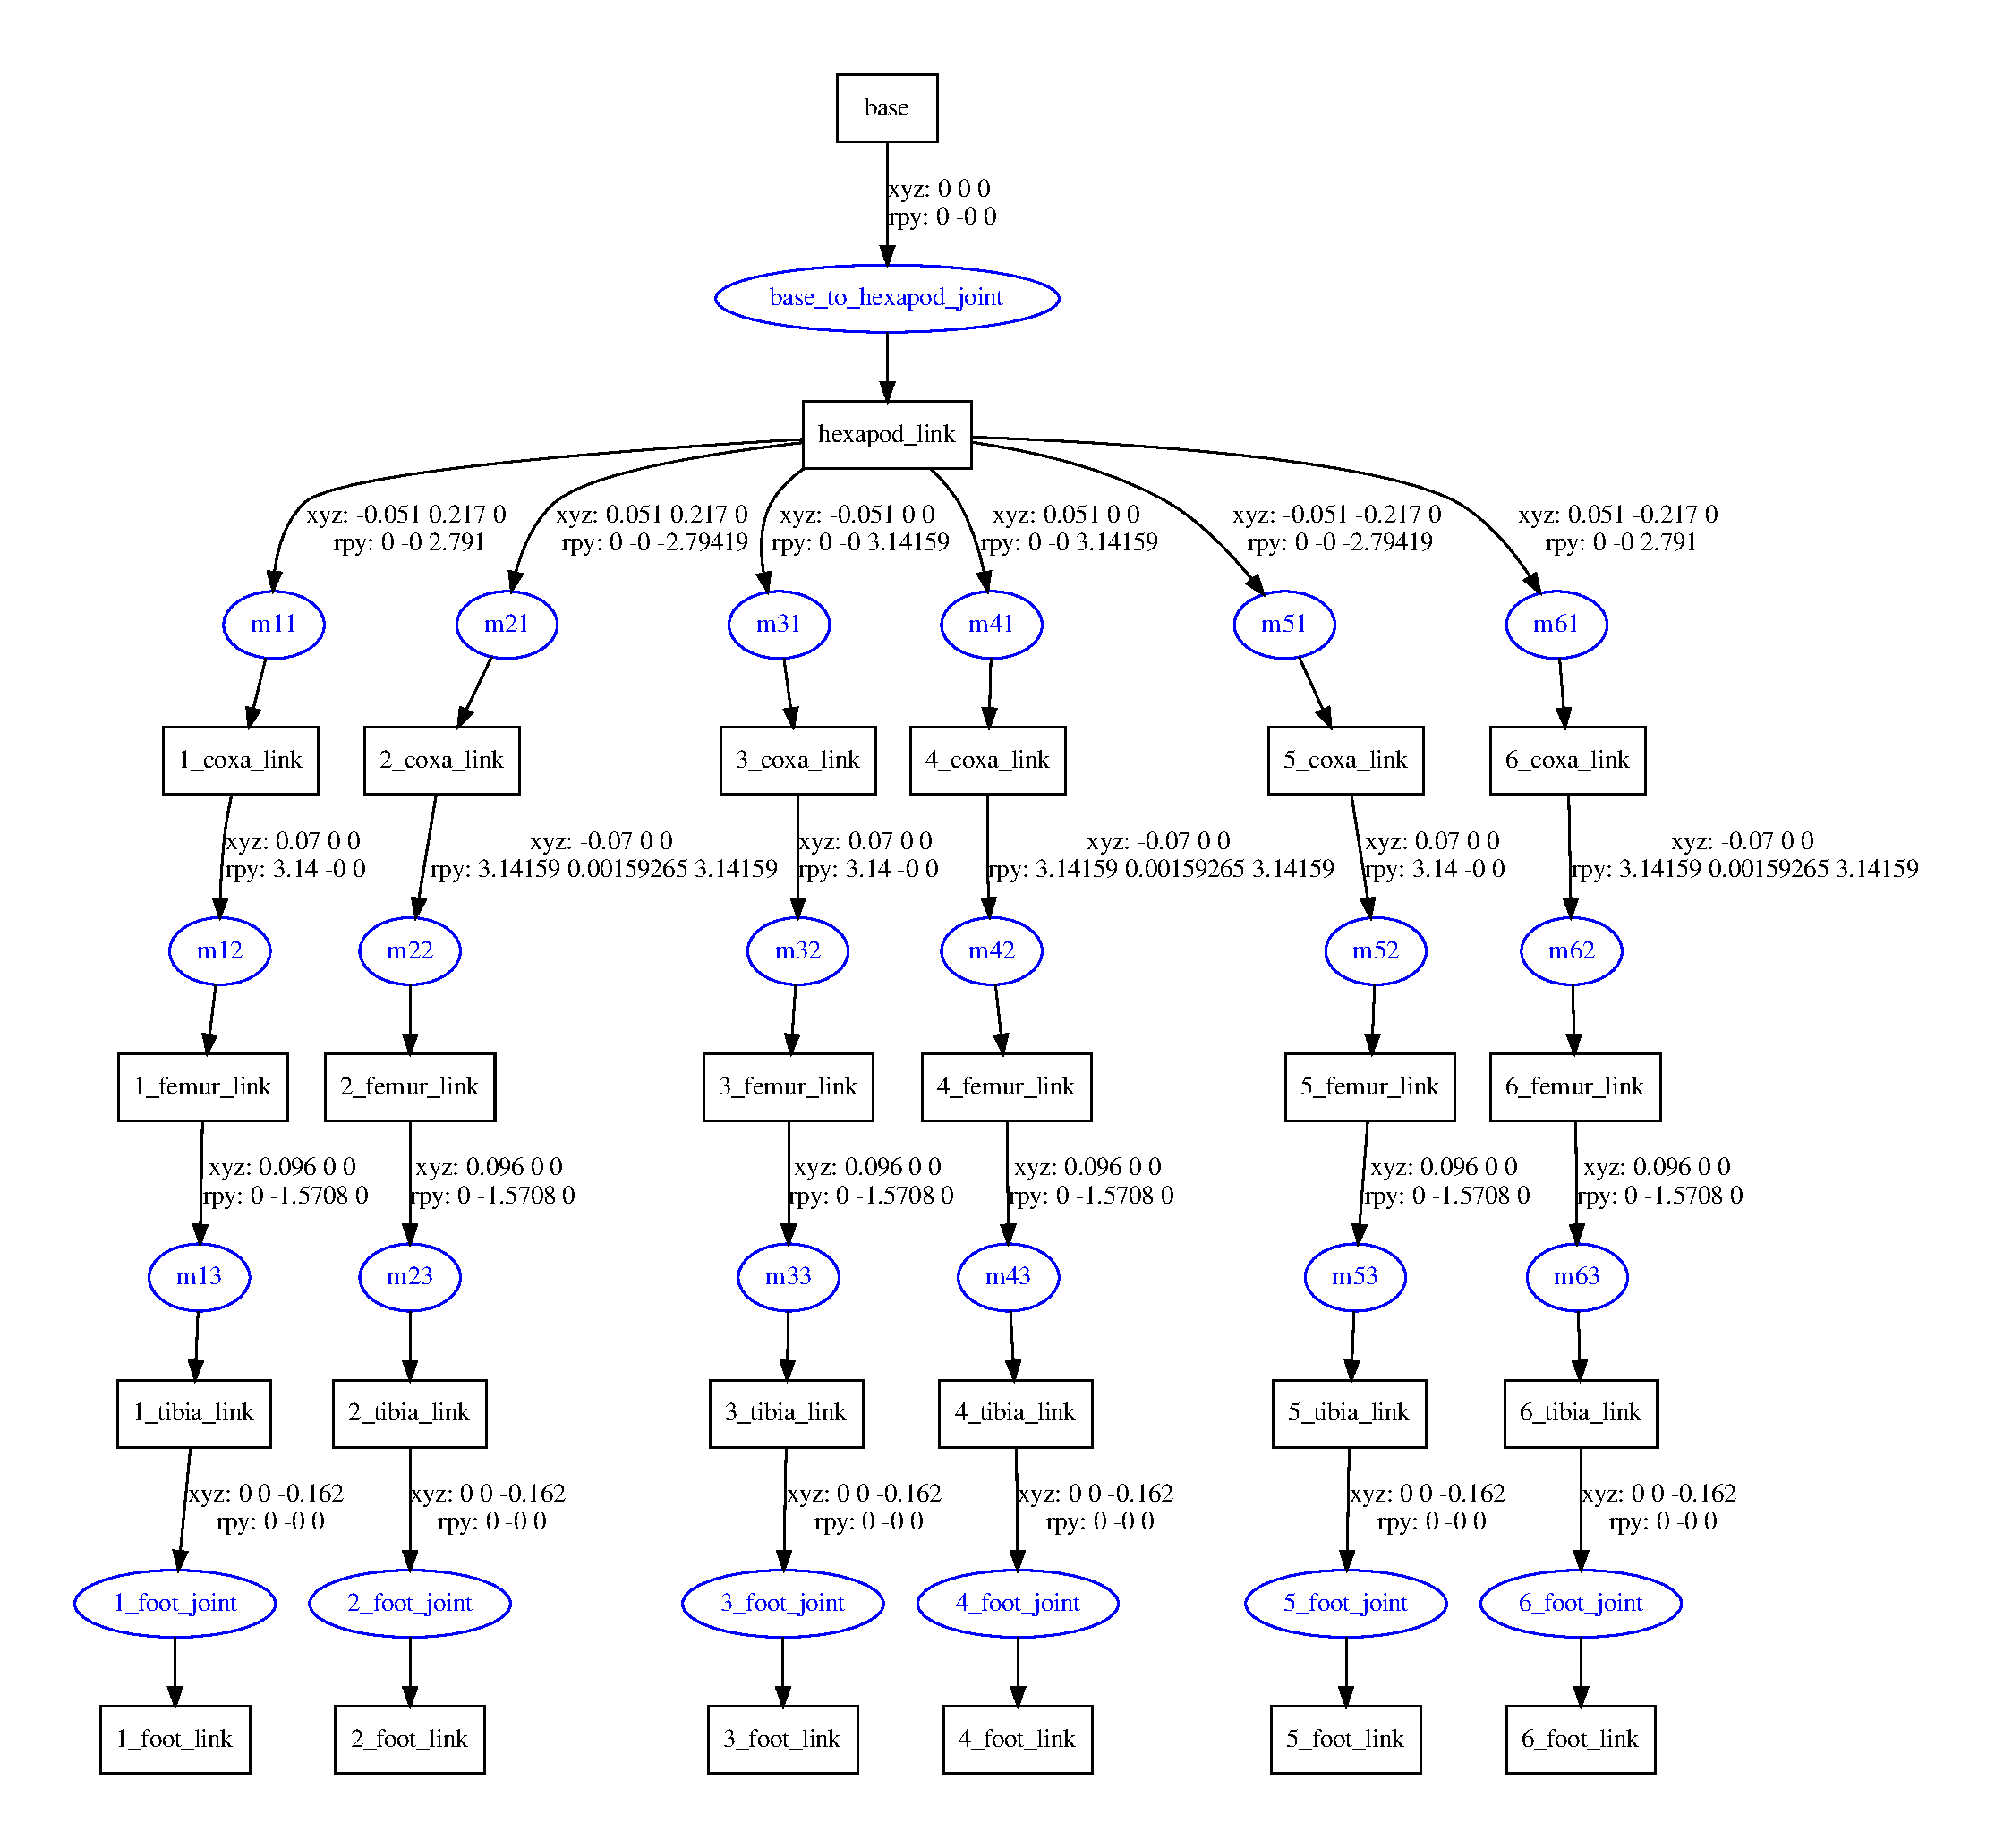
\includegraphics[height=8cm]{kapitel2/urdtographizakrobat}
  \caption{Darstellung des Transformationsbaums des Akrobats}
  \label{Kap2:urdtographizakrobat}
\end{figure}

Eine Möglichkeit das \ac{URDF}-Format zu verbessern bieten \ac{Xacro}. \ac{Xacro} zielt vor allem darauf ab das Format lesbarer und kürzer zu gestalten. Beispielsweise lassen sich über den \emph{include}-Befehl Dateien einbinden, was in \ac{URDF} nicht möglich ist. Über Tools wie den rviz, können Robotermodelle visualisiert werden. Mittels des Kommandozeilen-Tools urdf\_to\_graphiz lässt sich der Transformationsbaum eines Robotermodells visualisieren. Dies wird in \autoref{Kap2:urdtographizakrobat} am Beispiel des Akrobat dargestellt.

Nun wird auf die drei wesentlichen Modelle des \ac{URDF}-Formats eingegangen: Das Visualisierungmodell, das Kollisionsmodell und das Modell für Massenschwerpunkte und Trägheitsmomente.

\subsection{Aufsetzen der Visualisierung}

Beim Visualisierungsmodell gibt es zwei Möglichkeiten der Angabe eines Segments.
\begin{itemize}
\item Als \ac{STL}-Datei
\item Als geometrisches Objekt (z.B. ein Zylinder oder ein Quader)
\end{itemize}

Gerade bei Robotern wie dem Akrobat oder dem Lauron eignet sich die Verwendung einer \ac{STL}-Datei, da dort alle Details vorhanden sind und der Roboter real aussieht, während bei einem geometrischen Objekt keine Details sondern nur der grundlegende Aufbau erkennbar ist.

\subsection{Aufsetzen des Kollisionsmodells}

Auch das Kollssionsmodell kann entweder als \ac{STL}-Datei oder als geometrisches Objekt angegeben werden. Da die \ac{STL}-Dateien viel detaillierter sind, wird daher zwar mehr Rechenleistung benötigt, aber auch die physikalischen Bewegungen sehen damit realer aus. Eine Möglichkeit wäre es die 3D-Modelle mittels MeshLab \autocite{LocalChapterEvents:ItalChap:ItalianChapConf2008:129-136} runterzurechnen, so dass sie später besser von Gazebo verarbeitet werden können, da sie optimiert sind.

\subsection{Aufsetzen der Massenschwerpunkte und der Trägheitsmomente}

\begin{figure}[t!]
 \centering
 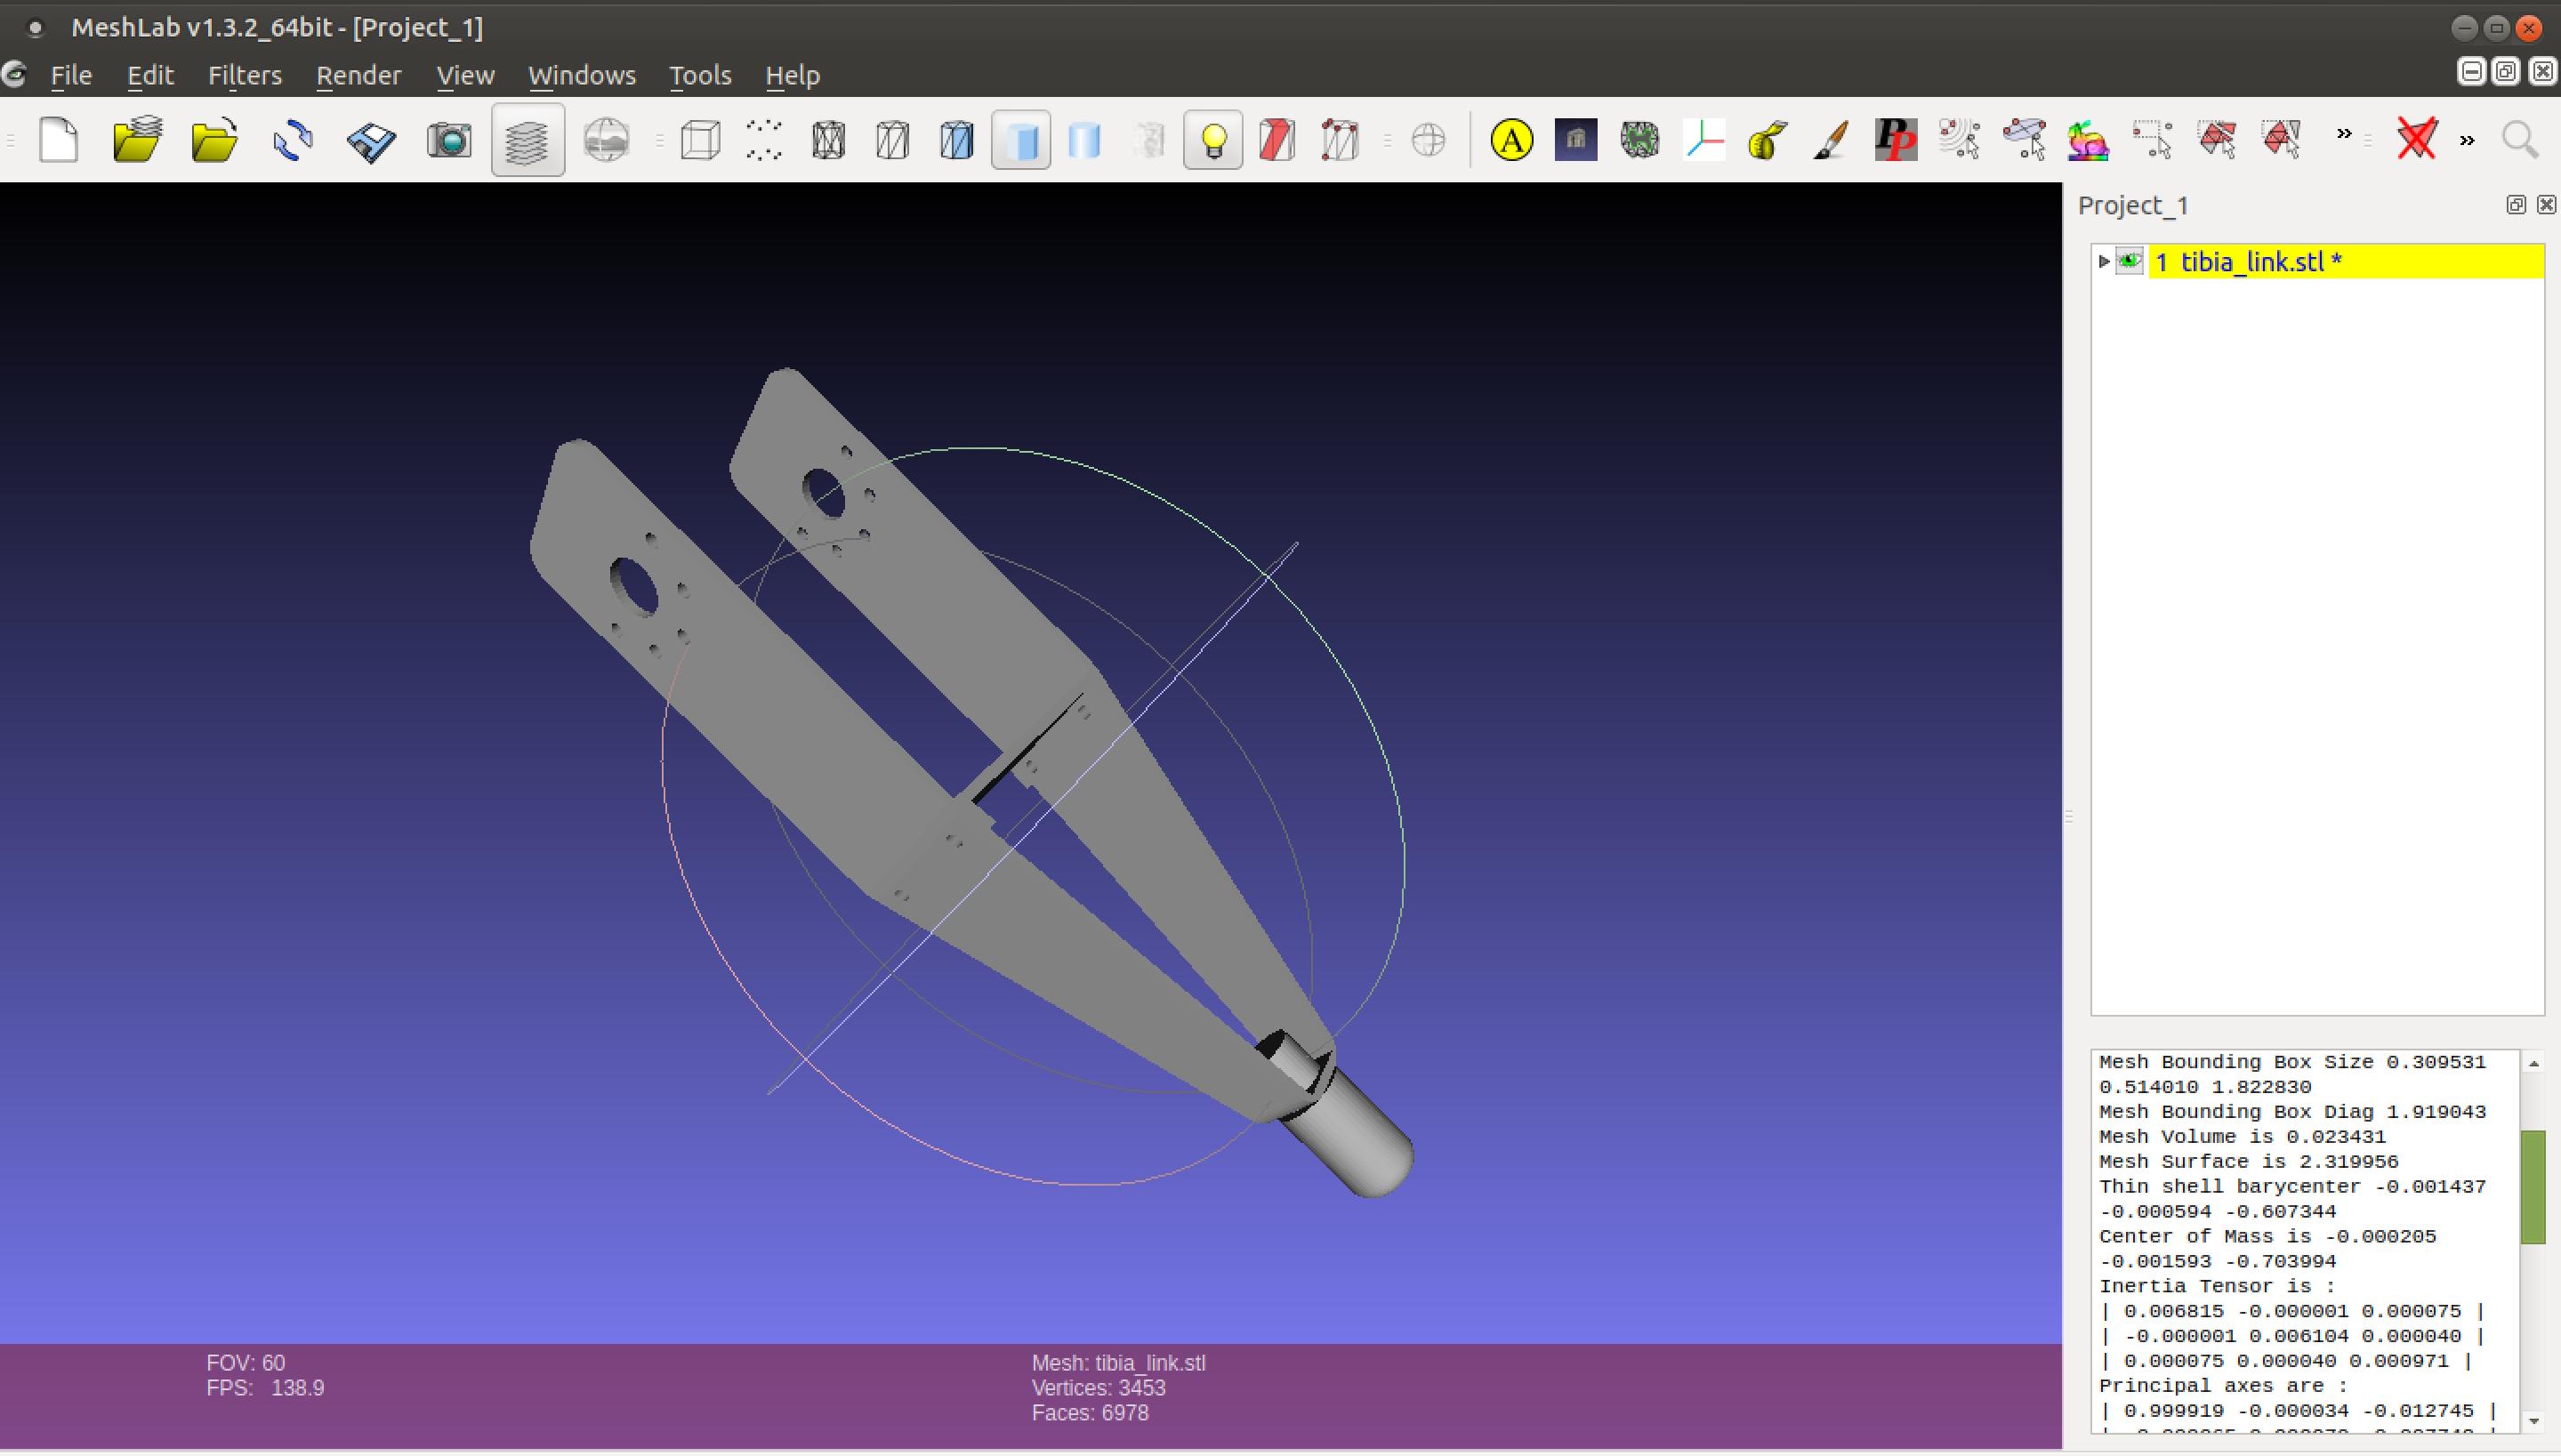
\includegraphics[height=8cm]{kapitel2/meshlab-inertia}
 \caption{Auslesen der Trägheitsmomente mit MeshLab}
 \label{Kap2:MeshLabInertia}
\end{figure}

Ebenfalls muss die Massenträgheit für jedes Körperteil einzeln definiert werden. Dabei wird eine Masse sowie das Trägheitsmoment angegeben. Die Masse lässt sich durch Wiegen der einzelnen Körperteile herausfinden. Um das Trägheitsmoment für das jeweilige Körperteil herauszufinden, bietet Gazebo die Möglichkeit die Werte über MeshLab auszulesen und umzuwandeln \autocite{gazebo-inertial}. \autoref{Kap2:MeshLabInertia} zeigt die Extraktion der Trägheitsmomente aus MeshLab. Da MeshLab das Ergebnis rundet, muss das Körperteil um einen Faktor $s$ skaliert werden, um eine höhere Genauigkeit zu erreichen. Dazu eignet sich ein Faktor von 10 oder 100. Erst dann kann die Berechnung über die berechnete Masse $m$ und dem berechneten Volumen $V$ sowie die Rückskalierung über den Faktor $s$ in \autoref{ml1} mit dem Ergebnis aus MeshLab $Ergebnis_{vorher}$ ausgeführt werden.

\begin{equation}
 Ergebnis_{nachher} = \frac{Ergebnis_{vorher} \cdot m \cdot V}{s}
\label{ml1}
\end{equation}

Zum Abschluss können die berechneten Trägheitsmomente aus dem $Ergebnis_{nachher}$ in die \ac{URDF}-Datei eingetragen werden.
\chapter{Verwandte Arbeiten}
\label{kap3}

Dieses Kapitel stellt weitere Arbeiten dar, die sich mit dem Thema der Laufplanung von sechsbeinigen Laufrobotern mittels Random Sampling auseinandergesetzt haben.

\section{André Herms}

Andrè Herms \autocite{herms2004} vergleicht zunächst die folgenden Algorithmen zur Laufplanung:
\begin{itemize}
  \item Random Sampling
  \item Greedy Verfahren
  \item Branch and Bound
  \item Lokale Suche
  \item Tabu-Suche
  \item Simulated Annealing
  \item Genetische Algorithmen
\end{itemize}

Dabei nutzt Herms die folgenden Kriterien:
\begin{itemize}
  \item Parallelisierbarkeit
  \item Speicherbedarf
  \item Anytime-Fähigkeit
  \item Allgemeine Anwendbarkeit
\end{itemize}

Es stellt sich heraus, dass nur die Algorithmen \emph{Random Sampling}, \emph{Lokale Suche} und \emph{Simulated Annealing} alle Kriterien mindestens erfüllen. Nach der Implementierung und erster Tests stellt sich heraus, dass das Random Sampling die Kriterien am besten erfüllt, da die Lokale Suche sowie das Simulated Annealing die Lösungen zu langsam erstellen. \autoref{Kap3:BewertungRandomSampling} bewertet das Random Sampling anhand der genannten Kriterien. Auch hier wird nochmals deutlich, dass das Random Sampling positiv abschneidet.

\begin{table}[!t]
  \caption{Bewertung des Random Samplings}
  \label{Kap3:BewertungRandomSampling}
  \renewcommand{\arraystretch}{1.2}
  \centering
  \sffamily
  \begin{footnotesize}
    \begin{tabularx}{0.9\textwidth}{l X}
      \toprule
      \textbf{Kriterium} & \textbf{Erfüllung}\\
      \midrule
      \emph{Parallelisierbarkeit} & Lösungen können ohne großen Aufwand unabhängig voneinander generiert werden. Am Ende müssen diese nur noch synchronisiert werden, so dass die Lösung mit der besten Bewertung übernommen wird.\\
      \addlinespace
      \emph{Speicherbedarf} & Der Algorithmus benötigt kaum Speicher, da immer nur eine Lösung generiert wird und diese die vorherige beste Lösung überschreibt.\\
      \addlinespace
      \emph{Anytime} & Das Kriterium ist erfüllt, sobald eine Lösung generiert ist. Allerdings kann es passieren, dass in einer bestimmten Zeit noch keine gute Lösung vorhanden ist.\\
      \addlinespace
      \emph{Anwendbarkeit} & Der Algorithmus lässt sich auf jedes Problem der Laufplanung anwenden. Die Qualität hängt allerdings vom Anteil guter Lösungen, die im Lösungsraum vorhanden sind. Außerdem spielt die konkrete Implementierung des Algorithmus eine große Rolle. Insgesamt gilt, dass je länger der Algorithmus läuft, desto besser sind potentiell die Lösungen.\\
      \bottomrule
    \end{tabularx}
  \end{footnotesize}
  \rmfamily
\end{table}

Daher entscheidet die Arbeit von André Herms, dass das Random Sampling für den Laufplaner genutzt werden soll, da es zwischen allen Algorithmen am besten abschneidet.

Der von André Herms daraufhin entwickelte Laufplaner für den \emph{Lauron III} basiert auf der 3D-Bibliothek OpenInventor \autocite{inventor}. Dieses Toolkit basiert wiederum auf OpenGL und ist in C++ implementiert. Des Weiteren ist es objektorientiert implementiert. Auf Grund dieser Tatsache existieren Klassen bzw. Objekte, die nun beschrieben werden:
\begin{itemize}
  \item \emph{World}: speichert die Objekte der Sicht auf die Landschaft und den Roboter. 
  \item \emph{Terrain}: enthält die Informationen über die Höhenkarte.
  \item \emph{Eyes}: stellt die Sicht auf die Landschaft dar.
  \item \emph{Robot}: ist verantwortlich für die Robotersteuerung und definiert außerdem die inneren Objekte \emph{Head} und \emph{Leg}.
\end{itemize}  
  
\begin{figure}[t!]
  \centering
  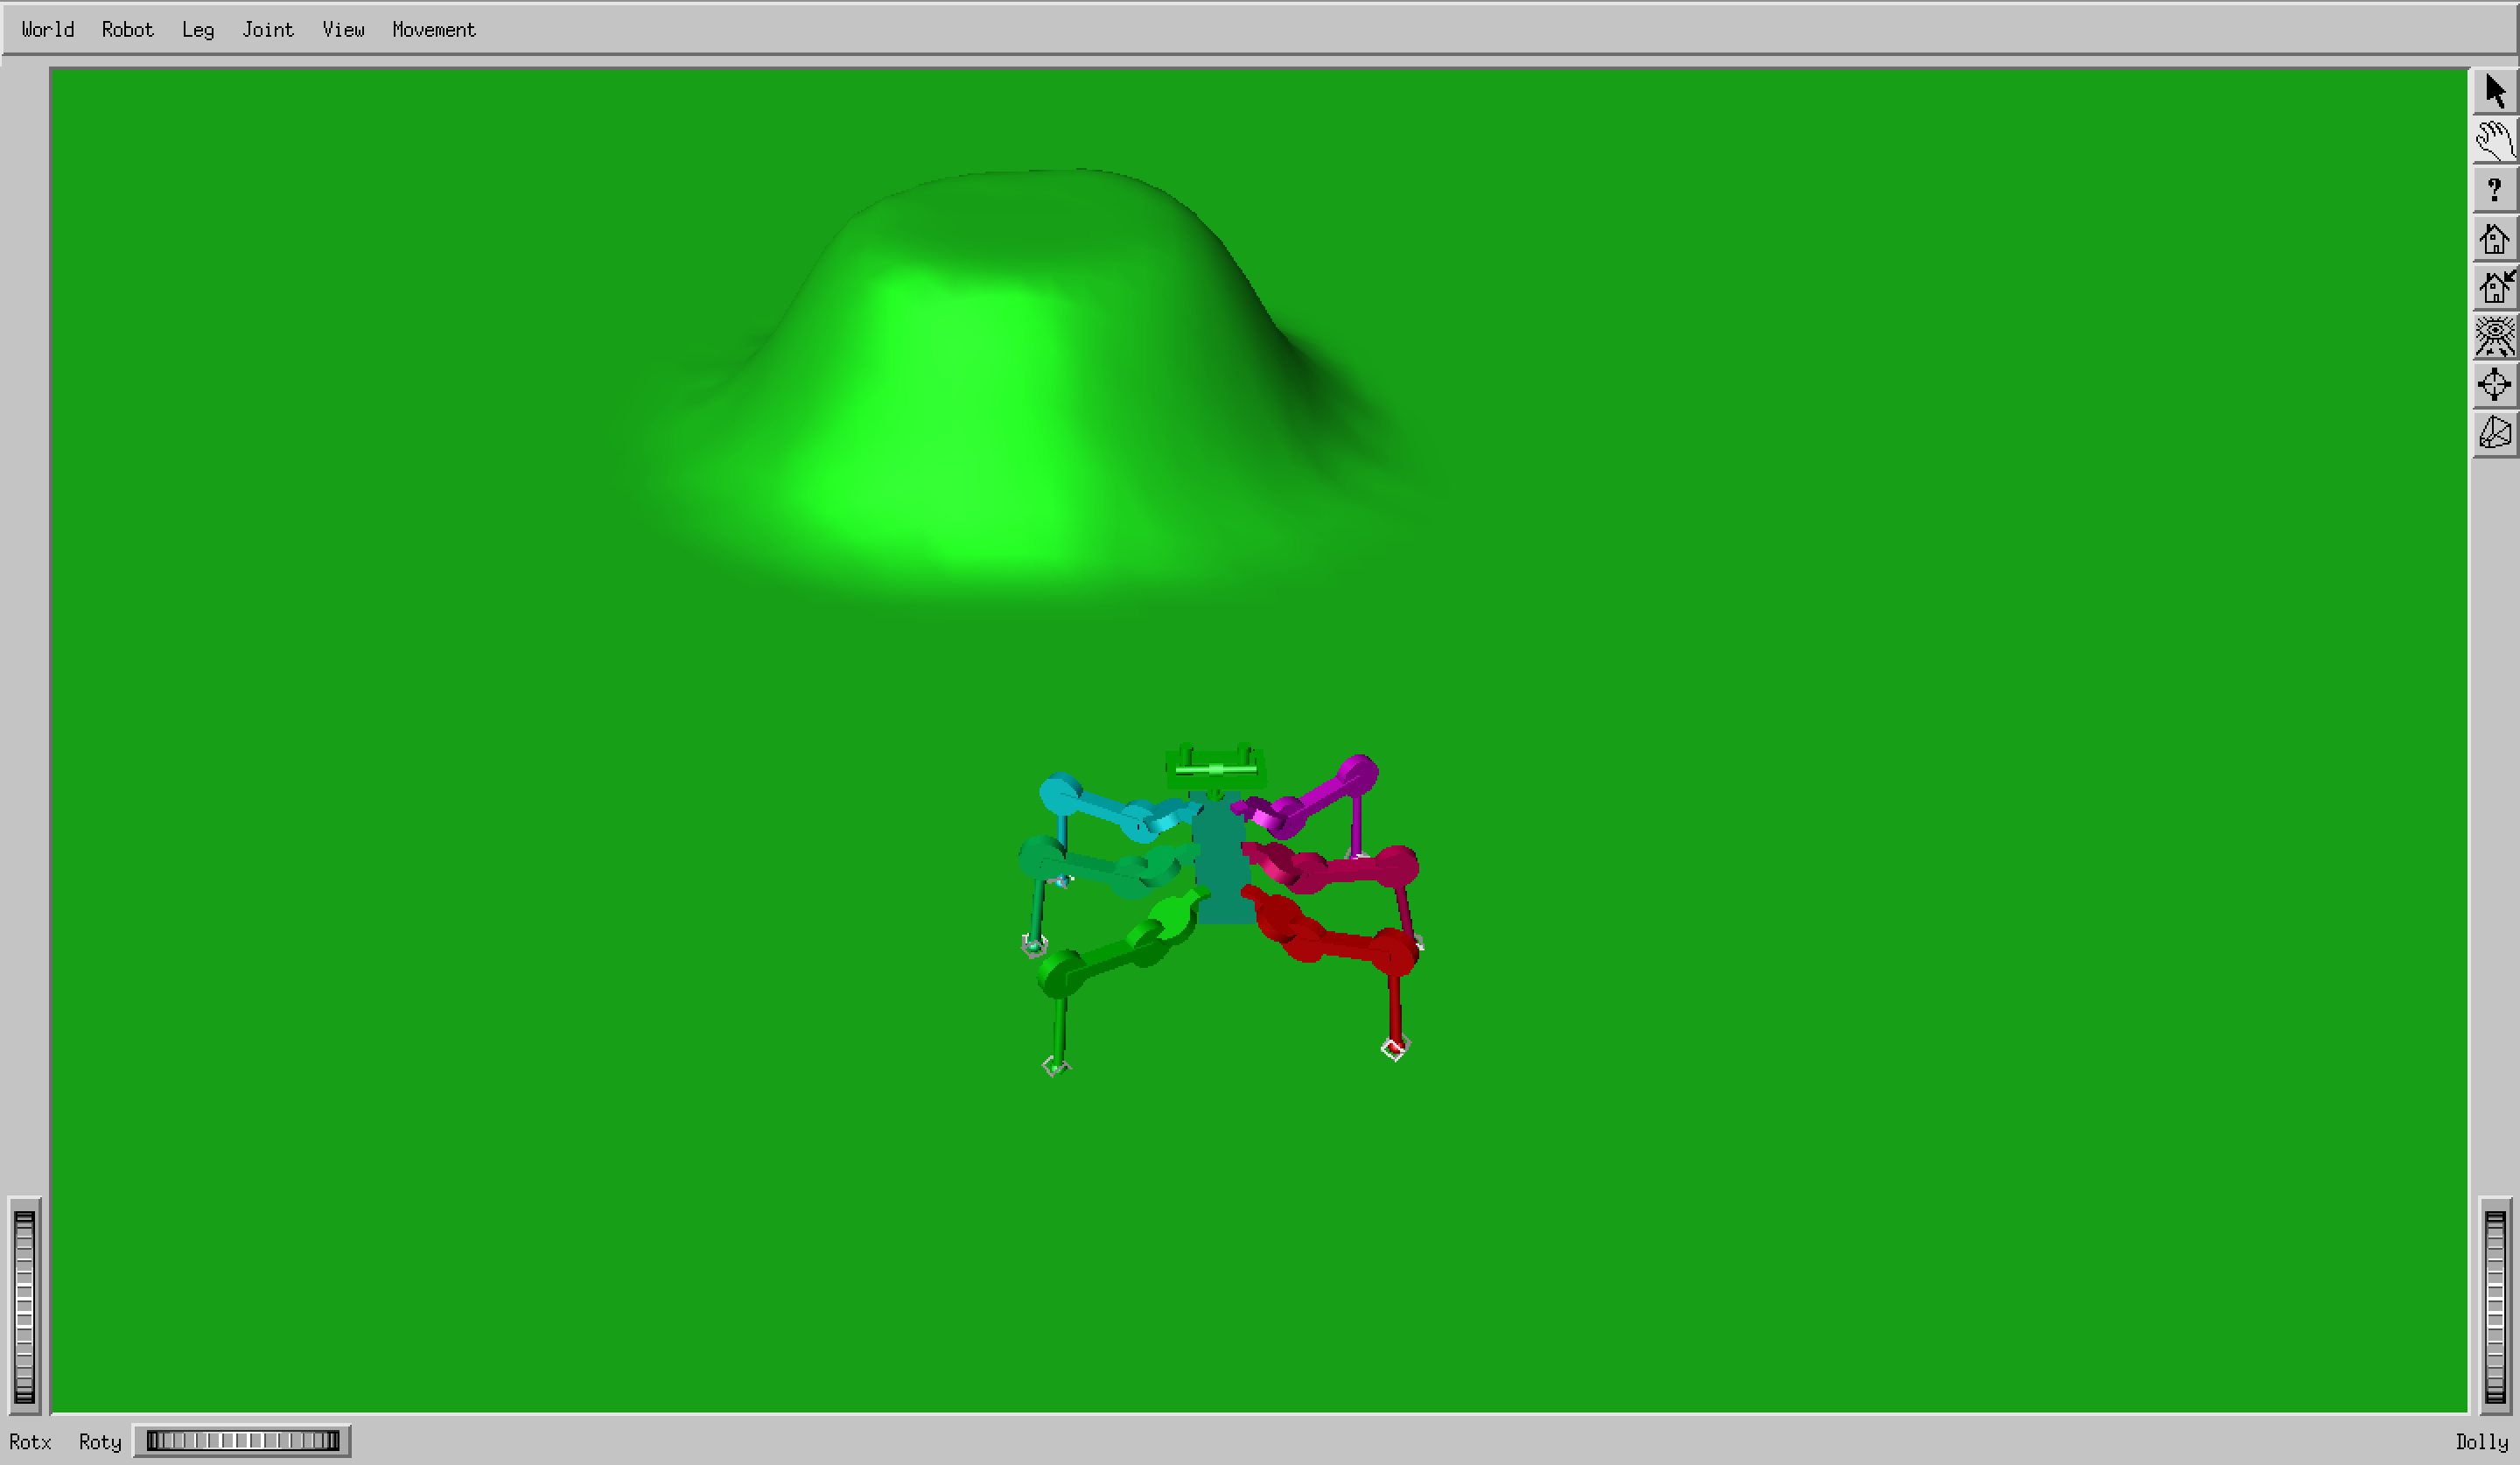
\includegraphics[height=8cm]{kapitel3/openinventor-lauron}
  \caption{Screenshot aus der OpenInventor-Umgebung}
  \label{Kap4:OpenInventorLauron}
\end{figure}

Für jedes dieser Darstellungsobjekt in OpenInventor wird ein \emph{SoSeperator} benötigt. Da der Name dieses Objekts einzigartig sein muss, sind die Objekte auch nur einmalig nutzbar. Dies erschwert die Aufgabe, später einmal mehrere Roboter gleichzeitig in der Simulation zu testen. Code-technisch sollte das dem Design-Pattern \emph{Singleton} folgen. Der Laufplaner sichert diese allerdings nicht derart ab.

Des Weiteren stellt das Terrain-Objekt die Höhenkarte der Landschaft in OpenInventor zur Verfügung. Dies entspricht nicht dem, was dem Roboter tatsächlich an Kartenmaterial zur Verfügung hat.

Eine Konfigurationsdatei existiert bereits in dieser Umgebung, die es ermöglichen soll, auch andere Robotermodelle zu testen. Diese wird für den Laufalgorithmus allerdings nicht genutzt, da dort Roboterangaben direkt im Quelltext definiert sind.

Weiterhin wird die aktuelle Fußkonfiguration sowie die Fußposition getrennt voneinander gespeichert. Die Fußkonfiguration ist in einer Bitlogik gespeichert. Dies ist sehr nützlich um Speicherplatz zu sparen, macht auf der anderen Seite das Finden von Fehlern allerdings schwieriger.

\section{Uli Ruffler}

Uli Ruffler \autocite{ruffler2006} hat den Laufplaner auf eine inkrementelle Arbeitsweise angepasst. Des Weiteren hat er die Basis für die Stereobildverarbeitung gelegt. Der Laufplaner kann nun während des Laufens neue Lösungen generieren, allerdings werden diese Lösungen noch nicht verwendet.
\chapter{Konzeption der Lösung}
\label{kap4}

Dieses Kapitel nutzt die in \autoref{kap3} dargestellten verwandten Arbeiten, um ein Konzept für die Portierung des Laufplaners für den Akrobat in \ac{ROS} und Gazebo formal darzustellen. Als Basis dafür werden die Arbeiten von André Herms \autocite{herms2004} und Uli Ruffler \autocite{ruffler2006} herangezogen. Für die Darstellung einer Lösung sind zwei Aspekte von Bedeutung. Dies ist zum einen die Simulationsumgebung. Zum anderen ist dies der Laufplanungsalgorithmus. Beide Aspekte können getrennt voneinander betrachtet werden.

\section{Simulationsumgebung} 

Damit die Simulationsumgebung möglichst nahe an der Software des Laufroboters Akrobat sein soll, soll in beiden Fällen das \ac{ROS} genutzt werden. Um die reale Umgebung zu simulieren, benötigt die Lösung eine Physik-Engine, die bei André Herms \autocite{herms2004} Simulationsumgebung nur rudimentär vorhanden ist. Bei der Nutzung von Gazebo wird standardmäßig die \acf{ODE} mitgeliefert, welche auch hierbei zum Einsatz kommen soll.

Zusätzlich soll es möglich sein, verschiedene Umgebungen laden zu können, damit die Flexibilität beim Testen der Laufalgorithmen erhalten bleibt. Dies ist mit Hilfe von verschiedenen Gazebo-Welten zu lösen. Im ersten Schritt soll dazu eine leere Welt genutzt werden.

Um außerdem ein möglichst reales Szenario zu simulieren, muss ein präzises Robotermodell im Format \ac{URDF} für das \ac{ROS} und Gazebo zum Einsatz kommen, welches das Aussehen, das Kollissionsmodell sowie die Massenträgheit genau beschreibt. Der bestehende Laufplaner besitzt aktuell noch das Modell des \emph{Lauron III}, welches in der neuen Lösung keine Anwendung mehr findet.

Des Weiteren sollen die Gelenkbewegungen nicht mehr über OpenInventor \autocite{inventor} ausgeführt werden. Dazu soll ein \ac{ROS}-spezifisches Paket mit dem Namen \emph{ros\_control} verwendet werden. Durch dieses werden Motoren an den Gelenken simuliert, welche über \ac{ROS}-Topics angesteuert werden können.

\section{Laufplanung}

Da der Laufplaner und die Simulation voneinander getrennt sein sollen, damit das System flexibel für den Austausch von Komponenten bleibt, benötigt der Laufplaner ebenso wie bei André Herms und Uli Ruffler eine xml-Schnittstelle, welche Bewegungen repräsentiert. Die hier dargestellte Schnittstelle soll eine Abwandlung der vorherigen Schnittstellen sein, da diese nicht die Dauer von Bewegungen speichert, sondern lediglich für jeden Schritt die Fußpositionen relativ zur definierten Ausgangsposition. Wie im Vorgängermodell sollen Bewegungen generiert und auch eingelesen werden können.

Der vorherige Laufplaner hat kinematische Berechnungen manuell in OpenInventor durchgeführt. Das neue System soll das \ac{ROS}-Framework \textsc{tf} verwenden, um möglichst einfach Koordinatentransformationen sowie die direkte und inverse Kinematik zu berechnen. Auch für weitere geometrische Berechnungen soll ausschließlich das \textsc{tf}-Framework zum Einsatz kommen.

Des Weiteren muss der Algorithmus auf den Laufroboter Akrobat angepasst werden, da der vorherige Algorithmus auf dem \emph{Lauron III} basiert und die Maße andere sind.
\chapter{Implementierung in ROS und Gazebo}
\label{kap5}

Dieses Kapitel stellt eine Implementierung für das in \autoref{kap4} dargestellte Konzept der Entwicklung einer Simulationsumgebung und der Portierung des Algorithmus Random Sampling zur Laufplanung für den Akrobat dar.

\section{Vorgehensweise und Aufbau des Pakets}

Da eine komplette Kopie des vorherigen Algorithmus zur Laufplanung auf Grund verschiedener Umgebungen nicht möglich ist, ist die Vorgehensweise schrittweise wichtige Codestellen zu übertragen und zu testen. Dies hat den Vorteil, dass Funktionen unabhängig voneinander getestet werden können. Damit ergibt sich der folgende Gesamtablauf für die Portierung:
\begin{enumerate}
  \item Aufsetzen des \ac{ROS}-Pakets
  \item Aufsetzen des Pakets
  \begin{enumerate}
    \item Aufsetzen des Roboter-Modells
    \item Aufsetzen der Gelenkmotoren
  \end{enumerate}
  \item Aufsetzen der Fußsteuerung
  \item Testen der Fußsteuerung
  \item Portierung des Laufalgorithmus
\end{enumerate}

Während der Arbeit hat es sich als sinnvoll herausgestellt, die Portierung des Laufplaners erst zum Schluss zu beginnen und mit dem Aufsetzen der Simulation zu beginnen. Der Grund dafür ist, dass es damit während der Portierung möglich ist schon Artefakte in der Simulation zu testen. Damit lässt sich wesentlich besser einschätzen, ob das Übertragene auch funktioniert. Außerdem basiert der Laufplaner auf Funktionalitäten wie dem Roboter-Modell und der Definition der Gelenkmotoren. Mit dieser Vorgehensweise kann das Paket nun schrittweise implementiert werden.

\autoref{Kap4:ROSPackageFolderStructure} definiert die Ordnerstruktur des \ac{ROS}-Pakets. Die Ordnerstruktur ist typisch für \ac{ROS}-Pakete und findet sich ähnlich in vielen weiteren Paketen der \ac{ROS}-Community. Der Aufbau des Pakets ist an das Akrobat-Paket \autocite{akrobat} sowie das Hopper-Paket \autocite{hopper} angelehnt. Beide Pakete nutzen wichtige Konzepte für das Robotermodelle und die Gelenksteuerung, die auch für dieses Projekt wichtig sind.

\begin{figure}[p!]
\dirtree{%
.1 hexapod.
.2 config.
.3 config.rviz.
.3 hexapod.yaml.
.2 urdf.
.3 hexapod.xacro.
.3 leg-1.xacro.
.3 leg-2.xacro.
.3 leg-3.xacro.
.3 leg-4.xacro.
.3 leg-5.xacro.
.3 leg-6.xacro.
.2 launch.
.3 rviz.launch.
.3 gazebo.launch.
.3 model.launch.
.3 akrobat\_walk.launch.
.3 control.launch.
.2 include.
.3 akrobat.
.4 akrobat\_init.h.
.4 JointStateToGazebo.h.
.4 ControlRandomSampling.h.
.4 JointStateToDynamixel.h.
.4 FootConfiguration.h.
.4 Akrobat.h.
.3 pugixml.
.2 worlds.
.3 default.world.
.2 stl.
.3 hexapod\_link.stl.
.3 coxa\_r\_link.stl.
.3 coxa\_l\_link.stl.
.3 femur\_link.stl.
.3 tibia\_link.stl.
.2 src.
.3 akrobat.
.4 akrobat\_main.cpp.
.4 JointStateToGazebo.cpp.
.4 FootConfiguration.cpp.
.4 JointStateToDynamixel.cpp.
.4 Akrobat.cpp.
.4 ControlRandomSampling.cpp.
.3 pugixml.
}
\caption{Dateibaum des ROS-Pakets}
\label{Kap4:ROSPackageFolderStructure}
\end{figure}

\section{Aufsetzen der Simulation}

Das erste Ziel ist es nun, den Akrobat in Gazebo anzuzeigen. Dazu muss das Robotermodell integriert werden, die Gelenkmotoren definiert werden und die Gazebo-Welt aufgesetzt werden.

\subsection{Aufsetzen des Robotermodells mittels \ac{URDF}}

Als erstes wird das Robotermodell in das neue \ac{ROS}-Paket integriert. Die vorliegende Roboterbeschreibung liegt im \ac{URDF}-Format vor. Des Weiteren existieren die 3D-Modelle im \emph{stl}-Format, welche im Robotermodell eingebunden sind. Damit das Robotermodell auch bei späteren Änderungen noch wartbar bleibt, wird die zusammenhängende Datei in das \ac{Xacro}-Format umgebaut, so dass nun eine Datei für die Robotermitte und eine Datei für jedes einzelne Bein existiert. Mit diesem Aufbau könnte das Robotermodell nun schon über ein Launch-File im 3D Visualisierungs-Tool "`rviz"' angezeigt werden. \autoref{Kap4:AkrobatRviz} zeigt stellt dies sowie die Koordinatensystemen des Roboters dar.

\begin{figure}[b!]
  \centering
  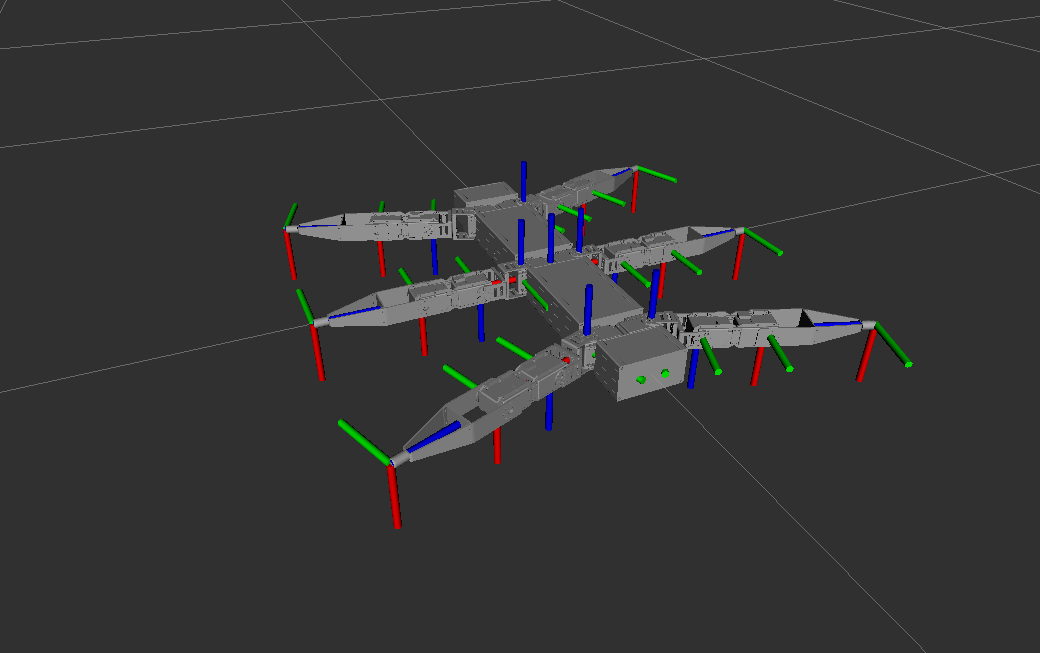
\includegraphics[height=8cm]{kapitel4/akrobat-rviz}
  \caption{Darstellung des Akrobats im rviz}
  \label{Kap4:AkrobatRviz}
\end{figure}

Für das spätere Hinzufügen des Akrobats in die \emph{Gazebo}-Simulation müssen neben der Visualisierung, die für den rviz ausreichend war, noch weitere Anpassungen am Roboter-Modell vorgenommen werden:
\begin{itemize}
  \item Aufsetzen des Kollisionsmodells durch das Attribut <collission>
  \item Aufsetzen der Massenschwerpunkte und der Trägheitsmomente durch das Attribut <inertia>
\end{itemize}

Danach ist das statische Modell fertig aufgesetzt. Nun müssen die Gelenkmotoren an den Gelenken definiert werden, damit diese von \ac{ROS} angesteuert werden können.

\subsection{Definition der Gelenkmotoren mittels ros\_control}

Das zuvor aufgesetzte Robotermodell könnte nun in Gazebo angezeigt werden. Allerdings ist dieses noch nicht durch Eingaben von außen beweglich, da keine Gelenkmotoren definiert sind. Diese werden in diesem Abschnitt behandelt.

Hierbei hat sich das Paket \emph{ros\_control} als geeignet herausgestellt. Für das Aufsetzen des Pakets wird eine Konfigurationsdatei für die Definition aller Controller benötigt. Außerdem muss im Robotermodell ein Gelenk auf einen Controller abgebildet werden, damit das Gelenk angesteuert werden kann. Außerdem müssen zwei wesentliche Plugins eingebunden und konfiguriert werden:
\begin{itemize}
  \item gazebo\_ros\_control
  \item p3d\_base\_controller
\end{itemize}

Abschließend muss die Konfigurationsdatei geladen und zwei \ac{ROS}-Nodes gestartet werden. Dies ist zum einen der \emph{robot\_state\_publisher}, der die publizierten Bewegungen an den Roboter weitergibt, sowie ein \emph{controller\_manager}, der letztendlich die einzelnen Gelenke in der Simulation bewegt. Hier lässt sich statt dem \emph{controller\_manager} auch direkt ein \emph{dynamixel\_manager} anbinden, so dass später leicht zwischen Simulation und dem realen Roboter gewechselt werden kann. Durch die Einbindung existieren nun zur Laufzeit einige wichtige \ac{ROS}-Topics, wie in \autoref{Kap4:RosControlTopics} zu sehen ist.

\begin{figure}[p!]
  \centering
  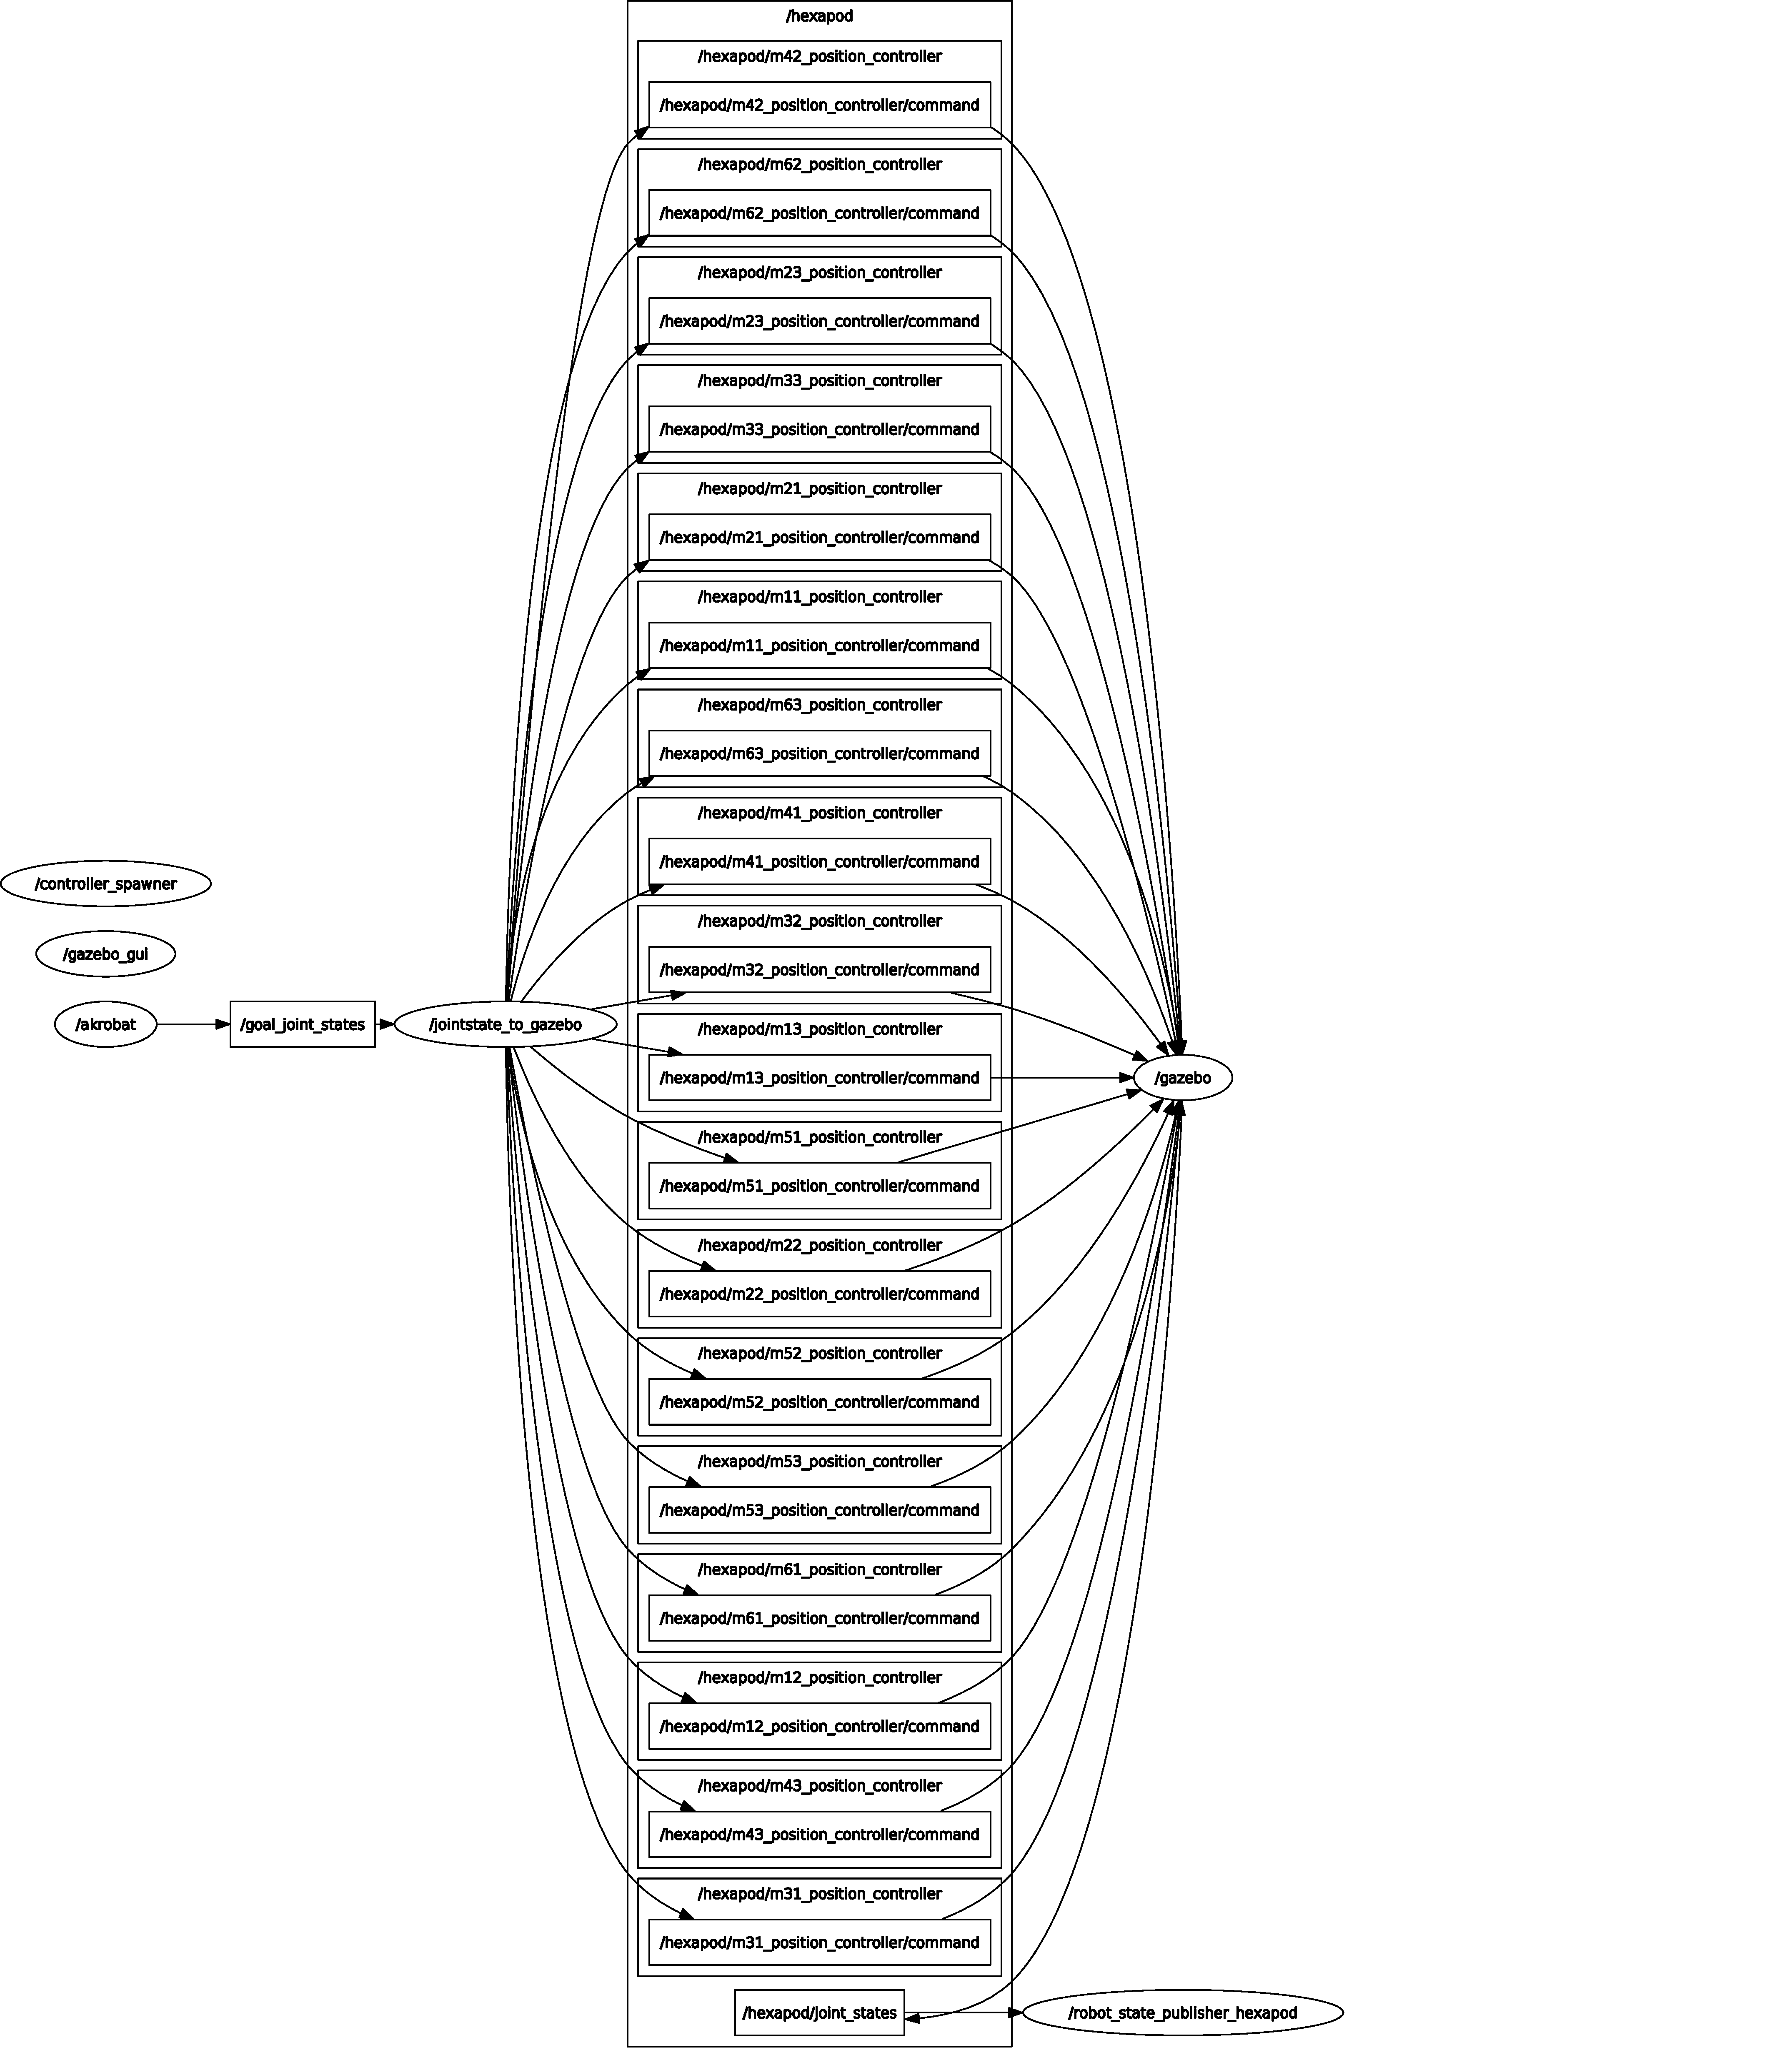
\includegraphics[height=23cm]{kapitel4/rosgraph}
  \caption{ROS-Topics der Simulation}
  \label{Kap4:RosControlTopics}
\end{figure}

\subsection{Aufsetzen der Umgebung mittels Gazebo}

Nun fehlt nur noch die Gazebo-Umgebung. Diese lässt sich mit einem von Gazebo bereitgestellten Launch-File starten. Es besteht die Möglichkeit Parameter mitzugeben. Die folgende Auflistung beschreibt einige wichtige Parameter:
\begin{itemize}
  \item \emph{world\_name}: Dateipfad zur gewünschten Welt
  \item \emph{debug}: Gibt Informationen zur Analyse während der Laufzeit aus
  \item \emph{gui}: Startet die grafische Oberfläche
  \item \emph{paused}: Pausiert die Simulation
\end{itemize}

Damit ist das Aufsetzen des Roboters sowie der Simulationsumgebung vollständig. Der Roboter wird nun in Gazebo angezeigt, wie in \autoref{kap4:gazeboflach} zu sehen ist.

\section{Aufsetzen der Ausgangsposition}

Der Roboter wird nun zwar im Gazebo angezeigt, allerdings liegt dieser nun flach auf dem Boden. Das Ziel ist es daher, die Fußsteuerung aufzusetzen, so dass der Roboter sich zu Beginn in seine Ausgangsstellung begibt. Von dort aus wartet der Roboter auf weitere Befehle für die Bewegung.

\begin{figure}[b!]
  \centering
  \begin{subfigure}[b]{.4\linewidth}
    \centering
    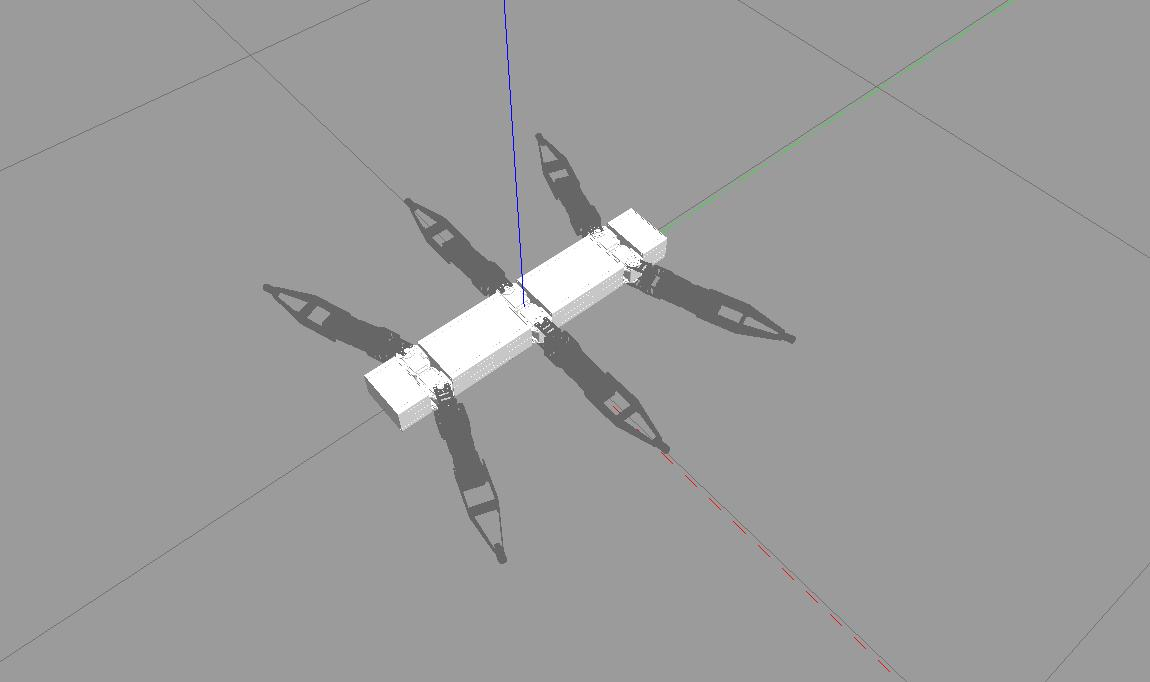
\includegraphics[width=6cm]{kapitel4/akrobat-flach}
    \subcaption{Vor Aufsetzen der Ausgangsposition}\label{kap4:gazeboflach}
  \end{subfigure}%
  \qquad
  \begin{subfigure}[b]{.4\linewidth}
    \centering
    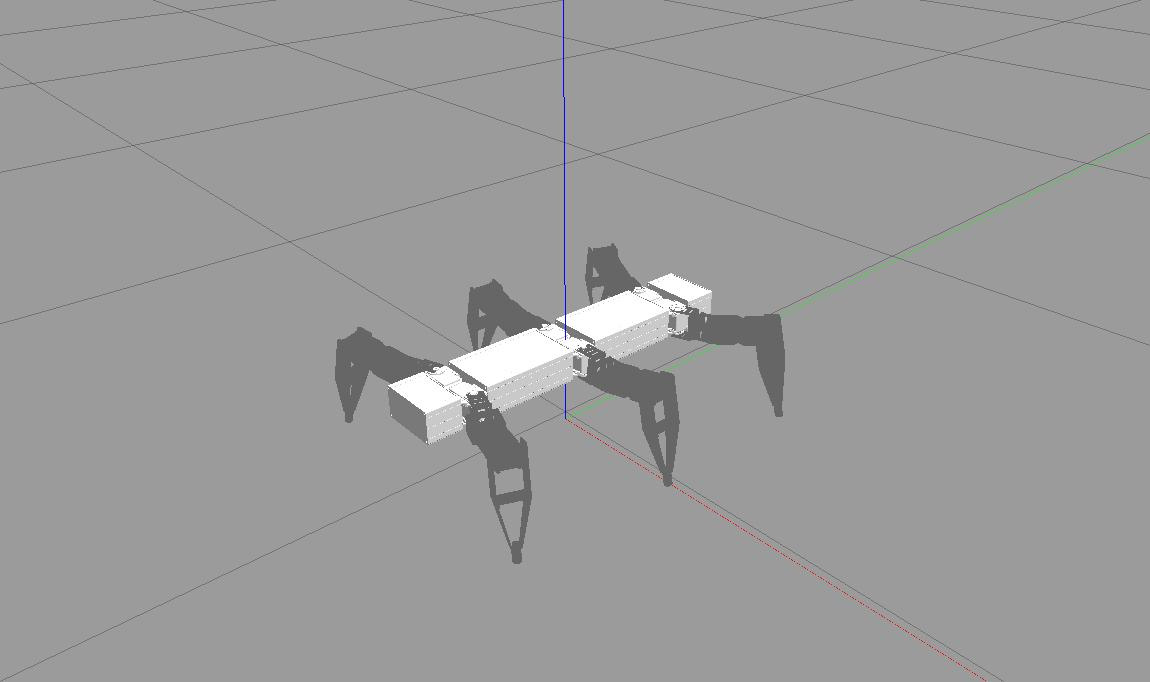
\includegraphics[width=6cm]{kapitel4/akrobat-oben}
    \subcaption{Nach Aufsetzen der Ausgangsposition}\label{kap4:gazebooben}
  \end{subfigure}\\
  \caption{Aufstehen des Akrobat in Gazebo}
  \label{kap4gazebo}
\end{figure}

Da \ac{ROS}-Nodes allgemein in einer Schleife laufen, wird der folgende Ablauf kontinuierlich ausgeführt. Der Ablauf sorgt wie in \autoref{kap4:gazebooben} zu sehen, dafür, dass der Roboter in den nächsten Durchläufen in der Ausgangsposition steht. Dies erfolgt in mehreren Schritten: 
\begin{enumerate}
  \item Zunächst wird über das \textsc{tf}-Framework} mit Hilfe von Transformationen und Rotationen die Ausgangsposition vom obersten Gelenk zum Endeffektor berechnet. Dies wird im weiteren Verlauf als Ausgangsposition definiert und eingelesene Bewegungen sind relativ zu dieser Position.
  \item Die dazugehörigen Winkel, die benötigt werden, um in die Ausgangsposition zu kommen, werden nun mittels \emph{inverser Kinematik} berechnet.
  \item Die drei Winkel werden nun in das Topic \emph{goal\_joint\_states} geschrieben, was ein tatsächliches Verändern der Winkel in der Simulation oder am echten Roboter verursacht. Dabei wird vorher geprüft, ob die Winkel gültig sind, d.h. dass sie sich über dem minimal und unter dem maximal erlaubten Winkel befinden. Ist das nicht der Fall, wird eine Warnung ausgegeben.
\end{enumerate}

\section{Generieren und Einlesen von Bewegungen als xml-Datei}

Die Generierung erfolgt durch die Iteration über die von einem Algorithmus generierten Schritte für die Fußpositionen. Statt für die Generierung eine xml-Bibliothek zu nutzen, reicht hier eine einfache Ausgabe in einer Datei mittels \emph{ofstream}.

\autoref{lst:MovementExample} zeigt eine abgespeckte XML-Bewegung der ersten beiden Füße, welche den Fuß an der 1. Stelle ein wenig in $y$-Richtung verschieben würde, was einer Verschiebung der Robotermitte verursacht, sofern die anderen Füße, welche auf dem Boden sind, das auch tun. Des Weiteren wird der Fuß an der 2. Stelle ein Stück angehoben.

Für das Einlesen der XML-Datei wird Pugixml \autocite{pugixml} verwendet, welches unkompliziert und schnell xml-Dateien generieren oder einlesen kann. Die eingelesene Bewegung wird als Vektor in C++ gespeichert und an den Akrobat weitergegeben. Dieser ist dann für das Abspielen der Bewegung zuständig.

\lstinputlisting[language=Xml,caption={Aufbau der Bewegungsdatei},label=lst:MovementExample,float=t!]{\srcloc/movement-1.xml}

\section{Abspielen der Bewegungen}

Das \ac{ROS} läuft in einer Schleife, bei der die Periode definiert werden kann. Als geeignet hat sich ein Wert von 20 Millisekunden herausgestellt. Auf Grund der Tatsache, dass die xml-Datei keine Bewegungsdauern speichert, muss eine Synchronisation zwischen dem \ac{ROS}-Loop und dem Abspielen der Bewegung aufgesetzt werden. Damit die Bewegungen nicht unrealistisch aussehen und linear von Position zu Position wechseln, wird eine Interpolation zwischen den einzelnen Punkten mittels einer trigonometrischen Funktion aufgesetzt.
\begin{eqnarray}
\label{kap4:cosinterpolation}
f(x) = -0,5 \cdot \cos{(x)} + 0{,}5 \\
\label{kap4:cosinterpolation2}
f(y) = -0,5 \cdot \cos{(y)} + 0{,}5 \\
\label{kap4:cosinterpolation3}
f(z) = -0,5 \cdot \cos{(z)} + 0{,}5
\end{eqnarray}

Der in \autoref{kap4:cosinterpolation}, \ref{kap4:cosinterpolation2} sowie \ref{kap4:cosinterpolation3} verwendete Cosinus ist skaliert und vertikal verschoben, so dass er von 0 bis 1 reicht. Geht man davon aus, dass eine Bewegung in acht Durchläufen der Schleife abgelaufen sein soll, ergibt sich also für eine Bewegung eine Zeitdauer von mindestens 160 Millisekunden. Diese Zahl kann weiter optimiert werden, so dass die maximale Geschwindigkeit der Beinregler nicht überschritten wird. Die Simulation lässt sich mit diesem Wert allerdings sehr gut testen.

Code-technisch ist das mit drei Variablen umgesetzt, die die aktuelle Zwischenposition bestimmen. Die erste Variable gibt die maximale Zahl der Zwischenpositionen an (\emph{maxTicks}). Die zweite Variable gibt die aktuelle Stelle (\emph{tick}) an, so dass der Algorithmus über die Funktion ausrechnen kann, was die nächste Position sein wird. Die Variable \emph{diff} ist der Vektor von der Start- zur Zielposition. \autoref{interpolationZwischenwerte} zeigt die vollständige Berechnung einer Zwischenposition.

\begin{lstlisting}[label={interpolationZwischenwerte}, language=C++, caption={Interpolation der Zwischenpositionen}]
double x = diff.x() * (-0.5 * cos(M_PI * tick / maxTicks) + 0.5);
double y = diff.y() * (-0.5 * cos(M_PI * tick / maxTicks) + 0.5);
double z = diff.z() * (-0.5 * cos(M_PI * tick / maxTicks) + 0.5);
\end{lstlisting}

In jedem Schritt wird der \emph{tick} um eins nach oben gesetzt, bis er bei der Grenze von \emph{maxTicks} angekommen ist. Dann wird dieser zurückgesetzt und die nächste Bewegung wird ausgeführt.

\section{Aufsetzen des Dreifußgangs}

Bevor das Random Sampling aufgesetzt wird, ist es sinnvoll die gesamte Simulation zunächst mit einem statischen Laufmuster zu prüfen. Das macht es später einfacher zwischen einem Fehler in der Simulation und einem Fehler in der Laufplanung zu unterscheiden.

Beim Dreifußgang kann ein Fuß einen von zwei Stati annehmen:
\begin{enumerate}
  \item Der Fuß wird angehoben und umgesetzt.
  \item Der Fuß ist für das Verschieben der Körpermitte verantwortlich.
\end{enumerate}

Zunächst werden die Stati für jeden Fuß in einem Array in C++ gesetzt. Die Füße 1, 4 und 5 starten in der ersten Phase, die Füße 2, 3 und 6 starten in der zweiten Phase. Mit jeder Bewegung wird dies abgewechselt sowie die Positionen relativ zum Fußpunkt gesetzt. Für Phase 1 muss die $z$-Koordinate positiv gesetzt werden, damit der Fuß angehoben wird. In Phase 2 muss die $z$-Koordinate auf null gesetzt werden, damit der Fuß die Körpermitte verschieben und stützen kann sowie die Position ein wenig nach hinten verschoben werden, damit der Körper sich nach vorne bewegt. Die stützenden Füße sind so gewählt, dass der Stability Margin größer als null ist, damit der Roboter nicht umkippt. Das Ergebnis wird als Bewegungsdatei exportiert und kann vom Roboter eingelesen werden.

\section{Aufsetzen des Random Samplings}

Wie auch bei den Vorgängern ist die Implementierung mit C++ durchgeführt. Im folgenden Abschnitt werden einige wesentliche Unterschiede bei der Implementierung dargestellt.

\subsection{Abstrahierung der Fußkonfiguration}

Während bei dem vorherigen Laufplaner die aktuelle Fußkonfiguration und die Fußposition getrennt voneinander gespeichert wurden, speichert der neue Laufplaner diese in dem Klassenobjekt \emph{FootConfiguration}. Dies hat den Vorteil, dass diese gesamte Fußlogik in einer Klasse gekapselt und unabhängig vom Laufplaner getestet werden könnte.

Außerdem macht dies das Debugging einfacher, da sich in einer gekapselten Klasse beispielsweise Methoden zur Ausgabe definieren lassen. Dadurch lassen sich auch einige redundante Code-Zeilen sparen, da wiederkehrende Funktionen abstrahiert werden.

\subsection{Nutzung des \textsc{tf}-Frameworks und Anpassung aller Maße}

Alle 2D und 3D-Berechnungen werden nun mit dem \textsc{tf}-Framework aus \ac{ROS} berechnet. Dieses speichert alle Längenangaben in Meter. Da die OpenInventor-Simulation alle Angaben in Millimeter gespeichert hat, muss der Algorithmus ebenfalls Meterangaben liefern.

Des Weiteren müssen weitere definierte Angaben verändert werden:
\begin{itemize}
  \item Angepeilte Zielposition des Roboters
  \item Schrittgröße als potentielle Position für das Absetzen des Fußes 
  \item Abschnittslänge für die spiralförmige Suche beim Absetzen des Fußes
  \item Minimal gültiger Stability-Margin
  \item Maximale Anzahl von Anhebungen oder Absetzungen von Füßen
\end{itemize}

\subsection{Veränderung der Zufallszahlengenerierung}

Für die Generierung von Zufallszahlen steigt das System auf den Pseudozufallszahlengenerator Mersenne-Twister \autocite{matsumoto1998mersenne} um. Außerdem wird beispielsweise die geometrische Verteilung nicht mehr selbst programmiert, sondern mit einer existierenden Funktion über den Pseudozufallszahlengenerator geregelt, die dies bereits implementiert. Der Aufruf erfolgt über die Standardbibliothek wie in \autoref{geometricDistribution}.

\begin{lstlisting}[label={geometricDistribution}, language=C++, caption={Geometrische Verteilung mittels C++}]
std::random_device rd;
std::mt19937 generator(rd());
std::geometric_distribution<int> geometricDistribution(0.5);

int result = randomDistribution(generator);
\end{lstlisting}
\chapter{Testen der Ergebnisse}
\chapter{Zusammenfassung}
\label{kap7}

TODO START:
Tipp:
Fassen Sie alle Erkenntnisse und Ergebnisse der Arbeit sorgsam ("buchhalterisch genau") zusammen. Das ist wie das Etikett auf der Mineralwasserflasche. Was da nicht drauf steht, ist an Mineralien nicht drin. Beim strategischen lesen liest man das gleich nach dem Abstract.
Ich meine, dass das Reflektieren einzelner Kapitel hier nicht sinnvoll ist, da Grundlagenkapitel naturgemäß keine neuen Ergebnisse darstellen.
Neue Erkenntnisse über den alten Laufplaner sind aber durchaus sinnvoll.
Wenn Sie alles zusammengetragen haben, bringen Sie noch ein "Fazit über alles", sozusagen die "Zusammenfassung der Zusammenfassung".
TODO END

Das Ziel dieser Arbeit war es den Laufplaner für den Lauron III von André Herms, welcher über die OpenInventor-Simulation entwickelt wurde, für den Akrobat auf \ac{ROS} und Gazebo bereitzustellen.

Um dieses Ziel zu erreichen, mussten in \autoref{kap2} die Grundlagen gelegt werden. Das Kapitel beschäftigt sich zunächst mit den beiden relevanten Laufrobotern Lauron und Akrobat, um die Unterschiede, welche für eine  Portierung wichtig sind, herauszuarbeiten. Danach wurden die Grundlagen für die direkte und inverse Kinematik gelegt, welche für die Fußsteuerung des Laufroboters benötigt werden. Danach geht das Kapitel auf verschiedene Arten der Laufplanung ein. Zuletzt führt das Kapitel noch in die Zielsysteme \acf{ROS} und Gazebo ein.

Danach werden die verwandte Arbeiten von André Herms \autocite{herms2004} und Uli Ruffler \autocite{ruffler2006} in \autoref{kap3} dargestellt. Diese werden als Basis genutzt, um den neuen Laufplaner für den Akrobat in \ac{ROS} und Gazebo zu entwickeln. \autoref{kap4} stellt ein Konzept zur Entwicklung einer solchen Software dar. \autoref{kap5} stellt die mögliche Implementierung dieses Konzepts dar.

Zum Abschluss werden die generierten Bewegungen des Random Samplings, insbesondere die Fuß- und Körperbewegungen, in \autoref{kap6} grafisch mit Hilfe der Bibliothek matplotlib ausgewertet.
\chapter{Ausblick}
\label{kap8}

Zukünftig wäre ein wichtiger nächster Schritt, einen virtuellen Sensor, analog zum bereits verbauten PMD-Sensor am Akrobat, in der Simulation zu implementieren. Eine virtuelle Neuplatzierung des Sensors hilft dabei, die real zu realisierende beste Position zu finden. 

Der aktuelle Laufplaner liefert die Lösung für eine generelle Wegplanung, die sich an bekannten und unüberwindbaren Hindernissen orientiert. Im nächsten Schritt wäre eine Verbesserung, sich hauptsächlich auf das sichtbare Gelände zu beschränken und Lösungen nur dafür zu generieren. Mit jeder Bewegung nach vorne würde der Roboter mehr sehen und könnte weitere Lösungen generieren.

Aktuell werden die Fußbewegungen mittels einer trigonometrischen Funktion interpoliert. Dies kann durch eine Spline-Interpolation wie bei Jörg Fellmann \autocite{fellmann2007} wesentlich verbessert werden. Während bei einer reinen Winkelfunktion der Körper nur vertikale Bewegungen vollführt, was vergleichbar mit einem fixen Standbein ist, dass die Gelenkwinkel nicht mehr verändert, bietet die Spline-Interpolation eine Verbesserung dafür. Außerdem lässt die Spline-Interpolation die Bewegung realer aussehen.

Ein weiterer Aspekt ist die Verarbeitung der Höheninformationen in der Simulation. Mit dieser könnte die Simulation die Füße richtig auf dem Boden platzieren, da der Algorithmus aktuell noch nicht weiß, wo sich dieser befindet. Dadurch ergeben sich aktuell noch einige suboptimale Bewegungen der Füße und des Körpers.

TODO START:
Eine tolle Sache ist noch eine Nomenklatur.
Darin wird jedes Formelzeichen einmal aufgelistet und dessen Bedeutung benannt.
Das ist extrem hilfreich, um nicht das gleiche Formelzeichen für verschiedene Dinge zu benutzen.
Hier könnte auch sehr kurz erläutert werden, was genau die linksgestellten Indizes bedeuten.
Eine ausführlichere Erläuterung sollte im Kapitel Grundlagen erfolgen.
TODO END
% ------------------------------------------------------------------

\label{lastpage}

% Neue Seite
\cleardoublepage

% Backmatter mit normalem Zeilenabstand setzen
\singlespacing

% Römische Ziffern für die "Back-Matter", fortlaufend mit "Front-Matter"
\pagenumbering{roman}
\setcounter{page}{\value{frontmatterpage}}

% Abkürzungsverzeichnis
\addchap{\hsmaabbreviations}
% Die längste Abkürzung kann in die eckigen Klammern
% bei \begin{acronym} geschrieben, um einen hässlichen
% Umbruch zu verhindern
\begin{acronym}[ROS]
\acro{ROS}{Robot Operating System}
\end{acronym}


% Abkürzungsverzeichnis
\printnomenclature
\nomenclature{$\vec{s}$}{Position und Orientierung des Endeffektors} 
\nomenclature{$\vec{q}$}{Gelenkvariablen}
\nomenclature{$^{a}_{b}T$}{Transformationsmatrix von $a$ nach $b$}
\nomenclature{m}{Masse}
\nomenclature{V}{Volumen}
\nomenclature{s}{Skalierungsfaktor}

% Tabellenverzeichnis erzeugen
\cleardoublepage
\phantomsection
\addcontentsline{toc}{chapter}{\hsmalistoftables}
\listoftables

% Abbildungsverzeichnis erzeugen
\cleardoublepage
\phantomsection
\addcontentsline{toc}{chapter}{\hsmalistoffigures}
\listoffigures

% Listingverzeichnis erzeugen. Wenn Sie keine Listings haben,
% entfernen Sie einfach diesen Teil.
\cleardoublepage
\phantomsection
\addcontentsline{toc}{chapter}{\hsmalistings}
\lstlistoflistings

% Literaturverzeichnis erzeugen
\begingroup
\cleardoublepage
\begin{flushleft}
\let\clearpage\relax % Fix für leere Seiten (issue #25)

\defbibfilter{literatur}{%
    not type=url and not type=misc
}

\printbibliography[filter=literatur,title={Literatur}]
\end{flushleft}
\endgroup

% Literaturverzeichnis erzeugen
\begingroup
\cleardoublepage
\begin{flushleft}
\let\clearpage\relax % Fix für leere Seiten (issue #25)

\defbibfilter{web}{%
    type=url or type=misc
}

\printbibliography[filter=web,title={Web-Dokumente}]
\end{flushleft}
\endgroup

% Index ausgeben. Wenn Sie keinen Index haben, entfernen Sie einfach
% diesen Teil.
\cleardoublepage
\phantomsection
\addcontentsline{toc}{chapter}{\hsmaindex}
\printindex

\end{document}
